\documentclass[12pt]{report}
\setcounter{secnumdepth}{3} 
\usepackage[a4paper,pdftex]{geometry}
\usepackage[utf8]{inputenc}
\usepackage{textcomp}
\usepackage{url}
\usepackage[colorlinks]{hyperref}
\usepackage{vmargin}
%\setlength{\topmargin}{5mm}
%\setlength{\oddsidemargin}{10mm}			
%\setlength{\evensidemargin}{10mm}
\usepackage[spanish,activeacute]{babel}
\usepackage{mathtools}
\DeclarePairedDelimiter\norm{\lVert}{\rVert}
\newcommand{\uvec}[1]{\boldsymbol{\hat{\text{#1}}}}
\renewcommand{\labelitemii}{$\cdot$}
\usepackage[protrusion=true,expansion=true]{microtype}
\newcommand{\commentedbox}[2]{%
  \mbox{
    \begin{tabular}[t]{@{}c@{}}
    $\boxed{\displaystyle#1}$\\
    #2
    \end{tabular}%
  }%
}	
\usepackage{amsmath,amsfonts,amsthm,amssymb}
\usepackage{cancel}
\usepackage{graphicx,wrapfig,lipsum}
\usepackage{subfig}
\usepackage{geometry}
\usepackage[protrusion=true,expansion=true]{microtype}	
\usepackage[section]{placeins}
\usepackage{float}
\usepackage{multicol}
\usepackage{appendix}

\setpapersize{A4}
\setmargins{2.5cm}       % margen izquierdo
{1.5cm}                        % margen superior
{16.5cm}                      % anchura del texto
{23.42cm}                    % altura del texto
{10pt}                           % altura de los encabezados
{1cm}                           % espacio entre el texto y los encabezados
{0pt}                             % altura del pie de página
{2cm}                           % espacio entre el texto y el pie de página


\begin{document}

% PORTADA



\begin{titlepage}

\begin{center}
\vspace*{-1in}
\begin{figure}[htb]
\begin{center}
%\includegraphics[width=8cm]{./figuras/logo}
\end{center}
\end{figure}


\vspace*{0.15in}

\vspace*{0.6in} 
\begin{large}
APUNTES DE UN CURSO DE 
\end{large}
\vspace*{0.2in}
\begin{Large}

\rule{120mm}{0.1mm}\\
\vspace*{0.3in}
\textbf{ MEC\'ANICA CL\'ASICA I} \\
\vspace*{0.2in}
\end{Large}
\vspace*{0.3in}



\rule{115mm}{0.1mm}\\
\vspace*{0.1in}
\vspace*{0.5in}

\begin{large}
\end{large}


%\begin{figure}[H]
	%\centering
	%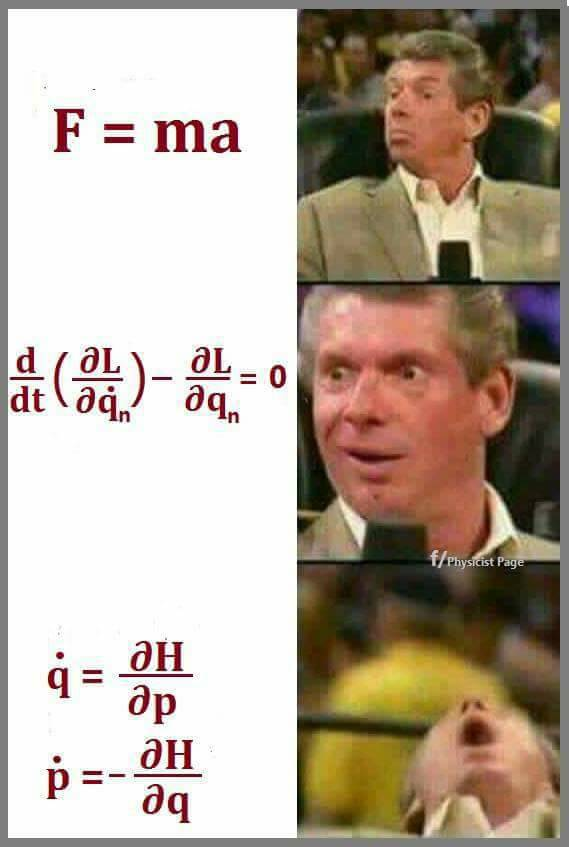
\includegraphics[width=5cm]{portada.jpg}
	%\label{fig.1}
%\end{figure}

\vspace*{4in}

\emph{\textquotedblleft ...El camino del progreso no es ni r\'apido ni f\'acil."}

\begin{flushright}
Marie Curie
\end{flushright}

\begin{large}

\end{large}
\end{center}

\end{titlepage}

\newpage
\thispagestyle{empty}
\ \\
\newpage
\setcounter{page}{1}


\pagestyle{plain}
\chapter*{Prefacio}

\textit{Este apunte ha sido escrito principalmente por I. Obreque a partir de las clases del Prof. Juan Crisostomo en el Departamento de Fisica de la Universidad de Concepción, y ha contado con las contribuciones de R. Stuardo, C. Riquelme y E. Arratia.} \\

\textit{El objetivo de estas notas es ser un apoyo para el curso de mecánica clásica I } 
\addcontentsline{toc}{chapter}{Prefacio}
\bigskip
\bigskip
\bigskip
\bigskip
\bigskip
\bigskip


\newpage



\thispagestyle{empty}
\tableofcontents
\listoffigures

\newpage
 
\setcounter{page}{1}

\chapter{Introducci\'on}\label{chapter1}

Antes de comenzar es útil recordar algunos conceptos previos, los cuales serán de utilidad en el desarrollo de estas notas. 

\section{Dinámica de una Partícula}
\subsection{Leyes de Newton}

La dinámica de las partículas puntuales esta determinada por las leyes de Newton

\begin{itemize}

\item{\textbf{Primera ley:}} Existen un conjunto de sistemas  llamados \textit{inerciales} donde toda partícula aislada, posee velocidad constante respecto a dichos sistemas. El reposo es naturalmente un caso particular de velocidad constante nula.

\item{\textbf{Segunda ley:}} Establece la forma de cuantificar la interacción de una partícula con el resto del universo, se enfatiza en que esta ley es solamente valida para partículas puntuales que por definición tienen masa constante.\\

\begin{equation}\label{1.1}
\vec{F}=m\vec{a} 
\end{equation}

en esta ley se cumple el principio de superposición, según el cual la fuerza neta o resultante sobre una partícula es la suma vectorial de cada fuerza aplicada como si cada una de ellas actuara sola. Esto significa que no hay efectos de interferencia entre las distintas fuerzas aplicadas sobre la particula.

\item{\textbf{Tercera ley:}} Cuando una partícula $A$ hace una fuerza $\vec{F}_{AB}$ sobre una partícula $B$ entonces la fuerza sobre $A$ debido a $B$ (denotada como $F_{BA}$) está relacionada con $\vec{F}_{AB}$ en la forma

\begin{equation}\label{1.2}
\vec{F}_{AB} = -\vec{F}_{BA}
\end{equation}

Es importante resaltar que esta ley lleva implícita la propagación instantánea de señales por lo cual su validez es muy limitada.

\end{itemize}

Por otra parte, esta leyes se pueden sustituir por sus equivalentes en términos del momento lineal 
$\vec{p}=m\vec{v}$. La primera ley nos dice que en los sistemas inerciales el momento lineal de una partícula aislada es contante, la segunda ley se escribe de la forma $\displaystyle\vec{F}=d\vec{p}/dt$ y la tercera ley es sustituida por el principio de conservación del momento para un sistema aislado de partículas.




\subsection{Teoremas de Conservación}

\textbf{\textit{Teorema 1:}} Si la fuerza neta es cero, entonces el momento $\displaystyle \vec{p}$ se conserva. \\

\textbf{Demostración}: \\

Si la suma de todas las fuerzas es cero, es decir, si

\begin{eqnarray} \nonumber
\sum_{i} \vec{F}_i &=& \vec{0} \\ \nonumber
\Rightarrow \frac{d\vec{p}}{dt}&=&0
\end{eqnarray} 

Por tanto

\begin{equation} \nonumber
\vec{p}=cte.
\end{equation}
\\


\textbf{\textit{Teorema 2:}} Si la suma de todos los torques es cero, entonces el momento angular se conserva. \\

\textbf{Demostración}: Considerando que $\displaystyle \sum_{i} \tau_i =\frac{d\vec{L}}{dt}$, si

\begin{eqnarray} \nonumber
\sum_{i} \vec{\tau}_i &=& 0 \\ \nonumber
\Rightarrow \frac{d\vec{L}}{dt} &=& 0
\end{eqnarray}

Por tanto

\begin{equation} \nonumber
L=cte.
\end{equation}







\subsection{Trabajo y Energía} 


\textbf{\textit{Definición:}} El trabajo es la capacidad que tiene una fuerza para mover un cuerpo. La magnitud física esta dada por

\begin{equation} \label{1.3}
W=\int_{A}^B \vec{F} \cdot \vec{dx}
\end{equation}

Para el caso donde la masa es constante y $F$ la fuerza neta se tiene

\begin{eqnarray} \nonumber
 W_{A \rightarrow B} &=& \int_{A}^B \vec{F} \cdot \vec{dx} = m \int_{A}^B \vec{a} \cdot \vec{dx} \\ \nonumber
 W_{A \rightarrow B} &=& \int_{t_A}^{t_B} \frac{d\vec{v}}{dt} \cdot \vec{v}dt =  \int_{t_A}^{t_B} \frac{d}{dt} \left(\underbrace{ \frac{1}{2} m \vec{v} \cdot \vec{v}}_{k}\right)dt \\ \label{1.4}
W_{A \rightarrow B} &=& \int_{t_A}^{t_B} \frac{dk}{dt}dt = k_A - k_B
\end{eqnarray}

Esta ultima igualdad es conocida como el teorema del trabajo y la energía.\\


En general, el trabajo depende de la trayectoria, sin embargo hay casos en los cuales es independiente de esta.





\subsection{Fuerzas Conservativas}
Una fuerza conservativa es aquella cuyo trabajo no depende de la trayectoria descrita por la partícula, sino unicamente de los las posiciones final e inicial presentes en el trayecto. Una consecuencia directa de este echo es que el trabajo de una fuerza conservativa  a lo largo de un camino cerrado es cero, es decir

\begin{equation} \label{1.5}
W=\oint \vec{F} \cdot \vec{dr}=0
\end{equation}

\textbf{\textit{Teorema:}} Si $\vec{F}$ es una fuerza conservativa entonces existe un campo escalar $U(\vec{r})$ tal que 

\begin{equation} \label{1.6}
\vec{F}=-\vec{\nabla}{U}
\end{equation}

\textbf{Demostración}: \\
\\ 

Si $\vec{F}$ es una fuerza conservativa, sabemos que 


\begin{equation} \nonumber
\oint_{C} \vec{F} \cdot \vec{dr}=0
\end{equation}


Usando el teorema de Stoke


\begin{eqnarray} \nonumber
\oint_{C} \vec{F} \cdot \vec{dr} &=& \oint_{S} \vec{\nabla} \times \vec{F} \cdot d\vec{s} \\ \nonumber
\Rightarrow \oint_{S} \vec{\nabla} \times \vec{F} \cdot d\vec{s} &=& 0
\end{eqnarray}

Por tanto

\begin{equation} \nonumber
\vec{\nabla} \times \vec{F} = 0
\end{equation}

finalmente

\begin{equation} \nonumber
\vec{F}=-\vec{\nabla}U
\end{equation}











\section{Notación de Einstein}

Se denomina notación de Einstein o convenio de suma de Einstein a la convención utilizada para abreviar la escritura de sumatorios, la cual consiste en suprimir el símbolo sumatorio en la presencia de indices de suma repetidos. \\
\\

\textbf{Ejemplo:} Una expresión de la forma 

\begin{equation} \nonumber
\sum_{i=3}^3 x_iy_i = x_1y_1 + x_2y_2+x_3y_3
\end{equation}

puede escribirse, usando notación de Einstein como

\begin{equation} \nonumber
x_iy_i
\end{equation}

\textbf{Nota}: Un indice de suma puede aparecer asociado a un termino en forma de producto hasta dos veces, por lo que expresiones como las siguientes \textbf{no} son validas

\begin{eqnarray} \nonumber
u_iv_iw_i\\ \nonumber
a_{mn}b_{m}c_{ml} 
\end{eqnarray}
















\chapter{Sistemas de Coordenadas y Cinematica}\label{chapter2}

Un objetivo de este curso es poder caracterizar el movimiento de una partícula en el espacio, esto es, poder describirla matemáticamente. Comenzaremos esta sección mostrando los sistemas que se utilizan con mas frecuencia para detallar de forma cuantitativa una posición en el espacio. Una vez estudiados nos ocuparemos de generalizar los conceptos asociados a un sistema de coordenadas cualquiera. Antes de comenzar es necesario definir algunos conceptos previos para nuestro estudio. \\
\\


\section{Sistemas de Referencia}

En física es necesario medir magnitudes las cuales están asociadas a sistema físico (posición, velocidad, etc), para esto es necesario tener presente un sistema de referencia, el cual esta conformado por los siguientes elementos: \\


\textbf{Observador:} 
Es aquel que es capaz de medir magnitudes asociadas a un sistema físico, con el objetivo de obtener información sobre el estado físico de dicho sistema \\
\\

\textbf{Sistema de Referencia:} Son físicamente reales y corresponden a un conjunto de instrumentos de medida diseñados para la determinación de cantidades físicas. \\
\\

\textbf{Punto de Referencia:} Punto o lugar desde el cual se efectuá una medición. \\
\\

\textbf{Sistema de Coordenadas:} Son construcciones puramente matemáticas que consisten en un conjunto en el cual por cada punto del espacio pasan tres \textit{curvas} linealmente independientes.  \\
\\


\textbf{\textit{Definición 1:}} Los valores medidos de las cantidades físicas son independientes de la elección del sistema coordenado. \\
\\

Existen muchos sistemas de coordenadas, por lo que la elección dependerá del tipo de movimiento que describa el cuerpo en estudio. A continuación estudiaremos los conceptos requeridos para un mejor estudio de los sistemas coordenados. \\

Nuestro espacio, como lo percibimos , posee tres dimensiones: Largo, ancho y alto. Como consecuencia podemos percibir tres direcciones de movimiento linealmente independientes. Geométricamente, una dirección es descrita por una curva en el espacio. \\
\\
 


\textbf{\textit{Definición 2:}} Una curva $\Gamma$ en el espacio es un conjunto $C\subseteq R^3$ que es la imagen de un intervalo $I\subset R$ bajo la aplicación :

\begin{eqnarray}\label{2.1}
\vec{r}:&I\longrightarrow  C \\         %mejorar aqui
\nonumber
& t \longrightarrow \vec{r}(t)
\end{eqnarray}


\begin{figure}[H]
	\centering
	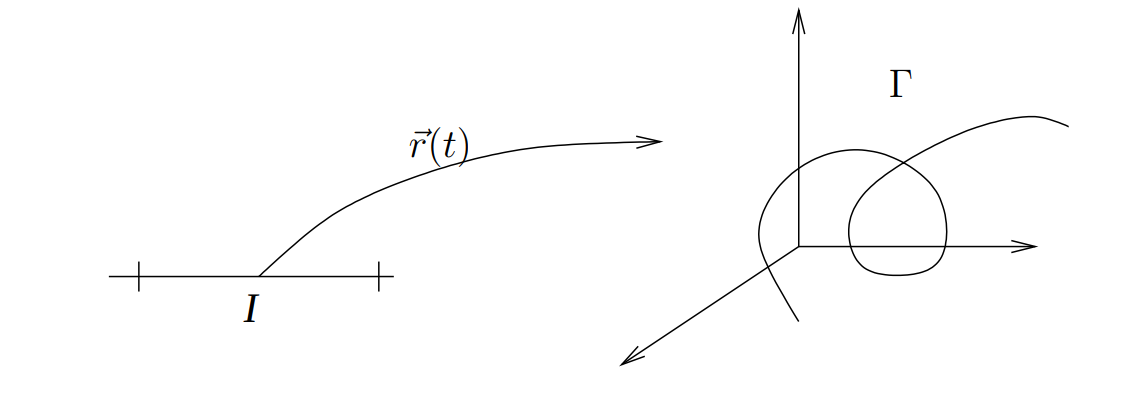
\includegraphics[width=14cm]{figura1.png}
	\caption{ Espacio del parametro de una curva y representacion de esta.}
	\label{fig.1}
\end{figure}

\textbf{Ejemplo}: Hélice \\

Una hélice es el nombre que recibe la curva cuyas tangentes forman un angulo constante con un plano, siguiendo una dirección fija en el espacio. Esta queda definida por la siguiente parametrización: 

\begin{eqnarray}\label{2.2}
\nonumber
x(\lambda)&=& rcos(w\lambda)\\
y(\lambda)&=& rsin(w\lambda)\\
\nonumber
z(\lambda)&=& b\lambda
\end{eqnarray}
\\
$r$: Radio \\	
$w$: Razon de giro angular \\
$b$: Avance en el sentido de $z$


\textbf{\textit{Definicion 3:}} Sea $\vec{x} = \vec{x}(\lambda)$ una curva, se define el vector tangente a la curva como:

\begin{equation} \label{2.3}
\Vec{T}(\lambda)= \frac{d \vec{x} }{ d\lambda }  %arreglar la flecha de la t
\end{equation}

\underline{Ejemplo}: Hélice
\\

Usando \eqref{2.2} se tiene 

\begin{equation}\label{2.4}
\displaystyle \vec{x}(\lambda)= rcos(w\lambda) \hat{\imath} +  rsin(w\lambda) \hat{\jmath} +b\lambda \hat{k}
\end{equation}

Luego el vector tangente es 

\begin{eqnarray} \nonumber
\vec{T}(\lambda) &=& \frac{d\vec{x}}{d\lambda} \\ \nonumber
&=& rw \left( -\sin (w\lambda)\hat{\imath} + \cos(w\lambda)\hat{\jmath} \right) + b\hat{k}.
\end{eqnarray} \\







\textbf{\textit{Proposicion 1}:} Sea $\vec{\xi}(x,y,z)$ un campo vectorial de $R^3$, luego siempre es posible encontrar una curva $\gamma \subset R^3$ tal que $\vec{\xi}$ sea tangente a cada punto de $\gamma$\\
\\
\textbf{Demostración}: 
\\

Sea $\gamma$ una curva  con parametrización $(\vec{x},I)$ cuyo vector tangente es paralelo a $\vec{\xi}$, entonces $\exists \ k \in R : $   

\begin{equation} \nonumber
\frac{d\vec{x}(\lambda)}{d\lambda}=k \vec{\xi}\left(x(\lambda),y(\lambda),z(\lambda)\right)
\end{equation}

Expresión que corresponde a tres ecuaciones diferenciales de primer orden no necesariamente lineales. Luego, por el teorema de existencia y unicidad estas tienen soluciones. \\

\textbf{Ejemplo}: Consideremos el caso en que $\vec{\xi}$ es constante , entonces 

\begin{eqnarray} \nonumber
\frac{d\vec{x}}{d\lambda} &=& k\vec{\xi} \\ \nonumber
d\vec{x} &=& k\vec{\xi} d\lambda \ \displaystyle / \int \\ 
\vec{x}(\lambda) &=& \lambda\vec{\xi} + \vec{x}_0 \label{2.5}
\end{eqnarray}

la cual corresponde a una linea recta.












\section{Coordenadas cartesianas}

Las coordenadas cartesianas corresponden a un conjunto de 3 ejes perpendiculares entre si, donde las coordenadas $(x,y,z)$ asociadas a un punto P son las distancias a los planos $YZ$,$XZ$ y $XY$, respectivamente. Para el sistema de coordenadas recién definido se puede escribir: 

\begin{equation} \label{2.6}
\vec{x}(x,y,z)= x\hat{\imath}+y\hat{\jmath}+z\hat{k} 
\end{equation}

Donde:  \\

\begin{eqnarray}{\nonumber}
-\infty&<x<&\infty \\
\nonumber
-\infty&<y<&\infty\\
\nonumber
-\infty&<z<&\infty
\end{eqnarray}



\begin{figure}[H]
	\centering
	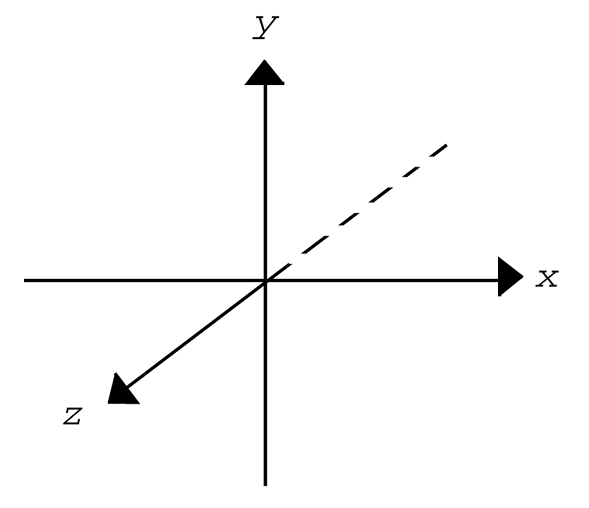
\includegraphics[width=8cm]{figura2.png}
	\caption{ Ejes cartesianos.}
	\label{fig.1}
\end{figure}

\begin{itemize}
\item x es la componente de $\vec{x}$ sobre el eje x 

\begin{equation}
\nonumber
x=\hat{\imath}\cdot \vec{x}
\end{equation}

\item y es la componente de $\vec{x}$ sobre el eje y

\begin{equation}{\nonumber}
y=\hat{\jmath}\cdot \vec{x}
\end{equation}

\item z es la componente de $\vec{x}$ sobre ele eje z

\begin{equation}{\nonumber}
z=\hat{k}\cdot \vec{x}
\end{equation}
\end{itemize}

La variación de los tres parámetros $xyz$ cubre todo el espacio, pero la variación de uno de ellos, mientras los otros quedan fijos, genera una curva llamada \textit{linea coordenada}

\subsection{Lineas coordenadas}


Puesto que hay tres parámetros libres, tendremos tres lineas coordenadas \\ 

\underline{\textbf{caso 1}}:

\begin{equation} \nonumber
x \in R \ \ \ ,\ \ \ y= y_0 \ \ \ ,  \ \ \ z=z_0
\end{equation}

Luego:

\begin{equation} \nonumber
\vec{x}(x,y_0,z_0)= x\hat{\imath} + y_0 \hat{\jmath} + z_0 \hat{k}
\end{equation}

En este caso tanto $y$ como $z$ estan fijos, pero, $x$ varia libremente generando una linea recta paralela al eje X  

\begin{figure}[H]
	\centering
	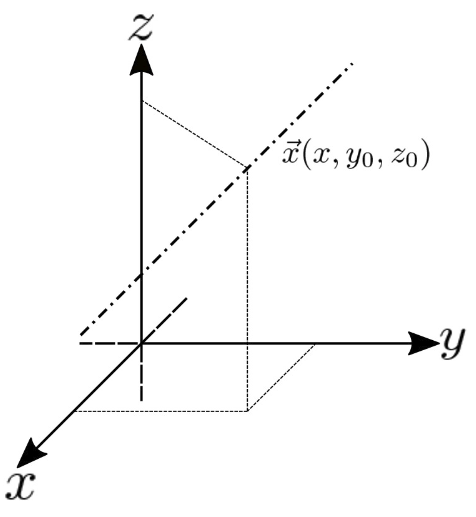
\includegraphics[width=7cm]{figura3.png}
	\caption{ Linea coordenada $y_0$,$z_0$ constante}
	\label{fig.1}
\end{figure}

 
\textbf{\underline{caso 2}:}

\begin{equation} \nonumber
x = x_0 \ \ \ ,\ \ \ y= y_0 \ \ \ ,  \ \ \ z \in R
\end{equation}
 
 Luego:
 
 \begin{equation} \nonumber
 \vec{x}(x_0,y_0,z)= x_0\hat{\imath} + y_0 \hat{\jmath} + z \hat{k}
 \end{equation}

En este caso la linea coordenada es una recta paralela al eje Z. \\


\begin{figure}
	\centering
	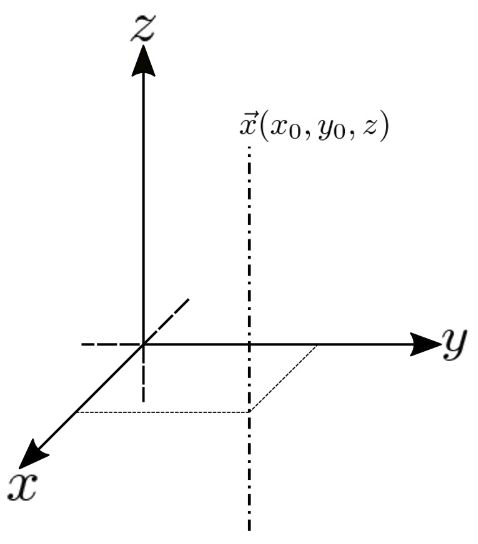
\includegraphics[width=7cm]{figura4.png}
	\caption{ Linea coordenada $x_0$,$y_0$ constante.}
	\label{fig.1}
\end{figure}

\textbf{\underline{caso 3}:} 

\begin{equation} \nonumber
x = x_0 \ \ \ ,\ \ \ y \in R \ \ \ ,  \ \ \ z=z_0
\end{equation}

Luego:

\begin{equation} \nonumber
\vec{x}(x_0,y,z_0)= x_0\hat{\imath} + y \hat{\jmath} + z_0 \hat{k}
\end{equation}

La linea coordenada corresponde a una recta paralela al eje Y. \\


\begin{figure}
	\centering
	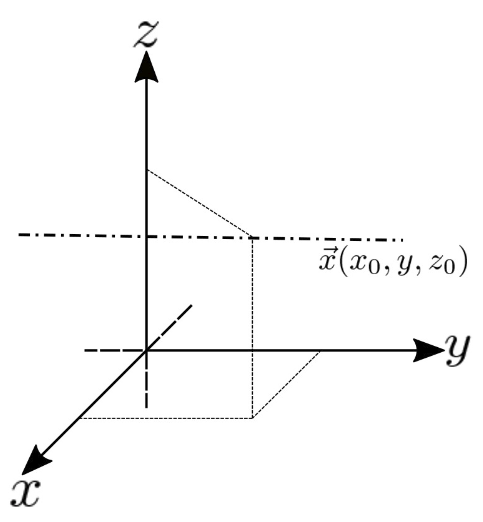
\includegraphics[width=7cm]{figura5.png}
	\caption{ Linea coordenada $x_0$,$z_0$ constante.}
	\label{fig.1}
\end{figure}


 Por tanto, en cada punto de $R^3$ pasan tres curvas rectas que se interceptan perpendicularmente. Se puede concluir que este sistema de coordenadas permite describir direcciones rectas. 
 
 
 
 
 
  
 
 
 
 \subsection{Cosenos directores}
Un vector $\vec{A}$ en coordenadas cartesianas se puede descomponer como

\begin{equation}
\vec{A}=A_x \hat{\imath} + A_y \hat{\jmath} + A_z \hat{k}
\end{equation}

donde $A_x$, $A_y$ y $A_z$ son las componentes del vector $\vec{A}$  a los largo del eje $X$, $Y$ y $Z$.

\begin{eqnarray} \nonumber
A_x &=& \hat{\imath} \cdot \vec{A} = \norm{\vec{A}} \cos \alpha \\ \nonumber
A_y &=& \hat{\jmath} \cdot \vec{A} = \norm{\vec{A}} \cos \beta \\  \nonumber
A_z &=& \hat{k} \cdot \vec{A} = \norm{\vec{A}} \cos \gamma 
\end{eqnarray}

donde: \\
\\
$\alpha$: angulo que forma $\vec{A}$ con el eje X.\\
$\beta$: angulo que forma $\vec{A}$ con el eje Y. \\
$\gamma$: angulo que forma $\vec{A}$ con el eje Z.
 \\

 \textbf{\underline{Nota}:} $\cos \alpha$, $\cos \beta$ y $\cos \gamma$ son los cosenos directores del vector $\vec{A}$. \\
 

Luego , podemos escribir el vector $\vec{A}$ en función de los cosenos directores

\begin{eqnarray} \nonumber
\vec{A}&=&A_x \hat{\imath} + A_y \hat{\jmath} + A_z \hat{k} \\ \nonumber
&=& \norm{\vec{A}} \cos\alpha \ \hat{\imath} + \norm{\vec{A}} \cos \beta \ \hat{\jmath} + \norm{\vec{A}} \cos \gamma \ \hat{k} \\ 
&=& \norm{\vec{A}} \left( \cos\alpha \ \hat{\imath} + \cos \beta \ \hat{\jmath} + \cos \gamma \ \hat{k} \right) \label{2.8}
\end{eqnarray}

\textbf{\textit{Proposición 2:}} Los cosenos directores satisfacen la expresión

\begin{equation}\label{2.9}
\cos^2 \alpha + \cos^2 \beta + \cos^2 \gamma = 1
\end{equation}

\textbf{Demostración}: \\

Usando \eqref{2.8} calculemos la norma del vector $\vec{A}$ 

\begin{eqnarray} \nonumber
\norm{\vec{A}} &=&\sqrt{\norm{\vec{A}}^2 \left( \cos^2 \alpha + \cos^2 \beta + \cos^2 \gamma \right)} \\ \nonumber
&=& \norm{\vec{A}} \sqrt{\cos^2 \alpha + \cos^2 \beta + \cos^2 \gamma}
\end{eqnarray} 

Por tanto

\begin{equation}
\cos^2 \alpha + \cos^2 \beta + \cos^2 \gamma = 1.
\end{equation}














\section{Coordenadas Esfericas}

Las coordenadas esféricas $(r,\phi,\theta)$ se definen como

\begin{eqnarray} \nonumber
x(r,\phi,\theta) &=& r \cos \phi \sin \theta \\ \label{2.11}
y(r,\phi,\theta) &=& r \sin \phi \sin \theta \\ \nonumber
x(r,\phi,\theta) &=& r \cos \theta
\end{eqnarray}

 
 donde: \\
 \\
\begin{eqnarray} \nonumber
r &\in& [0, \infty) \\ \nonumber
\phi &\in& [o,2\pi) \\ \nonumber
\theta &\in& [0, \pi]
\end{eqnarray}
 


La posición del punto P en coordenadas esféricas es

\begin{equation}\label{2.12}
 \vec{x}(r,\phi,\theta)=r \cos \phi \sin \theta \ \hat{\imath} +  r \sin \phi \sin \theta \ \hat{\jmath} + r \cos \theta \hat{k} 
\end{equation}

Notemos que $r$ es la magnitud de $\norm{\vec{x}}$. En efecto

\begin{eqnarray} \nonumber
\norm{\vec{x}}&=&=\sqrt{r^2 \cos^2 \phi \sin^2 \theta +  r^2 \sin^2 \phi \sin^2 \theta + r^2 \cos^2 \theta } \\ \nonumber
&=&  r \sqrt{\left(\cos^2 \phi +  \sin^2 \phi \right) \sin^2 \theta  + \cos^2 \theta} \\ \nonumber
&=& r \sqrt{\sin^2 \theta + \cos^2 \theta} \\ \nonumber
&=& r
\end{eqnarray}

Considerando este ultimo resultado se tiene que $\displaystyle \frac{\vec{x}}{r}$ es un vector unitario, por lo que definimos

\begin{equation}\label{2.13}
\hat{r}(\phi,\theta)=\cos{\phi}\sin{\theta} \ \hat{\imath} + \sin{\phi}\sin{\theta} \ \hat{\jmath} + \cos{\theta} \hat{k}
\end{equation}

Luego:

\begin{equation}\label{2.14}
\vec{x}(r,\phi,\theta)=r\hat{r}(\phi,\theta)
\end{equation}









\subsection{Lineas coordenadas}

Puesto que hay tres parámetros libres que varían de forma independiente, tendremos tres lineas coordenadas\\

\textbf{\underline{Caso 1}:}

\begin{equation}\nonumber
r \geq 0 \ \ \ , \ \ \ \phi=\phi_0 \ \ \ , \ \ \ \theta=\theta_0 
\end{equation}

Luego:

\begin{equation}
\vec{x}(r,\phi_0,\theta_0)=r\hat{r}(\phi_0,\theta_0)
\end{equation}
\\
La linea coordenada corresponde a una recta que pasa por el origen  con vector direccional 

\begin{equation}
\vec{\xi}(\phi_0,\theta_0)= \hat{r}(\phi_0,\theta_0) %IMAGEN AQUIII!!!!!!!
\end{equation}


\begin{figure}[H]
	\centering
	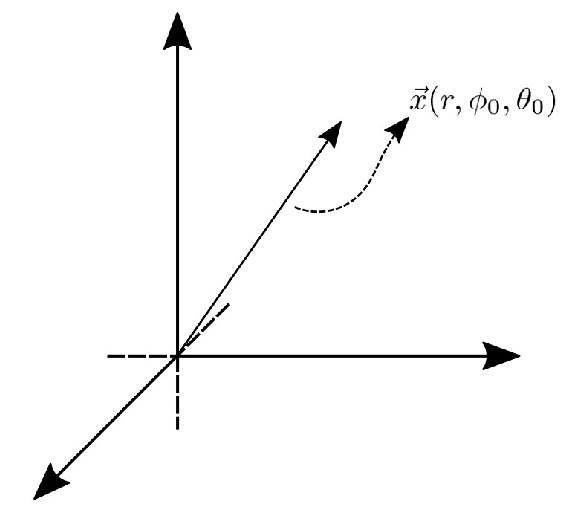
\includegraphics[width=7cm]{figura321.png}
	\caption{ Linea coordenada $\theta_0$,$\phi_0$ constante.}
	\label{fig.1}
\end{figure}

\textbf{\underline{Caso 2}:}

\begin{equation} \nonumber
r=r_0 \ \ \ , \ \ \  0 \leq \phi < 2\pi \ \ \ , \ \ \ \theta= \theta_0 
\end{equation}

Luego

\begin{eqnarray} \nonumber
x(r_0,\phi,\theta_0)&=& r_0 \cos{\phi}\sin{\theta_0} \\ \label{2.17}
y(r_0,\phi,\theta_0)&=& r_0 \sin{\phi}\sin{\theta_0}  \\ \nonumber
z(r_0,\phi,\theta_0)&=& r_0 \cos{\theta_0}= z_0
\end{eqnarray}

podemos escribir lo anterior como

\begin{eqnarray}
x^2 + y^2 = r_{0}^2 \sin^2{\theta_0} \\ \nonumber
z_{0} = r_0 \cos{\theta_0} 
\end{eqnarray}

Lo cual corresponde a una circunferencia de radio $r_0 \sin{\theta_0}$ y  centro en $r_0 \cos{\theta_0} \hat{k}$. 


\begin{figure}[H]
	\centering
	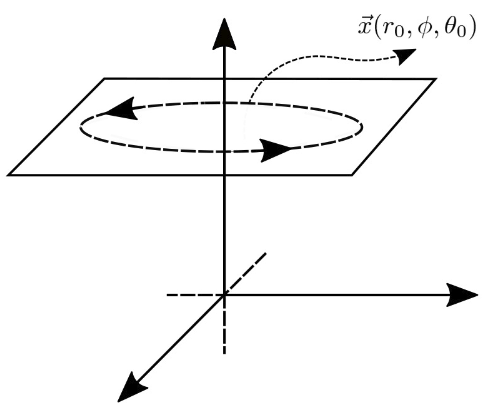
\includegraphics[width=7cm]{figura52.png}
	\caption{ Linea coordenada $r_0$,$\theta_0$ constante.}
	\label{fig.1}
\end{figure}

\textbf{\underline{Caso 3}:}

\begin{equation} \nonumber
r=r_0 \ \ \ , \ \ \  \phi=\phi_0 \ \ \ , \ \ \ 0 \leq \theta \leq \pi 
\end{equation}

Luego:

\begin{eqnarray} \nonumber
x(r_0,\phi_0,\theta) &=& r_0 \cos{\phi_0}\sin{\theta} \\ \label{2.19}
y(r_0,\phi_0,\theta) &=& r_0 \sin{\phi_0}\sin{\theta} \\ \nonumber
z(r_0,\phi_0,\theta) &=& r_0 \cos{\theta}
\end{eqnarray}

Notemos que podemos reescribir lo anterior eliminando el parametro $\theta$

\begin{eqnarray} \label{2.20}
x^2 + y^2 + z^2 &=& r_0^2 \\
y &=&\tan{\phi_0} \ x \label{2.21}
\end{eqnarray}

Ecuaciones correspondientes a una esfera de radio $r_0$ y un plano que contiene al eje Z. Por tanto la linea coordenada para este caso es la interseccion entre el plano y la esfera, lo que corresponde a una circunferencia de radio $r_0$ que corta en $z=\pm r_0$.
 
 \begin{figure}
	\centering
	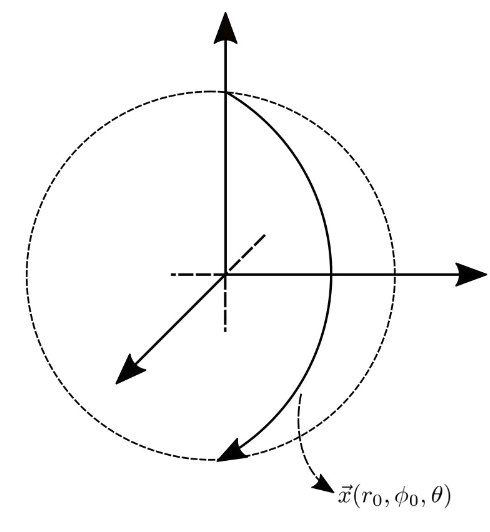
\includegraphics[width=7cm]{figura51.png}
	\caption{ Linea coordenada $r_0$,$\phi_0$ constante.}
	\label{fig.1}
\end{figure}
 





\section{Vectores Direccionales}


Una vez escogido el sistema coordenado, en términos mas generales, un punto P arbitrario del espacio queda determinado por el llamado vector posición $\displaystyle\vec{x}(x^1,x^2,x^3)$ el cual depende de tres parámetros libres que definen el sistema coordenado, denotado por $Ox^1x^2x^3$.

Donde:

\begin{itemize}
\item $x^1$: Genera la curva coordenada $\vec{x}(x^1,x_0^2,x_0^3)$, con $x_0^2$ y $x_0^3$ valores fijos de referencia.
\item $x^2$: Genera la curva coordenada $\vec{x}(x_0^1,x^2,x_0^3)$, con $x_0^1$ y $x_0^3$ valores fijos de referencia. 
\item $x^3$: Genera la curva coordenada $\vec{x}(x_0^1,x_0^2,x^3)$, con $x_0^1$ y $x_0^2$ valores fijos de referencia. 
\end{itemize}


\textbf{Ejemplo 1}: Coordenadas cartesianas 

\begin{equation}\nonumber
x^1=x \ \ \ , \ \ \ x^2 = y \ \ \ ,  \ \ \ x^3=z
\end{equation}

\textbf{Ejemplo 2}: Coordenadas esfericas

\begin{equation}\nonumber 
x^1=r \ \ \ , \ \ \ x^2 = \phi \ \ \ ,  \ \ \ x^3=\theta
\end{equation} 
\\

Antes de continuar consideremos una notación mas compacta

\begin{equation}
\vec{x}(x^1,x^2,x^3):=\vec{x}(x^a) \ \ \ , \ \ \ a=1,2,3
\end{equation}


Puesto que cada parámetro puede variar libremente generando una curva coordenada, estas tendrán también asociadas vectores tangentes los cuales llamaremos \textit{vectores direccionales} de la linea coordenada.

En cada punto $P$ $\in R^3$ , con vector posición $\vec{x}(x^a)$ en el  sistema de coordenada $Ox^1x^2x^3$, pasan tres vectores direccionales, los cuales están dados por

\begin{eqnarray} \label{2.23}
\vec{e}_1 &=& \frac{\partial \vec{x}}{\partial x^1} \\
\vec{e}_2 &=& \frac{\partial \vec{x}}{\partial x^2} \\ \label{2.24}
\vec{e}_3 &=& \frac{\partial \vec{x}}{\partial x^3}    \label{2.25}
\end{eqnarray}

\begin{figure}[H]
	\centering
	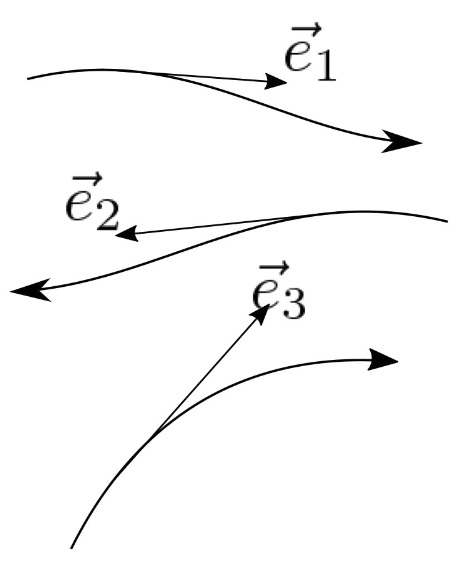
\includegraphics[width=7cm]{figura61.png}
	\caption{ vectores direccionales.}
	\label{fig.1}
\end{figure}

\textbf{\underline{Notación}:}

\begin{equation} \nonumber
\vec{e}_a= \frac{\partial \vec{x}}{\partial x^a} \ \ \ , \ \ \  a=1,2,3 
\end{equation}
\\

\textbf{\textit{Definición 4:}} El vector direccional a la linea coordenada 	generada por $x^a$,$ \ a=1,2,3$, es dado por 


\begin{equation} \label{2.26}
\vec{e}_a= \frac{\partial \vec{x}}{\partial x^a} \ \ \ , \ \ \  a=1,2,3 
\end{equation}
\\


\textbf{\underline{Nota}:} Los vectores direccionales no son necesariamente ortogonales entre si, es decir, el producto interno entre dos de ellos no es necesariamente nulo.\\ \\

\textbf{\textit{Definición 5:}} Los vectores unitarios $\displaystyle\hat{e}_a$ , con $a=1,2,3$, se obtienen a partir de los vectores direccionales en la forma

\begin{equation} \label{2.27}
\hat{e}_a =  \frac{\vec{e}_a}{\norm{\vec{e}_a}} \ \ \ , \ \ \ a=1,2,3
\end{equation}

donde

\begin{equation} \label{2.28}
\norm{\vec{e}_a}= \sqrt{\vec{e}_a \cdot \vec{e}_a}.
\end{equation}

Los vectores direccionales pueden variar de un punto a otro en el espacio, por lo que estos también dependen de las coordenadas, es decir

\begin{equation}  \nonumber
\vec{e}_a(x^1,x^2,x^3):= \vec{e}_a(x^b)
\end{equation}

En general, de la misma forma ocurrirá con los vectores unitarios


\begin{equation} \nonumber
\hat{e}_a(x^1,x^2,x^3):= \hat{e}_a(x^b).
\end{equation}

\textbf{\textit{Proposición 3:}} Los vectores unitarios $\displaystyle\hat{e}_a$ no se anulan en ningun punto de $R^3$. \\ \\


\textbf{Ejemplo 1}: Coordenadas cartesianas

\begin{equation} \nonumber
\vec{x}(x,y,z)= x \hat{\imath} + y \hat{\jmath} + z \hat{k}
\end{equation}

\begin{eqnarray} \label{2.29}
\vec{e}_1&=&\frac{\partial \vec{x}}{\partial x} = \hat{\imath} \\
\vec{e}_2&=&\frac{\partial \vec{x}}{\partial y} = \hat{\jmath} \\ \label{2.30}
\vec{e}_3&=&\frac{\partial \vec{x}}{\partial z} = \hat{k} \label{2.31}
\end{eqnarray}

\textbf{Ejemplo 2}: Coordenadas esféricas


\begin{equation} \nonumber
 \vec{x}(r,\phi,\theta)=r \cos \phi \sin \theta \ \hat{\imath} +  r \sin \phi \sin \theta \ \hat{\jmath} + r \cos \theta \hat{k} 
\end{equation}

\begin{eqnarray}  \label{2.32}
\vec{e}_1&=&\frac{\partial \vec{x}}{\partial r} = \cos{\phi}\sin{\theta}  \ \hat{\imath} + \sin{\phi}\sin{\theta} \ \hat{\jmath} + \cos{\theta} \ \hat{k} \\
\vec{e}_2&=&\frac{\partial \vec{x}}{\partial \phi} = r\sin{\theta}\left(-\sin{\phi} \ \hat{\imath} + \cos{\phi} \ \hat{\jmath} \right)  \\ \label{2.33}
\vec{e}_3&=&\frac{\partial \vec{x}}{\partial \theta} = r\cos{\phi}\cos{\theta} \ \hat{\imath} + r\sin{\phi}\cos{\theta}  \ \hat{\jmath} \ -r \sin{\theta} \ \hat{k}  \label{2.34}
\end{eqnarray}


\begin{figure}[H]
	\centering
	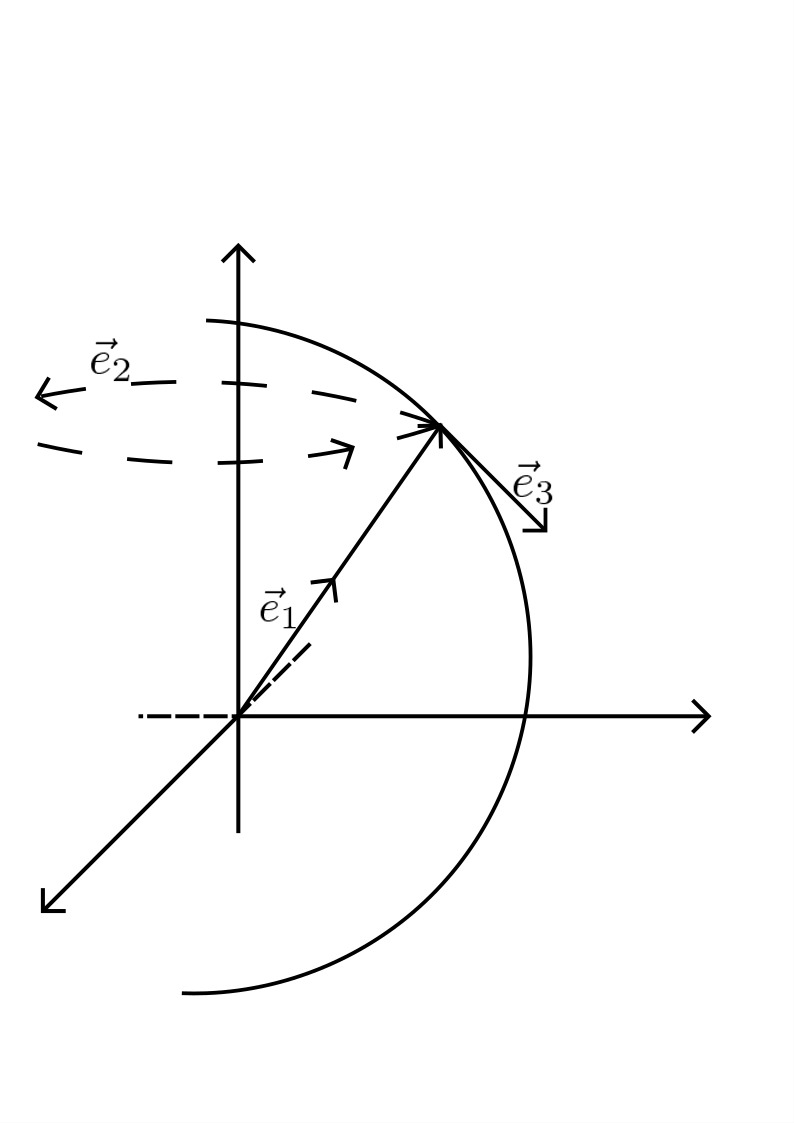
\includegraphics[width=7cm]{figura7.jpeg}
	\caption{ Vectores direccionales en coordenadas esféricas.}
	\label{fig.1}
\end{figure}

Los vectores unitarios estan dados por

\begin{eqnarray}
\hat{r} &=& \cos{\phi}\sin{\theta}  \ \hat{\imath} + \sin{\phi}\sin{\theta} \ \hat{\jmath} + \cos{\theta} \ \hat{k} \\
\hat{\phi} &=& - \sin{\phi} \ \hat{\imath}+ \cos{\phi} \ \hat{\jmath} \\
\hat{\theta} &=& \cos{\phi}\cos{\theta} \ \hat{\imath} + \sin{\phi}\cos{\theta}  \ \hat{\jmath} \ -\sin{\theta} \ \hat{k} 
\end{eqnarray}

Luego, mediante \eqref{2.27} podemos obtener los vectores direccionales en función de los vectores unitarios $\hat{r}, \hat{\phi}$ y $\hat{\theta}$

\begin{eqnarray}
\vec{e}_1 &=& \hat{r} \\
\vec{e}_2 &=& r\sin{\theta} \hat{\phi} \\
\vec{e}_3 &=& r \hat{\theta} .  % agregar algo mas de mis apuntes !!!
\end{eqnarray}

\textbf{\underline{Observación}:} Los vectores $\hat{e}_a$ y $\vec{e}_a$ no contienen la misma información geometrica, puesto que $\vec{e}_a$ podria indeterminarse en algun punto. Los vectores unitarios $\hat{e}_a$ no se anulan ni se indeterminan.
 \\
 \\

\textbf{\textit{Definición 6:}} Un sistema de coordenadas posee asociado a el un conjunto de vectores direccionales $\{ e_{a} \}_{a=1}^3$, los cuales de ahora en adelante asignaremos como una base para $R^3$, por lo tanto un campo vectorial $ \vec{A} \in R^3 $ se puede escribir en terminos de esta base.


\begin{eqnarray}
\vec{A} &=& A^1 \vec{e}_1 + A^2 \vec{e}_2 + A^2 \vec{e}_2 \\ \label{2.42}
&=& \sum_{a=1}^3 A^a \vec{e}_a
\end{eqnarray} 

donde $A^a$ es la componente del vector $\vec{A}$ a lo largo del eje $x^a$.\\


\textbf{\underline{observación}:} Recordemos que $\vec{A}$ es un campo vectorial, esto significa que depende de las coordenadas $x^a$ con $a=1,2,3$ , al igual que los vectores direccionales, por tanto

\begin{equation} \nonumber
 \vec{A}(x^b) = \sum_{a=1}^3 A^a(x^c) \vec{e}_a (x^d).
\end{equation}








\section{Metrica y Elemento de Linea}

Sea $\gamma $ una curva en el espacio, la longitud de un elemento $ds$ en coordenadas cartesianas esta dada por

\begin{equation}
ds^2=dx^2 +  dy^2 + dz^2
\end{equation}

considerando que $\vec{dx}=dx\hat{\imath}+dy\hat{\jmath}+ dz\hat{k}$ se tiene que 

\begin{equation} \label{2.44}
ds^2 = \vec{dx} \cdot \vec{dx} 
\end{equation}

 En general, la expresión \eqref{2.44} se denomina elemento de linea y es independiente del sistema de coordenadas que se utilice. Este corresponde a la distancia entre dos puntos infinitesimalmente  cercanos, los cuales están unidos mediante un segmento $ds$ que es aproximado a una linea recta. \\

En un sistema de coordenadas  $ O  x^1 x^2 x^3$ se tiene que 


\begin{eqnarray}
d\vec{x}&=& d\vec{x}(x^a) \nonumber \\
&=&d\vec{x}(x^1,x^2,x^3) \nonumber \\
&=&\frac{\partial\vec{x}}{\partial x^1}dx^1+\frac{\partial \vec{x}}{\partial x^2}dx^2 + \frac{\partial \vec{x}}{\partial x^3}dx^3 \nonumber \\
&=& \displaystyle\sum_{a=1}^3 \frac{\partial \vec{x}}{\partial x^a}dx^a \nonumber \\ \label{2.45}
&=& \displaystyle\sum_{a=1}^3 \vec{e}_a dx^a 
\end{eqnarray}

Reemplazando \eqref{2.45} en \eqref{2.44} se tiene que 

\begin{eqnarray}
ds^2&=& d\vec{x} \cdot d\vec{x} \nonumber \\
&=& \displaystyle\sum_{a=1}^3 \vec{e}_a dx^a \cdot \displaystyle\sum_{b=1}^3 \vec{e}_b dx^b \nonumber \\  \label{2.46}
&=& \displaystyle\sum_{a=1}^3\displaystyle\sum_{b=1}^3\vec{e}_a\vec{e}_b dx^a dx^b
\end{eqnarray}



\textbf{\textit{Definición}:} Se define la métrica $g_{ab}(x^c)=g_{ab}(x^1,x^2,x^3)$ como:

\begin{equation}
\nonumber
g_{ab}=\vec{e}_a(x^d) \cdot \vec{e}_b(x^e)
\end{equation}

Con esta definición podemos reescribir \eqref{2.46} como: 

\begin{equation} \label{2.47}
ds^2 = \displaystyle\sum_{a=1}^3\sum_{b=1}^3 g_{ab}dx^adx^b
\end{equation}

Desarrollando esta suma obtenemos :

\begin{eqnarray*}
\nonumber
ds^2 &=& \displaystyle\sum_{b=1}^3 g_{1b}dx^1dx^b + g_{2b}dx^2 dx^b + g_{3b}dx^3 dx^b \\
&=& \lefteqn{ g_{11}(dx^1)^2 + g_{12} dx^1 dx^2 + g_{13} dx^1 dx^3  + g_{21} dx^2 dx^1+} \\ 
 &&  g_{22}(dx^2)^2 + g_{23}dx^2 dx^3 + g_{31} dx^3 dx^1 + g_{32} dx^3 dx^2 + \\
 &&  g_{33} (dx^3)^2
\end{eqnarray*}


Notemos que la métrica $g_{ab}$ es simétrica bajo el intercambio de indices $"a"$ y $"b"$ ($g_{ab}=g_{ba}$). Para visualizar de forma mas clara esta propiedad escribamos la métrica como una matriz de $  3 \times 3$\\
\\

\begin{eqnarray} 
g_{ab}&=&
\left(
\begin{array}{ccc}
g_{11} & g_{12} & g_{13} \\ \label{2.48}
g_{21} & g_{22} & g_{23} \\
g_{31} & g_{32} & g_{33}
\end{array}
\right) \\ \nonumber
\\ 
&=& 
\left(
\begin{array}{ccc} \
\vec{e}_{1} \cdot \vec{e}_1 & \vec{e}_1 \cdot \vec{e}_2 & \vec{e}_1 \cdot \vec{e}_3 \\ \nonumber
\vec{e}_2 \cdot \vec{e}_1 & \vec{e}_2 \cdot \vec{e}_2 & \vec{e}_2 \cdot \vec{e}_3 \\ \nonumber
\vec{e}_3 \cdot \vec{e}_1 & \vec{e}_3 \cdot \vec{e}_2 & \vec{e}_3 \cdot \vec{e}_3 \nonumber
\end{array}
\right) \\ \nonumber
\\ 
&=&
\left(
\begin{array}{ccc}
\vec{e}_1 \cdot \vec{e}_1 & \vec{e}_2 \cdot \vec{e}_1 & \vec{e}_3 \cdot \vec{e}_1 \\ \nonumber
\vec{e}_1 \cdot \vec{e}_2 & \vec{e}_2 \cdot \vec{e}_2 & \vec{e}_3 \cdot \vec{e}_2 \\
\vec{e}_1 \cdot \vec{e}_3 & \vec{e}_2 \cdot \vec{e}_3 & \vec{e}_3 \cdot \vec{e}_3
\end{array}
\right)
\\
&=& g_{ba} \nonumber
\end{eqnarray}    
\\

Por tanto, en lenguaje matricial  $g=g^t$.
\\





\textbf{Ejemplo 1}: Coordenadas cartesianas \\


En coordenadas cartesianas los vectores direccionales son : \\

 \begin{equation}
 \nonumber 
 \vec{e}_1 = \hat{\imath}  \ \ \ \ \ \ \  \vec{e}_2 = \hat{\jmath}  \ \ \ \ \ \ \ \vec{e}_3 = \hat{k}
 \end{equation}

Por otra parte los únicos elementos de la métrica distintos de cero son los que tienen subíndices iguales.

\begin{equation}
\nonumber
g_{11}=1 \ \ \ \ \ \ \ g_{22}=1 \ \ \ \ \ \ \ g_{33}=1
\end{equation}

En forma matricial:


\[ g_{ab} =
\left( \begin{array}{cccc} 
 1 & 0 & 0  \\ 
 0 & 1 & 0  \\
 0 & 0 & 1  
\end{array} \right) \]

Por tanto el elemento de linea esta dado por :

\begin{equation}
ds^2= dx^2 + dx^2 + dz^2
\end{equation}

\textbf{\underline{Observación:}} En este caso $g_{ab}$ es conocida como métrica de Euclides
\\
\\

\textbf{Ejemplo 2:} Coordenadas esféricas \\


En coordenadas esféricas los elementos de la métrica distintos de cero son los que tienen subíndices iguales.

\begin{eqnarray} 
g_{11}&=& \vec{e}_1 \cdot \vec{e}_1 = 1 \nonumber \\
g_{22}&=& \vec{e}_2 \cdot \vec{e}_2 = r^2 \sin ^2\theta \nonumber \\
g_{33}&=& \vec{e}_3 \cdot \vec{e}_3 = r^2 \nonumber
\end{eqnarray}
\\
En forma matricial:

\begin{eqnarray} \nonumber
g_{ab} &=&
\left(
 \begin{array}{ccc} 
 \vec{e}_1 \cdot \vec{e}_1 & \vec{e}_1 \cdot \vec{e}_2 & \vec{e}_1 \cdot \vec{e}_3  \\ 
 \vec{e}_2 \cdot \vec{e}_1 & \vec{e}_2 \cdot \vec{e}_2 & \vec{e}_2 \cdot \vec{e}_3  \\
 \vec{e}_3 \cdot \vec{e}_1 & \vec{e}_3 \cdot \vec{e}_3 & \vec{e}_3 \cdot \vec{e}_3  \\
\end{array} 
\right) \\ \nonumber
\\ \nonumber
&=&  \displaystyle \left( \begin{array}{ccc}
\hat{r} \cdot \hat{r} & 0 &  0 \\
0 & r^2 sin^2\theta \hat{\phi} \cdot \hat{\phi} &  0 \\
0 & 0 &  r^2 \hat{\theta} \cdot \hat{\theta} \\
\end{array}
\right) \\ \nonumber
\\ 
&=& \displaystyle \left( \begin{array}{ccc} \label{2.50}
1 & 0 &  0 \\
0 & r^2 sin^2\theta &  0 \\
0 & 0 &  r^2  \\
\end{array}
\right) 
\end{eqnarray}
 

Por tanto, el elemento de linea en coordenadas esfericas esta dado por

\begin{eqnarray}
ds^2&=& \sum_{a=1}^3 \sum_{b=1}^3 g_{ab}dx^adx^b \nonumber \\
&=& \sum_{b=1}^3 g_{1b} drdx^b + \sum_{b=1}^3 g_{2b} d\phi dx^b + \sum_{b=1}^3 g_{3b}d\theta dx^b \nonumber \\
&=& \lefteqn{g_{11}(dr)^2 + g_{12}drd\phi + g_{13}drd\theta +} \nonumber \\
&& g_{21}drd\phi + g_{22}(d\phi)^2 + g_{23}d\phi d\theta + \nonumber \\
&& g_{31}d\theta dr + g_{32}d\theta d\phi + g_{33}(d\theta)^2 \nonumber \\ \label{2.51}
&=& dr^2 + r^2 \sin ^2 \theta d\phi^2 + r^2d\theta^2
\end{eqnarray}
\\
\\

\textbf{\underline{Observación}:} Escribamos los diferenciales como una matriz columna de orden   $ 3 \times 1 $:


\[ dx^a \longrightarrow dX=
\left( \begin{array}{c}
 dx^1  \\ 
 dx^2  \\
 dx^3
\end{array} \right) \]


Así, el elemento de linea se puede representar matricialmente como:


\begin{equation} \label{2.52}
dS^2=dX^tgdX
\end{equation}

 Luego , podemos obtener \eqref{2.51} mediante \eqref{2.52} 
 
\begin{eqnarray}
\nonumber
ds^2 &=& 
\left(
\begin{array}{ccc}
dr & d\phi & d\theta
\end{array}
\right)
\left(
\begin{array}{ccc}
1 & 0 & 0 \\
0  & r^2 \sin\theta & 0 \\
0 & 0 & r^2
\end{array}
\right)
\left(
\begin{array}{c}
dr \\
d\phi \\
d\theta
\end{array}
\right) \\
&=& \left(
\begin{array}{ccc} \nonumber
dr & d\phi & d\theta
\end{array}
\right) 
\left(
\begin{array}{c}
dr \\
r^2\sin^2\theta d\phi \\
r^2 d\theta
\end{array}
\right) \\ \nonumber
\\ \nonumber
&=& dr^2 + r^2 \sin ^2 \theta d\phi^2 + r^2d\theta^2 \nonumber
\end{eqnarray}
\\


\textbf{\underline{Observación 2}:} Notemos que el modulo de los vectores direccionales se pueden escribir como  :

\begin{eqnarray}
\norm{\vec{e_1}}&=&\sqrt{\vec{e_1} \cdot \vec{e_1} }= g_{11} \nonumber \\
\norm{\vec{e_2}}&=&\sqrt{\vec{e_2} \cdot \vec{e_2} }= g_{22} \nonumber \\
\norm{\vec{e_3}}&=&\sqrt{\vec{e_3} \cdot \vec{e_3} }= g_{33} \nonumber 
\end{eqnarray}

Es decir:

\begin{equation}
\norm{\vec{e_a}}= \sqrt{g_{aa}} \ , \ a = 1,2,3.
\end{equation}

Luego los vectores unitarios se pueden escribir como 

\begin{equation} \label{2.54}
\uvec{e}_a = \frac{\vec{e}_a}{\sqrt{g_{aa}}} \ , \ a=1,2,3.
\end{equation}



\textbf{\textit{Definición:}} Se define la delta de Kronecker como

\begin{eqnarray} \label{2.55}
 \delta_{i,j} =
\left\{ \begin{array}{ccc} 
 1 & {\rm  si~~} i=j   \\ 
 0 & {\rm  si~~} i\ne j  \\  
\end{array} \right.
\end{eqnarray}

Escribiendo \eqref{2.55} en forma matricial 

\begin{eqnarray} \nonumber
 \delta_{ab} &=&
\left( \begin{array}{cccc} 
 \delta_{11} & \delta_{12} & \delta_{13}  \\ 
 \delta_{21} & \delta_{22} & \delta_{23} \\
 \delta_{31} & \delta_{32} & \delta_{33}  
\end{array} \right) \\ \nonumber
\\  
&=& \left( \begin{array}{cccc}  \label{2.56}
 1 & 0 & 0  \\ 
 0 & 1 & 0 \\ 
 0 & 0 & 1  
\end{array} \right) 
\end{eqnarray}


Por tanto, en coordenadas cartesianas la métrica de Euclides se puede escribir como

\begin{equation}
g_{ab}=\delta_{ab}.
\end{equation}












\section{Producto Escalar}

El producto escalar entre dos vectores $\vec{A}$ y $\vec{B}$ se puede escribir en función de la métrica, en efecto

\begin{eqnarray} \nonumber
\vec{A} \cdot \vec{B} &=& \displaystyle\sum_{a=1}^3 A^a \vec{e_a} \cdot \displaystyle\sum_{b=1}^3 B^b \vec{e_b} \\ \nonumber
&=& \displaystyle\sum_{a=1}^3 \sum_{b=1}^3 \vec{e_a} \cdot \vec{e_b} A^a B^b \\ \nonumber
&=& \displaystyle\sum_{a=1}^3 \sum_{b=1}^3 g_{ab} A^a B^b \nonumber
\end{eqnarray}

\textbf{\textit{Definición:}} El producto escalar entre los vectores $\vec{A}$ y $\vec{B}$ en el sistema coordenado $O x^1 x^2 x^3$ y base $\{\vec{e_a}\}_{a=1}^3$ es

\begin{equation} \label{2.58}
\vec{A} \cdot \vec{B} = \displaystyle\sum_{a=1}^3 \sum_{b=1}^3 g_{ab} A^a B^b 
\end{equation}


\textbf{\underline{Observación}:} La norma de un vector se puede escribir, usando \eqref{2.58} como

\begin{equation} \label{2.59}
\norm{\vec{A}}=\sqrt{ \displaystyle\sum_{a=1}^3 \sum_{b=1}^3 g_{ab} A^a A^b }
\end{equation}
\\

\textbf{Ejemplo 1:} Coordenadas cartesianas \\

En este caso la métrica esta dada por \eqref{2.56} , luego reemplazando en \eqref{2.58} 

\begin{eqnarray}\nonumber
\vec{A} \cdot \vec{B}&=& \displaystyle\sum_{a=1}^3 \sum_{b=1}^3 \delta_{ab} A^a B^b\\ \nonumber
&=& \displaystyle\sum_{b=1}^3 \delta_{1b} A^1 B^b + \displaystyle\sum_{b=1}^3 \delta_{2b} A^2 B^b + \displaystyle\sum_{b=1}^3 \delta_{3b} A^3 B^b\\ \nonumber
&=& A^1 B^1 + A^2 B^2 + A^3 B^3 \\ \label{2.60}
&=& A^x B^x + A^y B^y + A^z B^z    
\end{eqnarray}

De \eqref{2.59} la norma del vector $\vec{A}$ es

\begin{equation}
\norm{\vec{A}}= \sqrt{(A^x)^2 + (A^y)^2 + (A^z)^2}.
\end{equation}
\\

\textbf{Ejemplo 2:} Coordenadas esféricas \\

Reemplazando \eqref{2.50} en \eqref{2.58} el producto escalar esta dado por:

\begin{eqnarray}\nonumber
\vec{A} \cdot \vec{B}&=& \displaystyle\sum_{a=1}^3 \sum_{b=1}^3 g_{ab} A^a B^b \\ \nonumber
&=& \displaystyle\sum_{b=1}^3 g_{1b} A^r B^b + \displaystyle\sum_{b=1}^3 g_{2b} A^{\phi} B^b + \displaystyle\sum_{b=1}^3 g_{3b} A^{\theta} B^b\\
&=& A^r B^r + r^2 \sin^2\theta A^{\phi} B^{\phi} +  r^2 A^{\theta} B^{\theta}
\end{eqnarray}

Por otra parte, la norma del vector $\vec{A}$ esta dada por 

\begin{equation}
\norm{\vec{A}}= \sqrt{(A^r)^2 + r^2 \sin^2\theta (A^{\phi})^2 + r^2 (A^{\theta})^2}.
\end{equation}











\section{Métrica Inversa}

Anteriormente hemos definido la métrica $g_{ab}$ asociada a un sistema de coordenadas $O x^1 x^2 x^3$, la cual tiene una representación matricial dada por \eqref{2.48}, esto implica que puede tener una matriz inversa asociada a ella. Sin embargo, antes de definir la métrica inversa, con el objetivo de facilitar la notación, reescribiremos las operaciones matriciales en notación de indices. \\

\subsection{Notación de indices}


Sea $A$ una  matriz de $3\times3$, la notación de indices para este caso es 

\begin{equation} \nonumber
Matriz \ A \longmapsto A^a_{\ b}
\end{equation}  

En forma explicita

\begin{eqnarray} \label{2.64}
A^a_{\ b}=
\left(
\begin{array}{ccc}
A^1_{\ 1} & A^1_{\ 2} & A^1_{\ 3} \\
A^2_{\ 1} & A^2_{\ 2} & A^2_{\ 3} \\
A^3_{\ 1} & A^3_{\ 2} & A^3_{\ 3}
\end{array}
\right)
\end{eqnarray}


Luego, consideremos las siguientes operaciones: \\
\begin{itemize}
 \item \textbf{Suma} \\
\end{itemize}
 Sea $B$ una matriz de $ 3\times 3$, luego


\begin{eqnarray} \nonumber
A\pm B &=& 
\left(
\begin{array}{ccc} \nonumber
A^1_{\ 1} & A^1_{\ 2} & A^1_{\ 3} \\
A^2_{\ 1} & A^2_{\ 2} & A^2_{\ 3} \\
A^3_{\ 1} & A^3_{\ 2} & A^3_{\ 3}
\end{array}
\right) \pm 
\left(
\begin{array}{ccc} \nonumber
B^1_{\ 1} & B^1_{\ 2} & B^1_{\ 3} \\
B^2_{\ 1} & B^2_{\ 2} & B^2_{\ 3} \\
B^3_{\ 1} & B^3_{\ 2} & B^3_{\ 3}
\end{array}
\right) \\ \nonumber
&=&
\left(
\begin{array}{ccc} \nonumber
A^1_{\ 1} \pm B^1_{\ 1} & A^1_{\ 2} \pm B^1_{\ 2} & A^1_{\ 3} \pm B^1_{\ 3} \\
A^2_{\ 1} \pm B^2_{\ 1} & A^2_{\ 2} \pm B^2_{\ 2} & A^2_{\ 3} \pm B^2_{\ 3} \\
A^3_{\ 1} \pm B^3_{\ 1} & A^3_{\ 2} \pm B^3_{\ 2} & A^3_{\ 3} \pm B^3_{\ 3}
\end{array}
\right) \\ \nonumber
&=&
\left(
\begin{array}{ccc}
C^1_{\ 1} & C^1_{\ 2} & C^1_{\ 3} \\
C^2_{\ 1} & C^2_{\ 2} & C^2_{\ 3} \\
C^3_{\ 1} & C^3_{\ 2} & C^3_{\ 3}
\end{array}
\right)
\end{eqnarray}

Por tanto

\begin{equation} \label{2.65}
C^a_{\ b} = A^a_{\ b} \pm B^a_{\ b}
\end{equation}



\begin{itemize}
 \item \textbf{Multiplicacion por escalar} \\
\end{itemize}


\begin{eqnarray} \nonumber
B&=& \lambda A \\
&=& \lambda
\left( 
\begin{array}{ccc} \nonumber
A^1_{\ 1} & A^1_{\ 2} & A^1_{\ 3} \\
A^2_{\ 1} & A^2_{\ 2} & A^2_{\ 3} \\
A^3_{\ 1} & A^3_{\ 2} & A^3_{\ 3}
\end{array}
\right) \\
&=&
\left( 
\begin{array}{ccc} \nonumber
\lambda A^1_{\ 1} & \lambda  A^1_{\ 2} & \lambda  A^1_{\ 3} \\
\lambda  A^2_{\ 1} & \lambda  A^2_{\ 2} \lambda  & A^2_{\ 3} \\
\lambda  A^3_{\ 1} & \lambda  A^3_{\ 2} \lambda  & A^3_{\ 3}
\end{array}
\right)
\end{eqnarray}

Por tanto 

\begin{equation}\label{2.66}
B^a_{\ b}= \lambda A^a_{\ b}
\end{equation}

\begin{itemize}
 \item \textbf{Producto matricial} \\
\end{itemize}



\begin{eqnarray} \nonumber
C^a_{\ b} &=& (AB)^a_{\ b} \\
&=& 
\left( 
\begin{array}{ccc}
A^1_{\ 1} & A^1_{\ 2} & A^1_{\ 3} \\
A^2_{\ 1} & A^2_{\ 2} & A^2_{\ 3} \\
A^3_{\ 1} & A^3_{\ 2} & A^3_{\ 3}
\end{array}
\right) 
\left( 
\begin{array}{ccc} \nonumber
B^1_{\ 1} & B^1_{\ 2} & B^1_{\ 3} \\
B^2_{\ 1} & B^2_{\ 2} & B^2_{\ 3} \\
B^3_{\ 1} & B^3_{\ 2} & B^3_{\ 3}
\end{array}
\right) 
 \\ \nonumber
&=&
\left( 
\begin{array}{ccc}
\displaystyle \sum_{c=1}^3 A^1_{\ c} B^c_{\ 1} & \displaystyle \sum_{c=1}^3 A^1_{\ c} B^c_{\ 2} & \displaystyle \sum_{c=1}^3 A^1_{\ c} B^c_{\ 3} \\
\displaystyle \sum_{c=1}^3 A^2_{\ c} B^c_{\ 1} & \displaystyle \sum_{c=1}^3 A^2_{\ c} B^c_{\ 2} & \displaystyle \sum_{c=1}^3 A^2_{\ c} B^c_{\ 3} \\
\displaystyle \sum_{c=1}^3 A^3_{\ c} B^c_{\ 1} & \displaystyle \sum_{c=1}^3 A^3_{\ c} B^c_{\ 2} & \displaystyle \sum_{c=1}^3 A^3_{\ c} B^c_{\ 3}
\end{array}
\right) \\
&=&
\left(
\begin{array}{ccc} \\ \nonumber
 C^1_{\ 1} & C^1_{\ 2} & C^1_{\ 3} \\
C^2_{\ 1} & C^2_{\ 2} & C^2_{\ 3} \\
C^3_{\ 1} & C^3_{\ 2} & C^3_{\ 3}
\end{array}
\right)
\end{eqnarray}


Por tanto

\begin{equation} \label{2.67}
C^a_{\ b}=\displaystyle\sum_{c=1}^3 A^a_{\ c} B^c_{\ b}.
\end{equation}


\textbf{\textit{Definición:}}  Si la métrica $g_{ab}$ puede ser escrita como una matriz, entonces puede tener inversa si

\begin{equation} \label{2.68}
\det(g_{ab}) \ne 0
\end{equation}


\textbf{\textit{Definición:}} Se define la matriz identidad en notación tensorial como:

\begin{eqnarray} \label{2.69}
 \delta^a_{\ b} =
\left\{ \begin{array}{ccc} 
 1 & {\rm  si~~} a=b   \\ 
 0 & {\rm  si~~} a\ne b  \\  
\end{array} \right.
\end{eqnarray}


\textbf{\textit{Definición:}} Si el determinante de la matriz $g_{ab}$ es distinto de cero, entonces existe una matriz $g^{ab}$ tal que:

\begin{equation} \label{2.70}
\displaystyle \sum_{b=1}^3 g_{ab}g^{bc}=\delta^a_{\ b}
\end{equation}

En notación matricial 

\begin{equation}\label{2.71}
gg^{-1}=g^{-1}g=I
\end{equation}

\textbf{Ejemplo 1:} Coordenadas cartesianas 
\\

La métrica en coordenadas cartesianas esta dada por \eqref{2.56} y su determinante es 

\begin{equation}\label{2.72}
\det(\delta_{ab})=1
\end{equation}

Por lo tanto su inversa es

\begin{eqnarray} \label{2.73}
\delta^{ab}=
\left(
\begin{array}{ccc}
1 & 0 & 0 \\
0 & 1 & 0 \\
0 & 0 & 1
\end{array}
\right)
\end{eqnarray}

\textbf{Ejemplo 2:} Coordenadas esféricas \\
\\
La métrica en coordenadas esféricas esta dada por \eqref{2.50} y su determinante es

\begin{equation}\label{2.74}
\det(g_{ab})=r^4 \sin^2\theta
\end{equation}

cantidad distinta de cero salvo $r=0$ y $\theta=0$, los cuales son los puntos donde los vectores direccionales $\vec{e_1}$ y $\vec{e_2}$ colapsan, con esto en consideracion su inversa es

\begin{eqnarray} \label{2.75}
g^{ab}=
\left(
\begin{array}{ccc}
1 & 0 & 0 \\
0 & \displaystyle\frac{1}{r^2 \sin^2 \theta} & 0 \\
0 & 0 & \displaystyle \frac{1}{r^2}
\end{array}
\right)
\end{eqnarray}


















\section{Simbolos de Christoffel}

Como ya se ha indicado antes, se puede definir para cada punto del espacio puntual, con vector de posición $\vec{x}$, un sistema de referencia de origen en $O$ y base cuyos vectores dependan de las coordenadas de $\vec{x}$ en un sistema de referencia fijo. \\
Al cambiar las coordenadas del punto $\vec{x}$ cambian tambien los vectores de la base:

\begin{equation} \nonumber
(\vec{x},\{\vec{e_a}(x^b) \}) \longrightarrow ( \vec{x}+d\vec{x},\{\vec{e_a}(x^b + dx^b)  \})
\end{equation}


A continuación consideremos el cambio de los vectores  direccionales (fig. \ref{fig2112}) respecto a la posición:

\begin{figure}
	\centering
	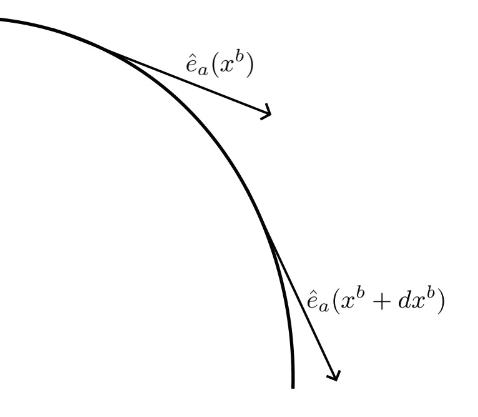
\includegraphics[width=7cm]{figura81.png}
	\caption{ Cambio en los vectores direccionales.}
	\label{fig2112}
\end{figure}


\begin{eqnarray} \nonumber
d\vec{e_a} &=& \vec{e_a}(x^b+dx^b)- \vec{e_a}(x^b) \\ \nonumber
&=&\frac{\partial \vec{e_a}}{\partial x^1}dx^1 +
\frac{\partial \vec{e_a}}{\partial x^2}dx^2 +
\frac{\partial \vec{e_a}}{\partial x^3}dx^3 \\ \label{2.76}
&=& \displaystyle \sum_{b=1}^3 \frac{\partial \vec{e_a}}{\partial x^b}dx^b
\end{eqnarray}



Notemos que el vector $\displaystyle\frac{\partial \vec{e_a}}{\partial x^b}$
se puede escribir como una combinación lineal de los vectores base $\{ \vec{e_a} \}_{a=1}^3$. Es decir

\begin{eqnarray} \nonumber
\frac{\partial \vec{e_1}}{\partial x^1} &=& \alpha_1 \vec{e_1}+ \alpha_2 \vec{e_2} + \alpha_3 \vec{e_3}= \displaystyle\sum_{c=1}^3  \alpha^c \vec{e_c}=\sum_{c=1}^3 \Gamma_{11}^c \vec{e_c} \\ \nonumber
\frac{\partial \vec{e_1}}{\partial x^2} &=& \beta_1 \vec{e_1}+ \beta_2 \vec{e_2} + \beta_3 \vec{e_3}= \displaystyle\sum_{c=1}^3  \beta^c \vec{e_c}=\sum_{c=1}^3 \Gamma_{12}^c \vec{e_c} \\ \nonumber
\frac{\partial \vec{e_1}}{\partial x^3} &=& \gamma_1 \vec{e_1}+ \gamma_2 \vec{e_2} + \gamma_3 \vec{e_3}= \displaystyle\sum_{c=1}^3  \gamma^c \vec{e_c}=\sum_{c=1}^3 \Gamma_{13}^c \vec{e_c} \\ \nonumber
\frac{\partial \vec{e_2}}{\partial x^1} &=& \lambda_1 \vec{e_1}+ \lambda_2 \vec{e_2} + \lambda_3 \vec{e_3}= \displaystyle\sum_{c=1}^3  \lambda^c \vec{e_c}=\sum_{c=1}^3 \Gamma_{21}^c \vec{e_c} \\ \nonumber
 \vdots
 \end{eqnarray}

En resumen 


\begin{equation} \label{2.77}
\frac{\partial \vec{e_a}}{\partial x^b} = \displaystyle\sum_{c=1}^3 \Gamma_{ab}^c \vec{e_c}
\end{equation}

Donde las cantidades $\Gamma_{ab}^c$ son llamadas \underline{Símbolos de Christoffel}. \\
\\
\textbf{\textit{Proposición}:} Los símbolos de Christoffel satisfacen la propiedad de simetría 

\begin{equation} \label{2.78}
\Gamma_{ab}^c = \Gamma_{ba}^c
\end{equation}

\underline{Demostración}: \\
\\


Notemos que 

\begin{eqnarray} \nonumber
\frac{\partial \vec{e_a}}{\partial x^b}&=& \frac{\partial}{\partial x^b} \frac{\partial \vec{x}}{\partial x^a} \\ \nonumber
&=& \frac{\partial}{\partial x^a} \frac{\partial \vec{x}}{\partial x^b} \\ \label{2.79}
&=& \frac{\partial \vec{e_b}}{\partial x^a}  
\end{eqnarray}

Usando \eqref{2.77}

\begin{eqnarray} \nonumber
\displaystyle\sum_{c=1}^3 \Gamma_{ab}^c \vec{e_c}=\displaystyle\sum_{c=1}^3 \Gamma_{ba}^c \vec{e_c} \\ \nonumber
\Leftrightarrow \displaystyle\sum_{c=1}^3 (\Gamma_{ab}^c - \Gamma_{ba}^c ) \vec{e_c} =0
\end{eqnarray}


Como los vectores $\displaystyle \{ \vec{e_a}\}_{a=1}^3$ son linealmente independientes se tiene 

\begin{equation} \label{2.80}
\Gamma_{ab}^c = \Gamma_{ba}^c
\end{equation}

Por tanto los símbolos de Christoffel son simétricos bajo el intercambio de los indices $"a"$ y $"b"$. \\
\\
\\
\textbf{\textit{Teorema:}} Los símbolos de Christoffel satisfacen

\begin{equation} \label{2.81}
\Gamma_{ab}^c = \frac{1}{2} \displaystyle\sum_{c=1}^3 g^{cd} \left( \frac{\partial g_{ad}}{\partial x^b} + \frac{\partial g_{db}}{\partial x^a} - \frac{\partial g_{ab}}{\partial x^d} \right) 
\end{equation}

\underline{Demostración}: \\
\\

Multiplicando \eqref{2.77} por $\displaystyle \vec{e_d}$ se obtiene

	
\begin{eqnarray} \nonumber
\frac{\partial \vec{e_a}}{\partial x^b} \cdot \vec{e_d} &=& \displaystyle\sum_{c=1}^3 \Gamma_{ab}^c \vec{e_c}\cdot \vec{e_d} \\ \nonumber
\frac{\partial}{\partial x^b}(\vec{e_a}\cdot \vec{e_d})- \vec{e_a} \cdot \frac{\partial \vec{e_d}}{\partial x^b} &=& \displaystyle\sum_{c=1}^3 \Gamma_{ab}^c g_{cd} \\ \nonumber
\frac{\partial g_{ad}}{\partial x^b}- \vec{e_a} \cdot \frac{\partial \vec{e_d}}{\partial x^b} &=& \displaystyle\sum_{c=1}^3 \Gamma_{ab}^c g_{cd} 
\end{eqnarray}

Usando \eqref{2.77}

\begin{eqnarray} \nonumber
\frac{\partial g_{ad}}{\partial x^b}- \vec{e_a} \cdot \displaystyle\sum_{c=1}^3 \Gamma_{db}^c \vec{e_c}  &=& \displaystyle\sum_{c=1}^3 \Gamma_{ab}^c g_{cd} \\  \label{2.82}
\frac{\partial g_{ad}}{\partial x^b} &=& \displaystyle\sum_{c=1}^3 \Gamma_{db}^c g_{ca}  + \displaystyle\sum_{c=1}^3 \Gamma_{ab}^c g_{cd} 
\end{eqnarray}

Luego, utilizando \eqref{2.82} calculamos la expresión


\begin{eqnarray*}
\frac{\partial g_{ad}}{\partial x^b} + \frac{\partial g_{db}}{\partial x^a} -\frac{\partial g_{ab}}{\partial x^d} &=& \lefteqn{ \displaystyle\sum_{c=1}^3 \Gamma_{db}^c g_{ca}  + \displaystyle\sum_{c=1}^3 \Gamma_{ab}^c g_{cd} +
 \displaystyle\sum_{c=1}^3 \Gamma_{ad}^c g_{cb}  + \displaystyle\sum_{c=1}^3 \Gamma_{ba}^c g_{cd} } \\
&& - \displaystyle\sum_{c=1}^3 \Gamma_{ad}^c g_{cb}  - \displaystyle\sum_{c=1}^3 \Gamma_{bd}^c g_{ca} \\
&=&  \sum_{c=1}^3 \left( \Gamma_{ab}^c + \Gamma_{ba}^c \right)g_{cd}
+\sum_{c=1}^3 \left( \Gamma_{db}^c - \Gamma_{bd}^c \right)g_{ca}
+\sum_{c=1}^3 \left( \Gamma_{da}^c + \Gamma_{ad}^c \right)g_{cb} \\
\Leftrightarrow \frac{\partial g_{ad}}{\partial x^b} + \frac{\partial g_{db}}{\partial x^a} -\frac{\partial g_{ab}}{\partial x^d}&=& 2 \displaystyle\sum_{c=1}^3 \Gamma_{ab}^c g_{cd} \\
\displaystyle\sum_{c=1}^3 \Gamma_{ab}^c g_{cd} &=& \frac{1}{2} \left( \frac{\partial g_{ad}}{\partial x^b} + \frac{\partial g_{db}}{\partial x^a} -\frac{\partial g_{ab}}{\partial x^d} \right) / \cdot \displaystyle\sum_{d=1}^3 g^{ed} \\
\displaystyle\sum_{d=1}^3 \sum_{c=1}^3 g^{ed} \Gamma_{ab}^c g_{cd} &=& \frac{1}{2} \displaystyle\sum_{d=1}^3 g^{ed}  \left( \frac{\partial g_{ad}}{\partial x^b} + \frac{\partial g_{db}}{\partial x^a} -\frac{\partial g_{ab}}{\partial x^d} \right) \\
\displaystyle\sum_{c=1}^3 \Gamma_{ab}^c \sum_{d=1}^3 g_{cd}g^{ed} &=& \frac{1}{2} \displaystyle\sum_{d=1}^3 g^{ed}  \left( \frac{\partial g_{ad}}{\partial x^b} + \frac{\partial g_{db}}{\partial x^a} -\frac{\partial g_{ab}}{\partial x^d} \right) \\
\displaystyle\sum_{c=1}^3 \Gamma_{ab}^c \displaystyle\delta_c^e &=& \frac{1}{2} \displaystyle\sum_{d=1}^3 g^{ed}  \left( \frac{\partial g_{ad}}{\partial x^b} + \frac{\partial g_{db}}{\partial x^a} -\frac{\partial g_{ab}}{\partial x^d} \right) \\
\Gamma_{ab}^e &=& \frac{1}{2} \displaystyle\sum_{d=1}^3 g^{ed}  \left( \frac{\partial g_{ad}}{\partial x^b} + \frac{\partial g_{db}}{\partial x^a} -\frac{\partial g_{ab}}{\partial x^d} \right). \\ 
\end{eqnarray*}



\textbf{Ejemplo:} Coordenadas esféricas\\


Hay dos formas de calcular los símbolos de Christoffel. La primera es derivar los vectores direccionales con respecto a $r,\phi,\theta$ y la segunda forma es usar la formula \eqref{2.81}. En este caso usaremos la formula para calcular algunos, para ello usaremos la métrica y su inversa

\begin{equation} \nonumber
\Gamma_{11}^c= \frac{1}{2} \displaystyle\sum_{d=1}^3 g^{cd}  \left( \frac{\partial g_{1d}}{\partial r} + \frac{\partial g_{d1}}{\partial r} -\frac{\partial g_{11}}{\partial x^d} \right)
\end{equation}

Considerando que $g_{1d}=g_{d1}$

\begin{equation} \nonumber
\Gamma_{11}^c = \displaystyle\sum_{d=1}^3 g^{cd} \frac{\partial g_{1d}}{\partial r}= g^{c1} \frac{\partial g_{11}}{\partial r} = 0
\end{equation}

Por tanto 

\begin{equation} \label{2.83}
\Gamma_{11}^1= \Gamma_{11}^2 = \Gamma_{11}^3 = 0  
\end{equation}



\begin{eqnarray} \nonumber
\Gamma_{12}^2 &=& \frac{1}{2} \displaystyle\sum_{d=1}^3 g^{2d}  \left( \frac{\partial g_{1d}}{\partial \phi} + \frac{\partial g_{d2}}{\partial r} -\frac{\partial g_{12}}{\partial x^d} \right) \\ \nonumber
&=& \frac{1}{2} g^{22} \left( \frac{\partial g_{12}}{\partial \phi} + \frac{\partial g_{22}}{\partial r} \right) \\ \nonumber
&=& \frac{1}{2r^2 \sin^2 \theta} \frac{\partial}{\partial r} \left(r^2 \sin^2 \theta \right) \\ \nonumber
&=& \frac{1}{r}
\end{eqnarray}

Por tanto 

\begin{equation}\label{2.84}
\Gamma_{12}^2= \frac{1}{r}.
\end{equation}



\begin{eqnarray} \nonumber
\Gamma_{22}^3 &=& \frac{1}{2} \displaystyle\sum_{d=1}^3 g^{3d}  \left( \frac{\partial g_{2d}}{\partial \phi} + \frac{\partial g_{d2}}{\partial \phi} -\frac{\partial g_{22}}{\partial x^d} \right) \\ \nonumber
&=&-\frac{1}{2} g^{33}\frac{\partial g_{22}}{\partial \theta} \\ \nonumber
&=& - \frac{1}{2r^2} \frac{\partial}{\partial \theta} \left( r^2 \sin^2 \theta \right) \\ \nonumber
&=& -\sin \theta \cos \theta
\end{eqnarray}


Por tanto

\begin{equation} \label{2.85}
\Gamma_{22}^3=-\sin \theta \cos \theta.
\end{equation}
\\


\begin{itemize}
 \item \underline{\textbf{Nota Historica}} \\
\end{itemize}


 Los simbolos que estudiamos aquí fueron introducidos en la matemática, a finales del sigo XIX, por el alemán Elwin Bruno Christoffel (1829-1900), que fue , junto con Bernard Riemann, el primero en establecer la noción de Tensor, y, en la practica, el creador del luego llamado Cálculo Tensorial.






\section{Transformación de Coordenadas}

Como ya hemos mencionado con anterioridad, es muy importante elegir un sistema de coordenadas adecuado con el objetivo de simplificar las ecuaciones y hacer mas fácil la resolución de problemas. Para ello es fundamental conocer las relaciones entre los diferentes sistemas coordenados, por lo que dedicaremos esta sección a interiorizarnos un poco en las \textit{transformaciones de coordenadas}. \\ 



\textbf{Ejemplo:} Un caso que ya hemos estudiado anteriormente es la conversión de coordenadas cartesianas a esféricas:

\begin{eqnarray} \nonumber
x(r,\phi,\theta) &=& r \cos{\phi} \sin{\theta} \\ \nonumber
y(r,\phi,\theta) &=& r \sin{\phi} \sin{\theta} \\ \nonumber
z(r,\phi,\theta) &=& r \cos{\theta}.
\end{eqnarray}


En general una transformación de coordenadas esta dada por la relación

\begin{eqnarray} \nonumber
O x^1 x^2 x^3 &\longrightarrow& O' x^{1'} x^{2'} x^{3'} \\ \nonumber
x^a &\longrightarrow& x^{a'}
\end{eqnarray}

\begin{figure}[h]
	\centering
	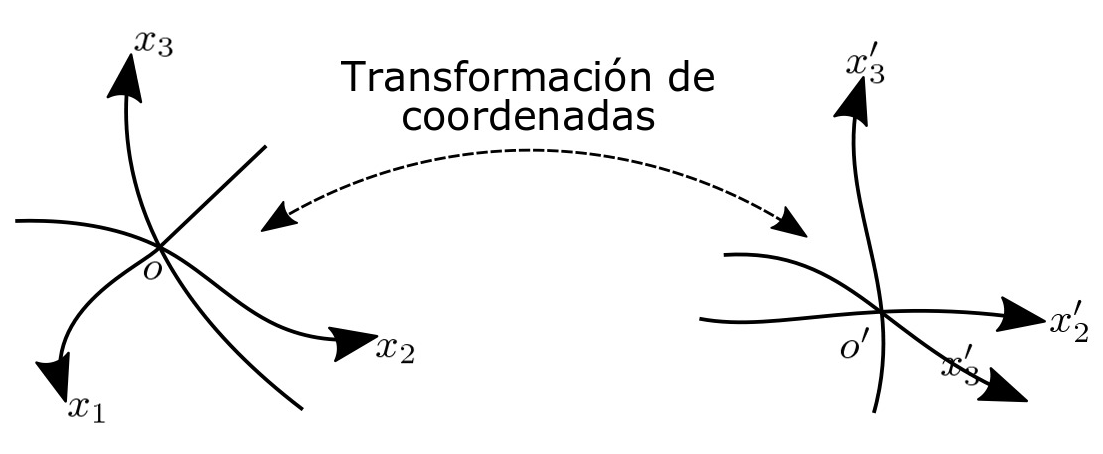
\includegraphics[width=12cm]{figura133.png}
	\caption{ Transformación de coordenadas.}
	\label{}
\end{figure}



donde:

\begin{eqnarray} \nonumber
x^1= x^1(x^{1'},x'^{2},x'^{3}) \\ \nonumber
x^2= x^2(x^{1'},x'^{2},x'^{3}) \\ \nonumber
x^3= x^3(x^{1'},x'^{2},x'^{3}).
\end{eqnarray}


La transformación $x^a(x'^{b})$ debe ser invertible, es decir, el determinante de la matriz Jacobiana debe ser distinto de cero. \\

Consideremos la matriz Jacobiana

\begin{eqnarray}
\frac{\partial \left(x^1, x^2, x^3 \right)}{ \partial \left( x'^{1}, x'^{2},x'^{3} \right)}
&=&
\left(
\begin{array}{ccc} \nonumber
\displaystyle\frac{\partial x^1}{\partial x'^1} & \displaystyle\frac{\partial x^1}{\partial x'^2} & \displaystyle\frac{\partial x^1}{\partial x'^3} \\ \nonumber
\displaystyle\frac{\partial x^2}{\partial x'^1} & \displaystyle\frac{\partial x^2}{\partial x'^2} & \displaystyle\frac{\partial x^2}{\partial x'^3} \\ \nonumber
\displaystyle\frac{\partial x^3}{\partial x'^1} & \displaystyle\frac{\partial x^3}{\partial x'^2} & \displaystyle\frac{\partial x^3}{\partial x'^3}
\end{array}
\right) \\ \nonumber
\\ \nonumber
 &=& \frac{\partial x^a}{\partial x'^b} \\ \label{2.86}
 &=&J^a_{ \ b}
\end{eqnarray}

luego, el determinante de la matriz Jacobiana debe ser distinto de cero

\begin{equation} \label{2.87}
\det{J^a_{\ b }} \neq 0
\end{equation}


\textbf{Ejemplo:} Coordenadas esféricas 


\begin{equation}
O x,y,z \longrightarrow Or,\phi,\theta \nonumber
\end{equation}


En este caso la matriz Jacobiana esta dada por:

\begin{eqnarray} \nonumber
J^a_{\ b}
=
\left(
\begin{array}{ccc}
\displaystyle\frac{\partial x}{\partial r} & \displaystyle\frac{\partial x}{\partial \phi} & \displaystyle\frac{\partial x}{\partial \theta} \\
\displaystyle\frac{\partial y}{\partial r} & \displaystyle\frac{\partial x^y}{\partial \phi} & \displaystyle\frac{\partial y}{\partial \theta} \\
\displaystyle\frac{\partial z}{\partial r} & \displaystyle\frac{\partial z}{\partial \phi} & \displaystyle\frac{\partial z}{\partial \theta}
\end{array}
\right)
\end{eqnarray} 


luego:

\begin{equation} \label{2.88}
\det{J^a_{\ b}}=r^2 \sin{\theta} \neq 0
\end{equation}

notemos que cuando $r=0$ y $\theta=0,\pi,...$ la transformación no esta definida y falla. \\


\textbf{\textit{Proposición:}}  Los vectores direccionales $e_a$ y $e'_a$ estan relacionados por la formula

\begin{equation} \label{2.89}
\vec{e}_a = \sum_{b=1}^3 \frac{\partial x'^b}{\partial x^a} \vec{e}\ '_{b}
\end{equation}


\textbf{Demostración:} 

\begin{eqnarray} \nonumber
\vec{e}_a = \frac{\partial x(x^b)}{\partial x^a}&=&\frac{\partial x(x^b(x'^c)}{\partial x^a} \\ \nonumber
&=&\frac{\partial y(x'^b)}{\partial x^a} \\ \nonumber
&=&\sum_{b=1}^3 \frac{\partial y}{\partial x'^b}\frac{\partial x'^b}{\partial x^a} \\ \nonumber
\vec{e}_a&=&\sum_{b=1}^3 \frac{\partial x'^b}{\partial x^a} \vec{e}\ '_{b}
\end{eqnarray}



Si la transformación es invertible podemos obtener $\vec{e}\ '_a$ en función de $\vec{e}_a$, es decir

\begin{eqnarray} \nonumber
\sum_{b=1}^3 \frac{\partial x^b}{\partial x'a} \vec{e}_b&=&\sum_{b=1}^3 \frac{\partial x^b}{\partial x'^a} \sum_{c=1}^3 \frac{\partial x'^c}{\partial x^b} \vec{e}\ '_c \\ \nonumber
&=&\sum_{b=1}^3 \sum_{c=1}^3\frac{\partial x^b}{\partial x'^a}  \frac{\partial x'^c}{\partial x^b} \vec{e}\ '_c \\ \nonumber
&=&\sum_{c=1}^3 \frac{\partial x'^c}{\partial x^a} \vec{e}\ _c ' \\ \nonumber
&=& \vec{e}\ '_a
\end{eqnarray}

\textbf{\textit{Proposición:}} Las componentes del vector $\vec{A}$ en $O x^1,x^2,x^3$ y en $O'x'^1,x'^2,x'^3$ están relacionadas mediante


\begin{equation} \label{2.90}
A'^a = \sum_{b=1}^3 \frac{\partial x'^a}{\partial x^b}A^b
\end{equation}


\textbf{\textit{Proposición:}} La métrica $g_{ab}$ en el sistema $O x^1,x^2,x^3$ transforma al sistema de coordenadas $O'x'^1,x'^2,x'^3$ como

\begin{equation} \label{2.91}
g'_{ab}= \sum_{c=1}^3 \sum_{d=1}^3 \frac{\partial x^c}{\partial x'^a}\frac{\partial x^d}{\partial x'^b} g_{cd}
\end{equation}


Dejamos como ejercicio demostrar estas dos ultimas proposiciones. 

\section{Cinematica de una Particula }


En las secciones anteriores nos dedicamos a realizar un estudio puramente geométrico, principalmente centrado en un punto P situado en el espacio y representado por su vector de posición, el cual representaríamos mediante un sistema de coordenadas. A continuación nos ocuparemos de estudiar la posición de una partícula a medida que pasa el tiempo, considerando características asociadas al movimiento, tales como la velocidad y la aceleración. Si $\vec{x}$ es el vector posición de nuestro punto de interés, entonces $\vec{x}=\vec{x}(t)$


\subsection{Velocidad}

 
La velocidad es la variación de la posición en el tiempo, la cual podemos estudiar mediante un proceso limite.


\begin{equation} \label{2.92}
\vec{v}=\lim_{\epsilon \to 0} \frac{\vec{x}(t+\epsilon)-\vec{x}(t)}{\epsilon}=\frac{d\vec{x}}{dt}
\end{equation}


\begin{figure}[H]
	\begin{center}
	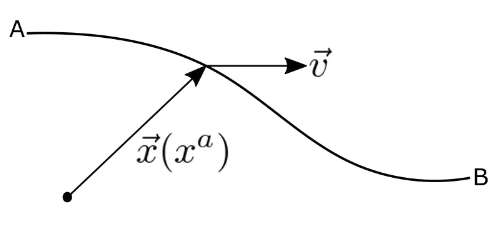
\includegraphics[width=7cm]{figura101.png}
	\caption{ Velocidad.}
	\label{fig.1}
	\end{center}
\end{figure}



Considerando que $\displaystyle\vec{v}=\frac{d\vec{x}(x^a)}{dt}$

\begin{eqnarray} \nonumber
\vec{v} &=& \frac{d\vec{x}(x^a)}{dt} = \frac{\partial \vec{x}}{\partial x^1}\frac{dx^1}{dt} + \frac{\partial \vec{x}}{\partial x^2}\frac{dx^2}{dt} + \frac{\partial \vec{x}}{\partial x^3}\frac{dx^3}{dt} \\ \nonumber
\vec{v} &=& \sum_{a=1}^3 \frac{\partial \vec{x}}{\partial x^a}\frac{dx^a}{dt} = \sum_{a=1}^3\frac{dx^a}{dt} \vec{e}_a \\ \nonumber
\vec{v} &=& \sum_{a=1}^3 v^a \vec{e}_a  
\end{eqnarray}

donde

\begin{equation} \label{2.93}
v^a=\frac{dx^a}{dt}
\end{equation}

y ademas

\begin{equation} \label{2.94}
v := \norm{\vec{v}} = \sqrt{\vec{v}\cdot \vec{v}} = \sum_{a=1}^3\sum_{b=1}^3 g_{ab}v^av^b
\end{equation}



\subsection{$\vec{v}$ en coordenadas cartesianas}


\begin{equation}\nonumber
\vec{e}_1= \hat{\imath} \ \ \  \ \ \ \vec{e}_2= \hat{\jmath} \ \ \  \ \ \ \vec{e}_3= \hat{k}
\end{equation}

\begin{equation} \nonumber
x^1=x \ \ \  \ \ \ x^2=y \ \ \  \ \ \ x^3=z
\end{equation}


El vector velocidad esta dado por 

\begin{equation} \label{2.95}
\vec{v}=\frac{dx}{dt}\hat{\imath} + \frac{dx}{dt}\hat{\jmath} + \frac{dx}{dt} \hat{k}
\end{equation}

Entonces

\begin{equation} \label{2.96}
v^1= \frac{dx}{dt} \ \ \ , \ \ \ v^2=\frac{dy}{dt} \ \ \ , \ \ \ v^3=\frac{dz}{dt}
\end{equation}









\subsection{$\vec{v}$ en coordenadas cilindricas}

\begin{eqnarray} \nonumber
\vec{v}&=&\frac{d\vec{x}}{dt} = \frac{d}{dt} \left( r\hat{r} + \phi r \hat{\phi} + z \hat{z} \right) \\\nonumber
\vec{v} &=& \frac{dr}{dt} \hat{r} + r\frac{d\phi}{dt} \hat{\phi} + \frac{dz}{dt} \hat{z} \\ \label{2.97}
&=& \frac{dr}{dt} \vec{e}_1 + \frac{d\phi}{dt} \vec{e}_2 + \frac{dz}{dt} \vec{e}_3
\end{eqnarray}

Entonces

\begin{equation} \label{2.98}
v^1 = \frac{dr}{dt} \ \ \ , \ \ \  v^2 = \frac{d\phi}{dt} \ \ \ , \ \ \  v^3 = \frac{dz}{dt}.
\end{equation}


\subsection{Relacion entre $v$ y $ds$}


Anteriormente hemos deducido una relación entre la métrica y el elemento de linea la cual esta dada por \eqref{2.47} 


\begin{eqnarray} \nonumber
ds^2 &=&  \sum_{a=1}^3 \sum_{b=1}^3 g_{ab} dx^a dx^b \\ \label{2.99}
ds &=& \sqrt{\sum_{a=1}^3 \sum_{b=1}^3 g_{ab} dx^a dx^b }
\end{eqnarray}


pero, en este caso debemos considerar que 

\begin{eqnarray} \nonumber
x^a = x^a(t) 
\end{eqnarray}

y 

\begin{equation} \label{2.100}
dx^a=\frac{dx^a}{dt}dt = v^a dt
\end{equation}

Luego, reemplazando \eqref{2.100} en \eqref{2.99}

\begin{eqnarray} \nonumber
ds &=& \sqrt{\sum_{a=1}^3 \sum_{b=1}^3 g_{ab} v^a v^b (dt)^2 } = \sqrt{\sum_{a=1}^3 \sum_{b=1}^3 g_{ab} v^a v^b }  dt \\
ds &=& vdt 
\end{eqnarray}
 
 Entonces,
 
 
\begin{equation} \label{2.102}
\Delta s = \displaystyle\int_{t_1}^{t_2} vdt.
\end{equation}



\subsection{Aceleración}

La aceleración es la variación de la velocidad en el tiempo, es decir 


\begin{eqnarray} \nonumber
\vec{a}&=&\frac{d\vec{v}}{dt} = \frac{d}{dt} \left( \sum_{a=1}^3 v^a  \vec{e}_a \right) \\ \label{2.103}
\vec{a} &=& \sum_{a=1}^3 \left( \frac{dv^a}{dt}\vec{e}_a + v^a \frac{d\vec{e}_a}{dt} \right)
\end{eqnarray}


Recordemos que los vectores direccionales presentan una dependencia temporal, es decir, $\vec{e}_a = \vec{e}_a (x^b)= \vec{e}_a (x^b(t))$ . Entonces  se tiene que 

\begin{eqnarray} \label{2.104}
\frac{d\vec{e}_a}{dt} = \sum_{b=1}^3 \frac{\partial \vec{e}_a}{\partial x^b} \frac{dx^b}{dt}= \sum_{b=1}^3 \sum_{c=1}^3 \Gamma_{ab}^c v^b \vec{e}_c
\end{eqnarray}

Luego, reemplazando \eqref{2.104} en \eqref{2.103} se obtiene

\begin{eqnarray} \nonumber
\vec{a} &=& \sum_{a=1}^3 \left( \frac{dv^a}{dt}\vec{e}_a + v^a \sum_{b=1}^3 \sum_{c=1}^3 \Gamma_{ab}^c v^b \vec{e}_c  \right) \\ \nonumber
&=& \sum_{a=1}^3  \frac{dv^a}{dt}\vec{e}_a + \sum_{a=1}^3 \sum_{b=1}^3 \sum_{c=1}^3 \Gamma_{ab}^c v^a v^b \vec{e}_c 
\end{eqnarray}


Con el objetivo de representar de forma mas clara este resultado, realizamos un intercambio en los indices de suma

\begin{eqnarray} \nonumber
\vec{a} &=& \sum_{a=1}^3  \frac{dv^a}{dt}\vec{e}_a + \sum_{a=1}^3 \sum_{b=1}^3 \sum_{c=1}^3 \Gamma_{ab}^c v^a v^b \vec{e}_c  \\ \nonumber
&=& \sum_{a=1}^3  \frac{dv^a}{dt}\vec{e}_a + \sum_{b=1}^3 \sum_{c=1}^3 \sum_{a=1}^3 \Gamma_{bc}^a v^c v^b \vec{e}_a \\ \nonumber
&=& \sum_{a=1} \left( \frac{dv^a}{dt} + \sum_{b}^3 \sum_{c}^3 \Gamma_{bc}^a v^b v^c \right) \vec{e}_a \\ \label{2.105}
&=& \sum_{a=1}^3 a^a \vec{e}_a 
\end{eqnarray}

Por tanto

\begin{eqnarray} \label{2.106}
a^a = \frac{dv^a}{dt} + \sum_{b}^3 \sum_{c}^3 \Gamma_{bc}^a v^b v^c
\end{eqnarray}


o tambien

\begin{equation} \label{2.107}
a^a = \frac{d^2x^a}{dt^2} + \sum_{b}^3 \sum_{c}^3 \Gamma_{bc}^a \frac{dx^b}{dt} \frac{dx^c}{dt}.
\end{equation}
\\

\subsection{$\vec{a}$ en coordenadas cartesianas}

En coordenadas cartesianas

\begin{equation} \nonumber
g_{ab}=\delta_{ab} \Rightarrow \Gamma_{ab}^c = 0
\end{equation}

por tanto 

\begin{equation} \nonumber
a^a = \frac{d^2 x}{dt^2}= \frac{dv^a}{dt}
\end{equation}

Luego,

\begin{equation} \nonumber
a^1 = \frac{dv^1}{dt} \ \ \ \ \  \ a^2 = \frac{dv^2}{dt} \ \ \ \ \ \ \ a^3 = \frac{dv^3}{dt}
\end{equation}


\subsection{$\vec{a}$ en coordenadas cilindricas}

En este caso nos sera útil considerar los vectores direccionales en coordenadas cilíndricas los cuales  están dados por

\begin{equation} \nonumber
\vec{e}_1= \hat{r} \ \ \  \ \ \ \ \vec{e}_2 = r\hat{\phi} \ \ \ \ \ \ \vec{e}_3= \hat{k}
\end{equation}

utilizando \eqref{2.81} podemos calcular los símbolos de Christoffel. A continuación veremos los casos en los cuales los símbolos son distintos de cero, queda como ejercicio verificar que en el resto de las situaciones resulta cero. \\

Utilizando \eqref{2.81} consideremos los siguientes casos \\

\begin{itemize}
\item $a=1 \ \ \ b=2 \ \ \ $
\end{itemize}

\begin{eqnarray} \nonumber
\frac{\partial \vec{e}_1}{\partial \phi} &=&  \hat{\phi}=\frac{1}{r}\vec{e}_2 \\ \nonumber
\Rightarrow  \sum_{c=1}^3 \Gamma_{12}^c &=& \Gamma_{12}^1\vec{e}_1 + \Gamma_{12}^2\vec{e}_1 + \Gamma_{12}^3\vec{e}_1 = \frac{1}{r} \vec{e}_2
\end{eqnarray}

Por tanto

\begin{equation} \nonumber
\Gamma_{12}^1=0 \ \ \ \ \ \ \Gamma_{12}^1=\frac{1}{r} \ \ \ \ \ \ \Gamma_{12}^1=0
\end{equation}



\begin{itemize}
\item $a=2 \ \ \ b=1 \ \ \ $
\end{itemize}


\begin{eqnarray} \nonumber
\frac{\partial \vec{e}_2}{\partial r} &=&  \frac{1}{r} \vec{e}_2 \\ \nonumber
\Rightarrow \Gamma_{21}^2 &=& \frac{1}{r}
\end{eqnarray}

Por otra parte

\begin{equation} \nonumber
\Gamma_{21}^1=0 \ \ \ \ \ \ \Gamma_{21}^3=0 
\end{equation}

Una forma mas rápida para obtener $\Gamma_{21}^2$, es argumentar la igualdad con el caso anterior mediante la propiedad de simetría dada en \eqref{2.78}

\begin{itemize}
\item $a=2 \ \ \ b=2 \ \ \ $
\end{itemize}

\begin{eqnarray} \nonumber
\frac{\partial \vec{e}_2}{\partial \phi} &=& -r \vec{e}_1  \\ \nonumber
\Rightarrow  \sum_{c=1}^3 \Gamma_{22}^c &=& \Gamma_{22}^1\vec{e}_1 + \Gamma_{22}^2\vec{e}_1 + \Gamma_{22}^3\vec{e}_1 = -r \vec{e}_1
\end{eqnarray}

Por tanto

\begin{equation} \nonumber
\Gamma_{22}^1=-r \ \ \ \ \ \ \Gamma_{22}^2= 0 \ \ \ \ \ \ \Gamma_{22}^3=0.
\end{equation}	
\\


Luego, reemplazando estos valores en \eqref{2.105} obtenemos

\begin{eqnarray} \nonumber
\vec{a} &=& \frac{d^2r}{dt^2} \vec{e}_1 + \frac{dr}{dt} \frac{d\phi}{dt} \frac{1}{r} \vec{e}_2 + \frac{d^2\phi}{dt^2} \vec{e}_2 + \frac{dr}{dt} \frac{d\phi}{dt} \frac{1}{r} \vec{e}_2 - r\left(\frac{d\phi}{dt}  \right)^2 \vec{e}_1  + \frac{d^2 z}{dt^2} \vec{e}_3 \\ \nonumber
&=& \left( \ddot{r}- r \dot{\phi}^2 \right)\vec{e}_1 + \left( \frac{2}{r} \dot{r} \dot{\phi} + \ddot{\phi}  \right)\vec{e}_2 + \ddot{z} \vec{e}_3 \\ \label{108}
\vec{a} &=& \left( \ddot{r}- r \dot{\phi}^2 \right)\hat{r} + \left( 2 \dot{r} \dot{\phi} + r\ddot{\phi}  \right)\hat{\phi} + \ddot{z} \hat{k}.  
\end{eqnarray}

























 

\chapter{Fuerzas Centrales}\label{chapter3}


Una fuerza central es aquella en que la fuerza es paralela o antiparalela al vector posición, es decir, de la forma 

\begin{equation} \label{3.1}
\vec{F}= f(r)\hat{r}.
\end{equation}

\textbf{\textit{Teorema:}} Una fuerza central genera un movimiento planar. \\
\\
\textbf{Demostración}: Considerando  que $\vec{r}=r\hat{r}$ y $\vec{F}=f(r)\hat{r}$

\begin{eqnarray} \nonumber
\vec{\tau}_0=r\hat{r} \times f(r)\hat{r}&=&rf(r)\hat{r} \times \hat{r}=0 \\ \nonumber
\Rightarrow \vec{\tau}_0 = \frac{d\vec{L}_0}{dt}&=&0 \\ \nonumber
\Rightarrow \vec{L}_{0} &=& cte
\end{eqnarray}

\begin{figure}[H]
	\begin{center}
	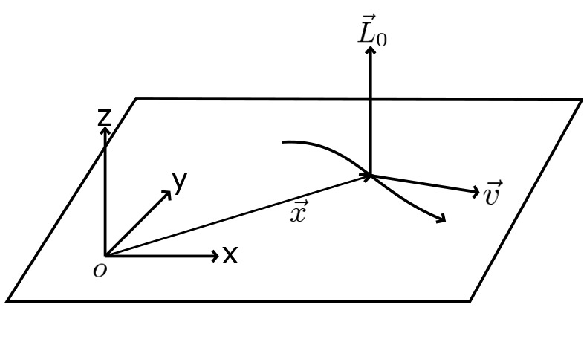
\includegraphics[width=8cm]{figura11.png} 
	\caption{ Momento angular asociado a una fuerza central}
	\label{fig.1}
	\end{center}
\end{figure}

Puesto que $\vec{L}_0$ es constante, $\vec{r}$ y $\vec{p}$ están  permanentemente contenidos en un plano perpendicular a $\vec{L}_0$. Por tanto la fuerza central genera un movimiento planar. \\
\\


\textbf{\textit{Teorema:}} Las fuerzas centrales son conservativas. \\
\\

 \textit{Demostración}: De \eqref{1.6} sabemos que si una fuerza es conservativa entonces $\displaystyle \vec{\nabla} \times \vec{F} =0$. En este caso se tiene que $\vec{F}=f(r)\hat{r}$, luego
 
\begin{eqnarray}
\vec{\nabla} \times \vec{F}=
\left|
\begin{array}{ccc}
 \hat{r} & r\hat{\phi} & 0 \\ \\
\displaystyle\frac{\partial}{\partial r} & \displaystyle\frac{\partial }{\partial \theta} & 0 \\ \\
 f(r) & 0 & 0
\end{array}
\right|
=0
\end{eqnarray}
 
 Por tanto las fuerzas centrales son conservativas. \\
 \\
 
 \textbf{\textit{Teorema:}} Si un movimiento central se conserva la energía mecánica es 
 
\begin{equation}
E=K+U=cte
\end{equation}

\section{Principio de Conservación de la Energía y el Momento Angular}

Un punto importante en nuestro análisis es encontrar y estudiar las ecuaciones del movimiento asociadas a un movimiento generado por una fuerza central. Para ello consideremos $\vec{F}=f(r)\hat{r}$ en la segunda ley de Newton usando coordenadas cilíndricas.

\begin{eqnarray}
f(r)\hat{r}&=&m \left\{  \left( \ddot{r}- r \dot{\phi}^2 \right)\hat{r} + \left( 2 \dot{r} \dot{\phi} + r\ddot{\phi}  \right)\hat{\phi} + \cancelto{0}{\ddot{z}} \hat{k}  \right\} \\
&=& m  \left( \ddot{r}- r \dot{\phi}^2 \right)\hat{r} + m\left( 2 \dot{r} \dot{\phi} + r\ddot{\phi}  \right)\hat{\phi} 
\end{eqnarray}

donde
\begin{eqnarray} 
\left. \begin{matrix}
m \ddot{r} -mr \dot{\phi}^2 = f(r)   \\ \\ 
m\underbrace{\left(r\ddot{\phi} + 2\dot{r}\dot{\phi}\right)}_{(*)}=0
\end{matrix}\right\} 
\quad \mbox{Ecuaciones del movimiento}
\end{eqnarray} 

De la segunda ecuación notemos que podemos escribir (*) como

\begin{equation}
2\dot{r}\dot{\phi} + r\ddot{\phi} = \frac{1}{r} \left( 2\dot{r}r \dot{\phi} + r^2 \ddot{\phi} \right) = \frac{1}{r} \frac{d}{dt}\left(r^2 \dot{\phi}\right)
\end{equation}

Reemplazando este resultado obtenemos

\begin{eqnarray}
\frac{m}{r}\frac{d}{dt} \left( r^2 \dot{\phi} \right)&=&0 \\
\frac{1}{r} \frac{d}{dt} \left( mr^2 \dot{\phi} \right)&=&0 \\
\Rightarrow \frac{d}{dt} \left( mr^2 \dot{\phi} \right)&=&0
\end{eqnarray}

Considerando que $\vec{L}_0 = mr^2 \dot{\phi} \hat{k}$, la ecuación (3.9) resulta

\begin{equation}
\frac{d L_0}{dt} =0
\end{equation}

Integrando obtenemos

\begin{equation}
L_0 = mr^2 \dot{\phi}=cte. 
\end{equation}
\\



Recordemos que, como la fuerza $\vec{F}=f(r)\hat{r}$ es conservativa, la energía $E$ también se conserva. \\

\begin{eqnarray}
E=\frac{1}{2} m \left( \dot{r}^2 + r^2 \dot{\phi}^2 \right) + U
\end{eqnarray} 

Con el objetivo de desacoplar las variables consideremos (3.11), de aquí obtenemos que 

\begin{equation}
\dot{\phi}^2 = \frac{L_0^2}{m^2 r^4}
\end{equation}

Finalmente, reemplazando en (3.12)

\begin{eqnarray}
E&=&\frac{1}{2}m \left( \dot{r}^2 + r^2 \frac{L_0^2}{m^2 r^4} \right) +  U(r) \\
&=& \frac{1}{2}m\dot{r}^2 +\frac{L_0^2}{2m r^2} +  U(r).
\end{eqnarray}


El termino $\displaystyle V_c=\frac{L_0^2}{2mr^2}$ es conocido como energía potencial asociada a la fuerza centrifuga. \\


\begin{figure}[H]
	\begin{center}
	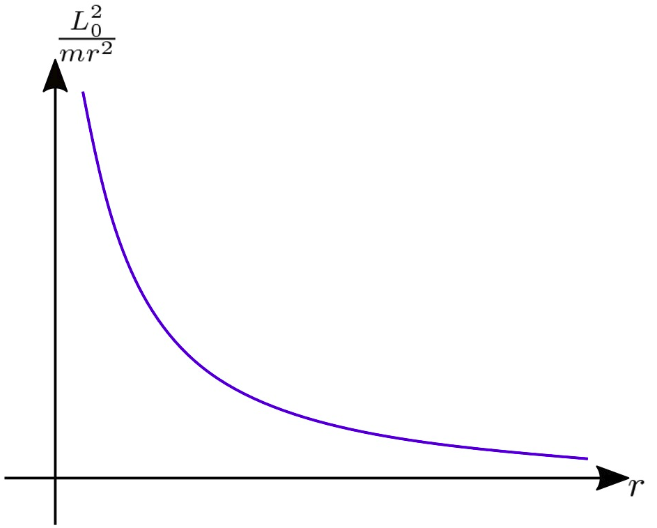
\includegraphics[width=8cm]{figura121.png} 
	\caption{Barrera centrifuga.}
	\label{fig.1}
	\end{center}
\end{figure}



\textbf{\underline{Nota 1}:} La barrera centrifuga $\displaystyle V_c=\frac{L_0^2}{2mr^2}$ es parte de la energía cinética. No es la energía potencial que usualmente trabajamos. \\
\\

\textbf{\underline{Nota 2}:} Para la energía potencial asociada a (3.15) tenemos que

\begin{eqnarray}
f(r)\hat{r} &=& -\vec{\nabla}U(r) \\ 
&=& -\left( \frac{\partial U}{\partial r} \hat{r} + \frac{1}{r} \cancelto{0}{\frac{\partial U}{\partial \phi}} \hat{\phi} \right) \\
&=&- \frac{dU}{dr} \hat{r} \\
\Rightarrow \frac{dU}{dr}&=&-f(r) \\
\Rightarrow U(r)&=&U(r_f) - \int_{r_f}^{r} f(r')dr'.
\end{eqnarray}







\subsection{Potencial efectivo}

Se define el potencial efectivo como:

\begin{equation}
V_{ef}=\frac{L_0^2}{2mr^2 } + U(r).
\end{equation}


Notemos que 

\begin{eqnarray}
&E&= \frac{1}{2}m \dot{r}^2 + V_{ef} \\
&\Rightarrow& \frac{1}{2}m \dot{r}^2 = E-V_{ef} \geq 0 \\
&\Rightarrow& \commentedbox{ E \geq V_{ef}}{}
\end{eqnarray}


\subsection{Ecuaciones paramétricas}

Las ecuaciones paramétricas de la trayectoria para un movimiento producido por una fuerza central son

\begin{eqnarray}
L&=&mr^2 \dot{\phi} \\
E&=&\frac{1}{2}m\dot{r}^2 + V_{ef}
\end{eqnarray}

Resolviendo (3.26) tenemos

\begin{eqnarray}
\dot{r}^2 &=& \frac{2}{m} \left( E - V_{ef} \right) \\
\Rightarrow \frac{dr}{dt}&=& \sqrt{\frac{2}{m} \left( E - V_{ef} \right)} \\
\Rightarrow t&=&\displaystyle \int_{r_0}^{r} \frac{dr}{\sqrt{\frac{2}{m}\left( E-V_{ef} \right)}}
\end{eqnarray}





Por otra parte para  (3.25) 

\begin{eqnarray}
\frac{d\phi}{dt}&=& \frac{L_0}{mr^2} \\
\Rightarrow d\phi&=& \frac{L_0}{mr^2} dt \\
\Rightarrow \phi &=& \phi_0 +\frac{L_0}{m} \int_{0}^{t} \frac{dt}{r^2}
\end{eqnarray}

En resumen:


\begin{eqnarray}
\left.
\begin{matrix}
t&=&\displaystyle \int_{r_0}^{r} \frac{dr}{\sqrt{\frac{2}{m}\left( E-V_{ef} \right)}} \\ \\
\phi &=& \displaystyle \phi_0 +\frac{L_0}{m} \int_{0}^{t} \frac{dt}{r^2} 
\end{matrix}
\right\}
\end{eqnarray}














\section{Ecuación de la Trayectoria}


En esta ocasión nos interesa obtener de forma explicita  una ecuación $r=r(\phi)$ que describa la trayectoria producida por una fuerza central sin considerar el parámetro temporal  

\begin{eqnarray}
\frac{dr}{dt}=\frac{dr}{d\phi} \frac{d\phi}{dt}= \frac{L_o}{mr^2} \frac{dr}{d\phi}
\end{eqnarray}

Luego, reemplazando (3.29) en (3.35)

\begin{eqnarray}
\frac{L_0}{mr^2} \frac{dr}{d\phi} &=& \sqrt{\frac{2}{m} \left( E - V_{ef} \right)} \left/ \right. \cdot m \\
\frac{L_0}{r^2} \frac{dr}{d\phi} &=& \sqrt{2m \left( E-V_{ef} \right)} \\
\Rightarrow d\phi&=& \displaystyle \frac{\displaystyle\frac{L_0}{r^2}}{\sqrt{2m \left( E-V_{ef} \right)}}dr \\
\Rightarrow \phi &=& L_0 \int \displaystyle \frac{\displaystyle\frac{dr}{r^2}}{\sqrt{2m \left( E-V_{ef} \right)}} + C
\end{eqnarray}


utilizando el cambio de variable

\begin{equation}
\chi=\frac{1}{r} \ \ \ , \ \ \  d\chi=-\frac{1}{r^2} dr
\end{equation}

obtenemos

\begin{equation}
\phi(r)=-L_0 \int \frac{d\chi}{\sqrt{2m \left( E-V\left(\frac{1}{\chi}\right) \right)}} + C'
\end{equation}











\section{Ecuación de Binet}

Consideremos la ecuación (3.6) con fuerza central

\begin{equation}
m \ddot{r} -mr \dot{\phi}^2 = f(r)
\end{equation}

la cual, mediante (3.26) podemos escribir como

\begin{equation}
m \left( \ddot{r} - \frac{L_o^2}{m^2 r^3} \right) = f(r)
\end{equation}

Este método consiste en reemplazar $r(t)$ por la ecuación de la trayectoria $r(\phi)$, ya que la ecuación resultante es mas sencilla de resolver que la ecuación original. Para eliminar el tiempo y obtener la dependencia en $\phi$ usamos la regla de la cadena. \\
\\

Sea $r=r(\phi)$, luego

\begin{eqnarray}
\frac{dr}{dt} &=& \frac{dr}{d\phi} \frac{d\phi}{dt} = \dot{\phi} \frac{dr}{d\phi}  \\
\frac{dr}{dt} &=& \frac{L_0}{mr^2} \frac{dr}{d\phi} = - \frac{L_0}{m} \frac{d}{d\phi} \left( \frac{1}{r} \right)
\end{eqnarray}

derivando con respecto al tiempo obtenemos

\begin{eqnarray}
\ddot{r} &=& \frac{d\phi}{dt} \frac{d}{d\phi} \left( \dot{\phi} \frac{dr}{d\phi} \right) = \dot{\phi} \frac{d}{d\phi} \left( -\frac{L_0}{m} \frac{d}{d\phi} \left( \frac{1}{r} \right) \right)  \\
\ddot{r}&=&  -\frac{L_0^2}{m^2 r^2} \frac{d^2}{d\phi^2} \left( \frac{1}{r} \right)  
\end{eqnarray}

Asi, reemplazando (3.47) en (3.43) la fuerza queda expresada como 

\begin{eqnarray}
f(r)&=&m \left[  -\frac{L_0^2}{m^2 r^2} \frac{d^2}{d\phi^2} \left( \frac{1}{r} \right)  - \frac{L_o^2}{m^2 r^3} \right] \\
&=& -m\frac{L_o^2}{m^2 r^2} \left[ \frac{d^2}{d\phi^2} \left( \frac{1}{r} \right) + \frac{1}{r} \right]
\end{eqnarray}

Por tanto

\begin{eqnarray}
\left.
\begin{matrix}
\displaystyle f(r)=-\frac{L_o^2}{m r^2} \left[ \frac{d^2}{d\phi^2} \left( \frac{1}{r} \right) + \frac{1}{r} \right]
\end{matrix}
\right\}
\quad \mbox{Ecuación de Binet}
\end{eqnarray}














\section{Problema de Kepler}


Un ejemplo importante de campo central es aquel en el que la energía potencial es inversamente proporcional a $r$, y, como consecuencia, la fuerza sera inversamente proporcional a $r^2$. Un caso de gran interés para el curso es el campo gravitatorio de Newton. \\


\begin{figure}[H]
	\begin{center}
	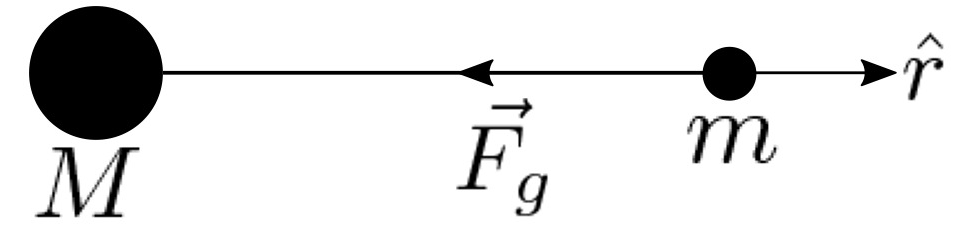
\includegraphics[width=8cm]{figura131.png} 
	\caption{ Fuerza gravitacional.}
	\label{fig.1}
	\end{center}
\end{figure}


De la ley de gravitación universal se tiene

\begin{equation}
\vec{f}(r)=f(r)\hat{r} = \frac{k}{r^2}\hat{r}  \ \ \ ; \ \ \  k = Gm_1m_2
\end{equation}

Por tanto

\begin{equation}
f(r)=-\frac{k}{r^2}
\end{equation}

Considerando que la expresión para $f(r)$ sencilla es conveniente utilizar la ecuación de Binet.

\begin{eqnarray}
\cancel{-}\frac{L_o^2}{m \cancel{r^2}} \left[ \frac{d^2}{d\phi^2} \left( \frac{1}{r} \right) + \frac{1}{r} \right]=\cancel{-}\frac{k}{\cancel{r^2}} \\
\Rightarrow \frac{d^2}{d\phi^2} \left( \frac{1}{r} \right) + \frac{1}{r} = \frac{km}{L_0^2}
\end{eqnarray}

Considerando el cambio de variable $\chi= \displaystyle\frac{1}{r}$ obtenemos

\begin{equation}
\frac{d^2\chi}{d\phi^2} + \chi = \frac{mk}{L_0^2}
\end{equation}

donde, la solución general de (3.55) es

\begin{eqnarray}
\chi(\phi) &=& \chi_p + \chi_h \\
\chi(\phi) &=& A\cos(\phi + \alpha) + \frac{mk}{L_0^2}
\end{eqnarray}

Luego, considerando el cambio de variable anterior

\begin{eqnarray}
r(\phi)&=& \frac{1}{\displaystyle\frac{mk}{L_0^2} + A\cos(\phi + \alpha)} / \cdot  \displaystyle\frac{\frac{L_0^2}{mk}}{\frac{L_0^2}{mk}} \\
r(\phi) &=& \displaystyle\frac{\displaystyle\frac{L_0^2}{mk}}{1+\displaystyle\frac{L_0^2 A}{mk} \cos{(\phi + \alpha})}
\end{eqnarray}

Finalmente, si definimos $p= \displaystyle \frac{L_0^2}{mk}$ y $\epsilon = \displaystyle \frac{AL_0^2}{mk}$, tenemos

\begin{equation}
r(\phi)= \displaystyle \frac{p}{1+\epsilon \cos{(\phi+\alpha)}}
\end{equation}

que es la ecuación cofocal de las cónicas.


\subsection{Determinación de  $\epsilon$ en funcion de $E$ y $L_0$}

En este caso, puesto que el movimiento es producido por una fuerza central la energía se conserva, es decir

\begin{equation}
E=T+U=cte
\end{equation}

donde $U= \displaystyle-\frac{k}{r}$. \\


Consideremos la velocidad en coordenadas polares, luego de (3.61) tenemos

\begin{eqnarray}
E &=& \frac{1}{2}m\dot{r}^2 +\frac{L_0^2}{2m r^2} - \frac{k}{r} \\
 &=& \frac{1}{2}m \left( \frac{dr}{d\phi} \dot{\phi} \right)^2 + \frac{L_0^2}{2mr^2} - \frac{k}{r} \\
 &=&  \frac{1}{2}m \left( \frac{L_0}{mr^2} \frac{dr}{d\phi} \right)^2 + \frac{L_0^2}{2mr^2} - \frac{k}{r} \\
 &=& \frac{L_0^2}{2m} \left[ \left( \frac{d}{d\phi} \left( \frac{1}{r} \right)  \right)^2 + \frac{1}{r^2} \right] - \frac{k}{r}.
\end{eqnarray}

Por otra parte tenemos de la ecuación cofocal de las cónicas 

\begin{eqnarray}
\frac{1}{r}= \frac{1}{p} + \frac{\epsilon}{p} \cos{(\phi + \alpha)}
\end{eqnarray}

donde  $p:= \displaystyle \frac{L_0^2}{mk}$. \\

Reemplazando (3.66) en (3.65) la energía queda expresada como

\begin{equation}
E=\frac{L_0^2}{2m} \left[ \frac{1}{p^2} + \frac{2\epsilon}{p^2} \cos{(\phi + \alpha)} + \frac{\epsilon^2}{p^2} \right]
\end{equation}

Pero, dado que $p=\displaystyle \frac{L_0^2}{mk}$, obtenemos:

\begin{eqnarray}
E&=&\frac{1}{2} \frac{mk^2}{L_0^2} + \cancel{\frac{\epsilon m k^2}{L_0^2} \cos{(\phi + \alpha)}} + \frac{\epsilon^2mk^2}{2L_0^2} - \cancel{\frac{\epsilon m k^2}{L_0^2} \cos{(\phi + \alpha)}} - \frac{mk^2}{L_0^2} \\
&=& \frac{\epsilon^2 m k^2}{2L_0^2} - \frac{ m k^2}{2L_0^2} \\
&=& \frac{ m k^2}{2L_0^2} \left( \epsilon^2 -1 \right) \\
\Rightarrow \epsilon^2 &=& 1 + \frac{2 E L_0^2}{mk^2} \\
\end{eqnarray}

Por tanto

\begin{equation}
\epsilon = \sqrt{1 + \frac{2 E L_0^2}{mk^2}}.
\end{equation}


Luego, de acuerdo a los valores de $\epsilon$ obtendremos la sección cónica correspondiente a la trayectoria. 


\begin{figure}[H]
	\begin{center}
	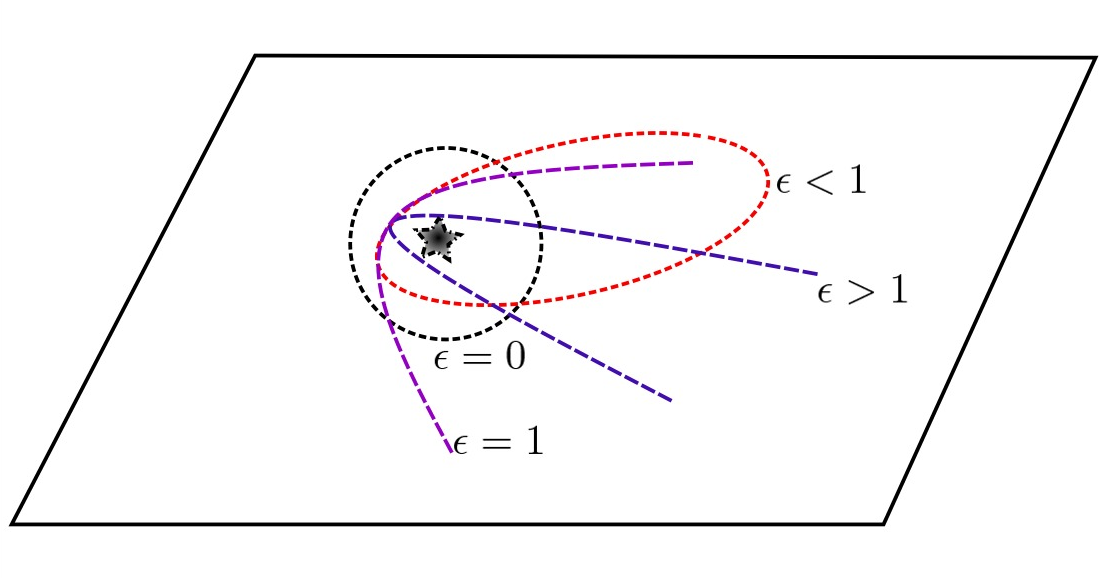
\includegraphics[width=9cm]{figura14.png} 
	\caption{ Trayectorias según el valor de $\epsilon$.}
	\label{fig.1}
	\end{center}
\end{figure}


En todos los casos por comodidad, para ubicar en forma apropiada el eje polar consideraremos $\alpha=0$



\begin{table}[htbp]
\begin{center}
\begin{tabular}{|l|l|l|}
\hline
$\epsilon$& Orbita & Energia\\
\hline \hline
$\epsilon > 1$ & Hiperbola & $E>0$ \\ \hline
$\epsilon = 1$ & Parabola & $E=0$ \\ \hline
$\epsilon < 1$ & Elipse & $E<0$ \\ \hline
$\epsilon=0$   & Circunferencia & $E= \displaystyle -\frac{mk^2}{2L_0^2}$ \\ \hline
\end{tabular}
\caption{Tabla muy sencilla.}
\label{tabla:sencilla}
\end{center}
\end{table}












\section{Problema Unidimensional Equivalente}


Recordemos de que la energía asociada a un movimiento central se conserva y esta dada por 

\begin{equation}
E= \frac{1}{2}m\dot{r}^2 + \frac{L_0^2}{2mr^2} -\frac{k}{r}
\end{equation}

pero, dado que  $V_{ef} = \displaystyle \frac{L_0^2}{2mr^2} -\frac{k}{r} $, obtenemos

\begin{equation}
E=\frac{1}{2}m\dot{r}^2 + V_{ef}
\end{equation}

Analizando con fuerza esta ultima ecuación, notemos que es una expresión análoga al caso unidimensional  cuando $\vec{F}$ depende de una variable, es decir, podemos discutir la ecuación () usando los mismos métodos con los cuales hemos estudiado el movimiento unidimensional conservativo. \\

Sea $U(r)= - \displaystyle \frac{k}{r}$, luego el potencial efectivo tendrá la forma indicada por la figura (\ref{fig35})


\begin{figure}[H]
	\begin{center}
	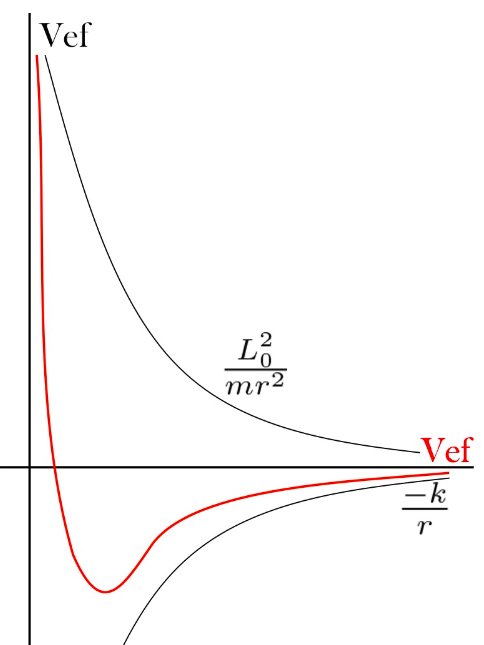
\includegraphics[width=6cm]{figura151.png} 
	\caption{ Potencial Efectivo.}
	\label{fig35}
	\end{center}
\end{figure}


 A partir de este gráfico es posible obtener una descripción cualitativa de los posibles movimientos.

Se tiene que $E= T + V_{ef}$, donde $T \geq 0$. El movimiento no es posible si $T<0$, por tanto, una region para la cual $T<0$ define una region prohibida para el movimiento de una particula \\

 
En este potencial, los cuerpos con energía negativa quedaran "ligados"\ con el potencial y su movimiento estará acotado por dos radios finitos $r_1$ y $r_2$. Mientras que, para las energías positivas, el cuerpo puede alejarse indefinidamente del origen. Para analizar estas ideas con mas detalle consideremos los siguientes casos indicados en la figura (3.7). 




\textbf{\underline{Caso $E_1>0$ :}} \\

La partícula viene desde el infinito y alcanza un radio mínimo llamado \textit{punto de retorno}.

\begin{equation}
E_1 - V_{ef}= \frac{1}{2} m \dot{r}^2  
\end{equation}


si $r=r_1$  tenemos $E=V_{ef}$, luego cuando $E_1 > V_{ef}$ se tiene $r_1<r<\infty$. \\

Notemos que la partícula no podrá estar a una distancia menor que $r_1$ , ya que, si esto ocurre $E_1<V_{ef} \Rightarrow \displaystyle \frac{1}{2}m\dot{r}^2<0$.  \\
\\
\underline{Observación}: Notemos que el valor de $r$ no tiene limite superior, lo que implica que la órbita no es cerrada. \\
\\

\textbf{\underline{Caso $E_2=0$} :} \\

La particula viene desde el infinito y alcanza su punto de retorno  en $r_2=\displaystyle\frac{L_0}{2mk}$ \\
\\


\textbf{\underline{Caso $E_3 < 0$ :}} \\

En este caso el movimiento esta limitado por dos puntos de retorno $r_3$ y $r_3 '$

\begin{equation}
r_3' < r < r_3 
\end{equation}  

\textbf{\underline{Observaciones}:}

\begin{itemize}
\item El movimiento esta limitado a una región del espacio.
\item El movimiento no necesariamente es cerrado.
\end{itemize}


\begin{figure}[H]
	\begin{center}
	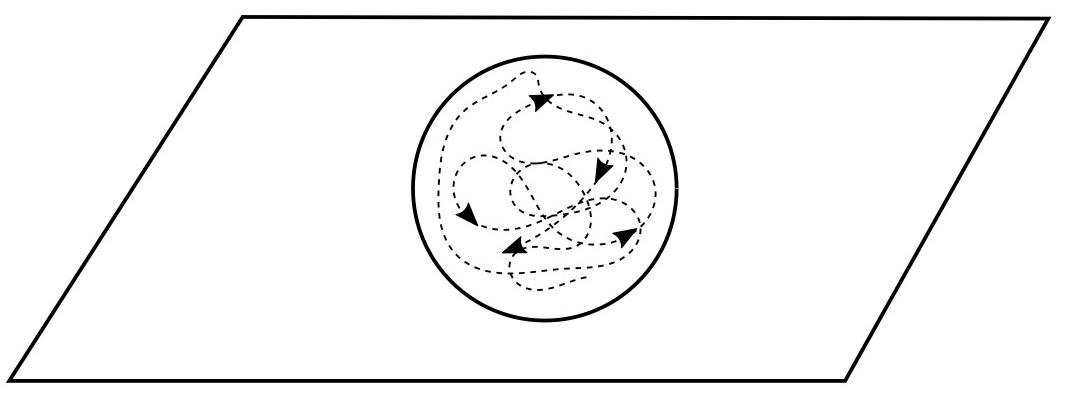
\includegraphics[width=11cm]{figura17.png} 
	\caption{ Representación de un pozo potencial}
	\label{fig36}
	\end{center}
\end{figure}

Se dice que este movimiento esta confinado en un \textit{pozo potencial}. \\
\\

\textbf{\underline{Caso $E_4$ :}} Este caso Corresponde a la energía mínima, en el cual podemos ver que  el radio del movimiento no varia entre un máximo y un mínimo. Esto ocurre cuando $E=V_{ef}$, luego

\begin{equation}
E-V_{ef}=\frac{1}{2} m \dot{r}^2 = 0 \\
\Rightarrow \dot{r}=0 \\
\Rightarrow r=cte
\end{equation}

Por tanto, la órbita es una circunferencia.


\begin{figure}[H]
	\begin{center}
	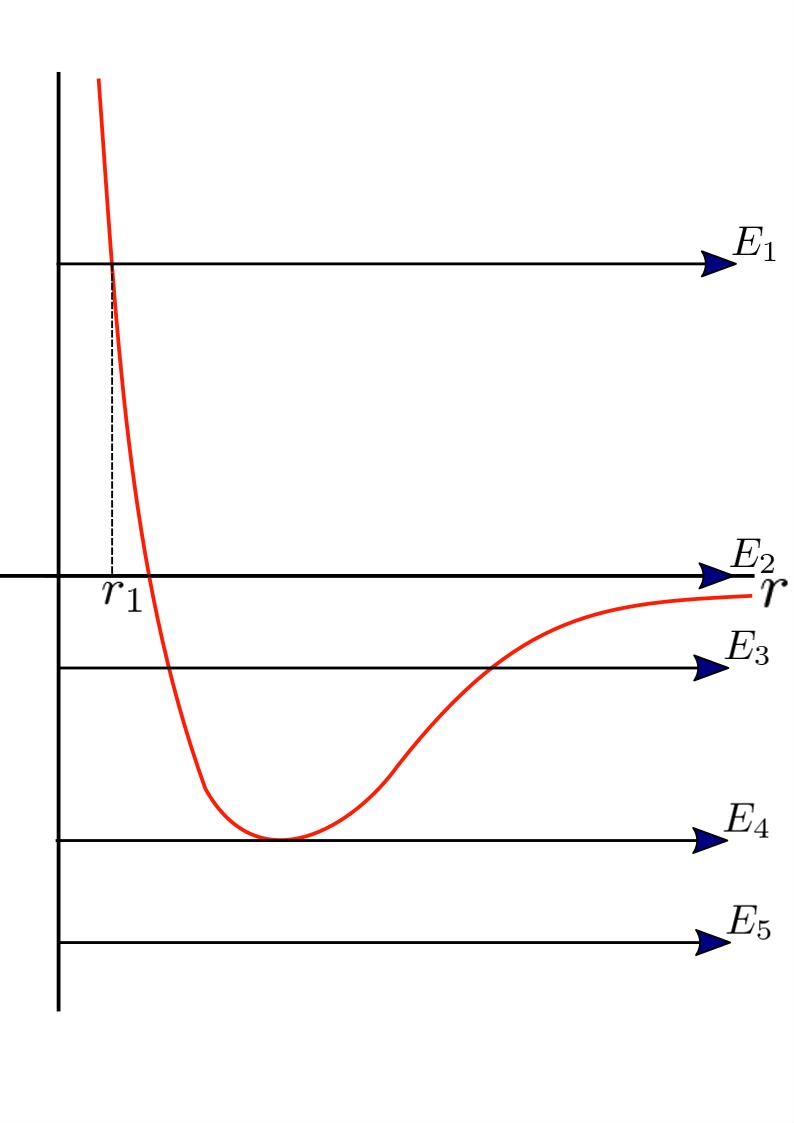
\includegraphics[width=6cm]{figura16.jpeg} 
	\caption{ Casos posibles para E.}
	\label{fig.1}
	\end{center}
\end{figure}














































\chapter{Grados de Libertad, Vinculos y Coordenadas Generalizadas}


\textbf{\textit{Definición:}} el \textit{grado de libertad} que posee un cuerpo o sistema es el numero total de posibles movimientos linealmente independientes que tiene y se denota con la letra $f$. \\
\\


\textbf{Ejemplo 1:} Particula puntual \\

La partícula puntual esta descrita por tres coordenadas linealmente independientes. Por tanto $f=3$ \\


\begin{figure}[H]
	\begin{center}
	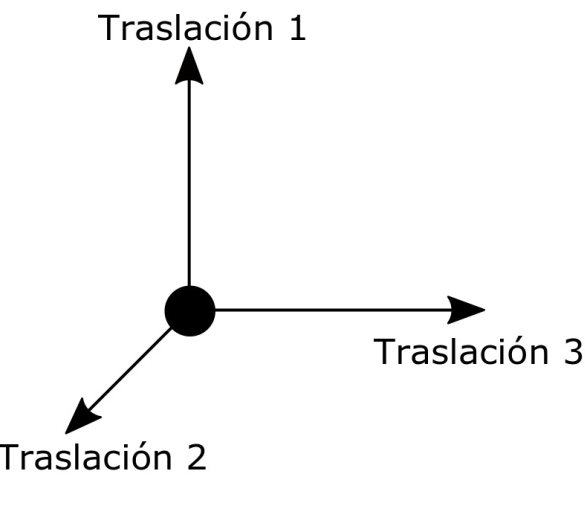
\includegraphics[width=8cm]{figura18.png} 
	\caption{ Grados de libertad de una partícula puntual.}
	\label{fig.1}
	\end{center}
\end{figure}

\textbf{Ejemplo 2:} Una papa 
\\

Una papa posee seis movimientos linealmente independientes.
 
\begin{figure}[H]
	\begin{center}
	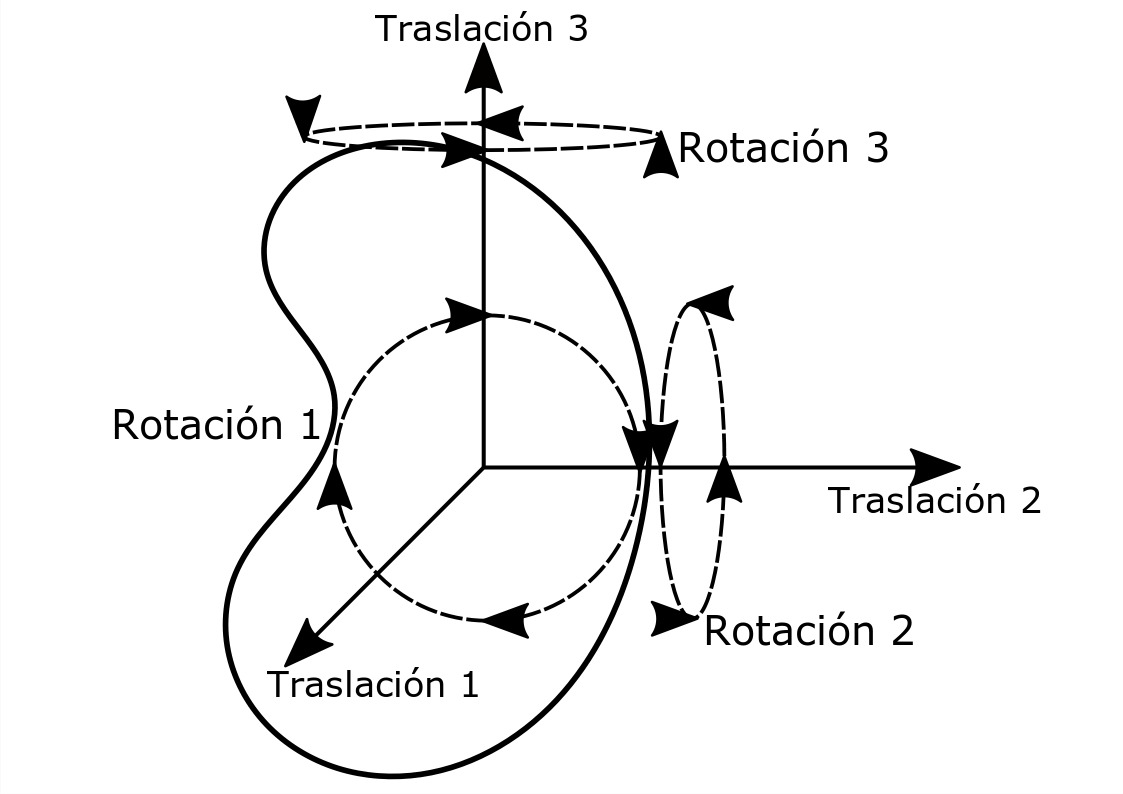
\includegraphics[width=9cm]{figura19.jpeg} 
	\caption{ Grados de libertad de una papa.}
	\label{fig.1}
	\end{center}
\end{figure}

 Luego f=6. \\   

Sin embargo existen casos en los cuales el sistema esta sometido a fuerzas provenientes de \textit{vínculos}, entonces en ese caso decimos que el sistema se encuentra ligado o vinculado.









\section{Vinculos}


\textbf{\textit{Definición:}} Un vinculo es una restricción al movimiento que se expresa en una relación matemática entre las coordenadas independientes a las leyes de newton \\
\\


\textbf{Ejemplo 1:} Una cuenta de ábaco es un sistema vinculado por el alambre el cual restringe su movimiento. \\
\\

\textbf{Ejemplo 2:} Partícula de masa $m$ girando alrededor de un punto mediante a una cuerda. 

\begin{figure}[h]
	\begin{center}
	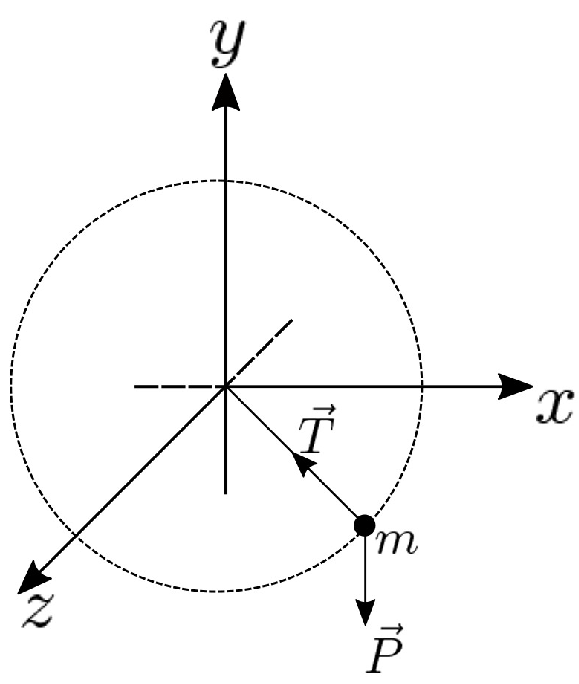
\includegraphics[width=7cm]{figura20.png} 
	\caption{ Trayectoria de la partícula (Ejemplo 2).}
	\label{fig.1}
	\end{center}
\end{figure}


Aplicando la segunda ley de Newton 
\begin{equation}
m\vec{a}=\vec{T}+\vec{P}
\end{equation}

Considerando que 

\begin{eqnarray}
\vec{T}=-T\sin{\phi} \ \hat{\imath}+T\cos{\phi} \ \hat{\jmath}
\end{eqnarray}

podemos expresar $(4.1)$ como

\begin{equation}
m \left( \ddot{x} \hat{\imath} + \ddot{y} \hat{\jmath} \right) = \underbrace{-T\sin{\phi}}_{T_x} \ \hat{\imath} + \left( \underbrace{T\cos{\phi}}_{T_y} - mg \right) \hat{\jmath}
\end{equation} 


luego, las ecuaciones del movimiento están dadas por

\begin{eqnarray}
m\ddot{x}&=&T_x \\
m\ddot{y}&=&T_y - mg
\end{eqnarray}

pero existe una ligadura asociada a este sistema, la cual esta dada por la relación

\begin{equation}
x^2 + y^2 = L^2
\end{equation}

de la ecuacion anterior podemos ver una relacion entre $x$ e $y$  dada por

\begin{equation}
y=\sqrt{L^2 - x^2}
\end{equation}


Reemplazando (4.7) en (4.52) obtenemos

\begin{eqnarray}
m\ddot{x}&=&T_x \\
m\left( \frac{-x \ddot{x}-\dot{x}^2}{\sqrt{L^2 - x^2}}- \frac{x^2 \dot{x}^2}{\left(L^2 - x^2\right)^{\frac{3}{2}}} \right)&=& T_x - mg
\end{eqnarray}

Por tanto,  $f=1$




\section{Clasificación de los Vínculos}

\subsection{Vínculos Holonomos y Anholonomos}


Un vinculo se considera \textit{holonomo} cuando es posible expresar la condición de ligadura mediante una relación entre las posiciones de las partículas 	y el tiempo de la forma:

\begin{equation}
f(x_1 , x_2 , x_3 , ..., x_n, t)
\end{equation}

A su vez, los enlaces \textit{holonomos} se denominan \textit{escleronomos} si no dependen del tiempo, y \textit{reónomos} en caso contrario. \\

Los enlaces \textit{anholónomos} son en general todos aquellos que no son \textit{holonomos}, no pudiendo expresarse mediante ecuaciones del tipo (4.10)\\ \\


\textbf{Ejemplo:} Consideremos un sistema de $N$ partículas sometido a $n$ vínculos holonomos, es decir

\begin{eqnarray} \nonumber
f_1(\vec{x}_1, \vec{x}_2, \vec{x}_3, ..., \vec{x}_N )&=&0 \\ \nonumber
f_2(\vec{x}_1, \vec{x}_2, \vec{x}_3, ..., \vec{x}_N )&=&0 \\ \nonumber
f_3(\vec{x}_1, \vec{x}_2, \vec{x}_3, ..., \vec{x}_N )&=&0 \\ \nonumber
&\vdots& \\ \nonumber
f_n(\vec{x}_1, \vec{x}_2, \vec{x}_3, ..., \vec{x}_N ) &=& 0 
\end{eqnarray}


En este caso tenemos $n$ vínculos holonomos, expresados  mediante n ecuaciones que pueden ser usadas para eliminar $n$ de las $3N$ coordenadas. Luego, nos quedan $3N-n$ coordenadas independientes. Por tanto el sistema tiene $f=3N-n$ grados de libertad. \\ \\

\textbf{\underline{Nota}:} En este apunte usaremos solo vínculos holonomos, a menos que se indique lo contrario.














\section{Reacciones Vinculares}


Consideremos la figura (\ref{fig44}). 
Las tres superficies de la figura son vínculos, pues restringen el movimiento, y cada una de estas genera una fuerza que actuá sobre el cuerpo, estas fuerzas se llaman \textit{reacciones vinculares}. \\

\begin{figure}[h]
	\begin{center}
	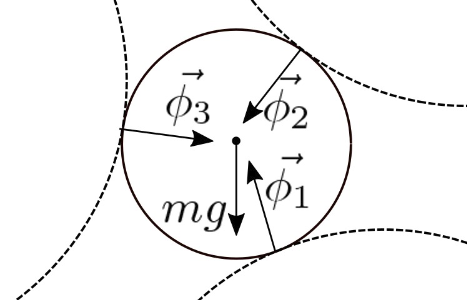
\includegraphics[width=7cm]{figura211.png} 
	\caption{ Reacciones vinculares.}
	\label{fig44}
	\end{center}
\end{figure}


\textbf{\underline{Observación 1}:} Usaremos la letra griega $\phi$ para indicar reacciones vinculares. \\ 

\textbf{\underline{Observación 2}:}  Debido a la presencia de los vínculos asociados a un sistema, las ecuaciones de movimiento

\begin{equation}
\sum_{i} m \vec{a}_i = \sum_{i} F_{ext \rightarrow i} + \sum_{i} \vec{\phi}_{\alpha} 
\end{equation}

no son todas independientes. \\ \\


\textbf{Hipotesis:} La reaación vincular $\phi_\alpha$ es siempre  perpendicular a la superficie de contacto $f_\alpha$. Es decir

\begin{eqnarray}
\phi_{\alpha} \parallel \sum_{i=1}^N \nabla_i f_{\alpha} \\
\Rightarrow \phi_{\alpha}=\lambda_{\alpha} \sum_{i=1}^N \nabla_i f_{\alpha}
\end{eqnarray}


luego (4.11) toma la forma

\begin{equation}
\sum_{i=1}^N m \vec{a}_i = \sum_{i=1}^N \vec{F}_{ext \rightarrow i} + \sum_{\alpha=1}^{N} \lambda_{\alpha} \sum_{i=1}^N \nabla_i f_{\alpha}
\end{equation}




\textbf{Ejemplo:} Péndulo simple \\ 

la tensión de un péndulo es perpendicular a la superficie esférica en la que puede moverse la partícula, es decir, va en la dirección radial, a lo largo de la varilla. En una superficie lisa como la de una mesa pulida, es normal a la superficie de la mesa.

\begin{figure}[H]
	\begin{center}
	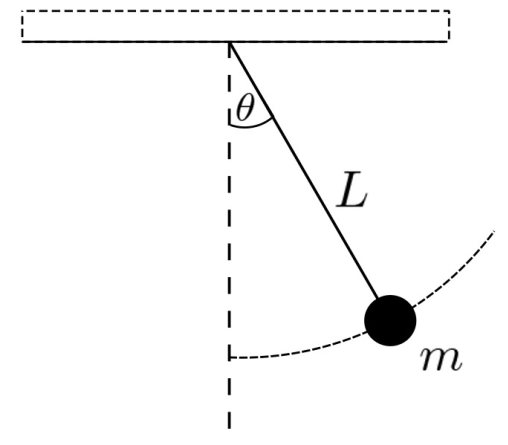
\includegraphics[width=6cm]{figura22.png} 
	\caption{ Péndulo simple.}
	\label{fig.1}
	\end{center}
\end{figure}


\textbf{\underline{Observación}:} Consideremos un bloque en un plano inclinado con roce 

\begin{figure}[H]
	\begin{center}
	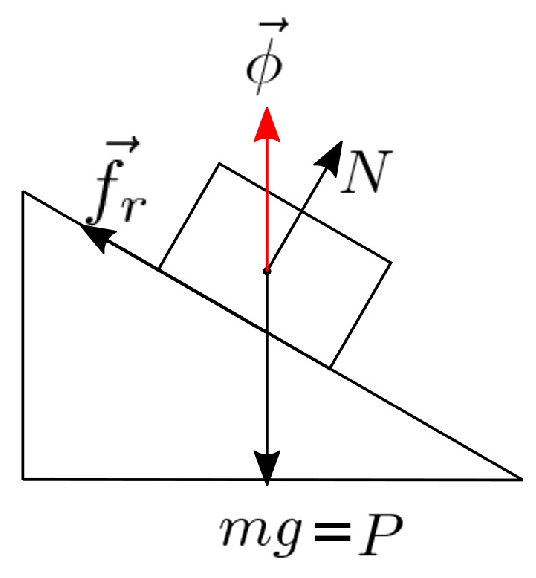
\includegraphics[width=6cm]{figura23.png} 
	\caption{ Diagrama del plano inclinado.}
	\label{fig.1}
	\end{center}
\end{figure}

Cuando el roce esta presente, la reacción vincular ya no es perpendicular a la superficie vincular

\begin{equation}
\vec{\phi} = \vec{f}_r + \vec{N}.
\end{equation}

Frente a este tipo de casos se debe introducir una nueva nomenclatura, llamaremos \textit{fuerzas activas} a aquellas que no son reacciones vinculares. Luego, la fuerza de roce es considerada una fuerza activa, mientras que la normal sigue siendo una reacción vincular.





\section{Coordenadas Generalizadas}

La dificultad que introducen los vínculos, debido a que no todas las coordenadas son independientes, puede solucionarse por medio de la introducción de coordenadas generalizadas. \\

Consideremos un sistema con $i=1,2,..., N$ partículas, el cual esta sometido a $k=1,2,..., n$ vínculos holonomos expresados mediante $k=1,2,...,n$ ecuaciones de la forma $f^k(\vec{x}_i)$. La eliminación de las coordenadas dependientes se puede hacer introduciendo  $3N-n$ coordenadas independientes

\begin{equation}
\left\{ q^a \right\}_{a=1}^{3N-n}
\end{equation}

Esto involucra una transformación de coordenadas 


\begin{equation}
\vec{x}_i = \vec{x_i}(q^a) 
\end{equation}

es decir 


\begin{eqnarray}
\vec{x}_1 &=&\vec{x}_1 \left( q^1 , q^2 , ... , q^{3N-n} \right)  \\
\vec{x}_2 &=&\vec{x}_2 \left( q^1 , q^2 , ... , q^{3N-n} \right) \\
&\vdots& \\
\vec{x}_N &=&\vec{x}_N \left( q^1 , q^2 , ... , q^{3N-n} \right) 
\end{eqnarray}

tal que


\begin{equation}
f_{\alpha}\left( x_i(q^a) \right) \equiv 0.
\end{equation} 
\\



El espacio de dimensión $3N-n$ formado por todos los posibles conjuntos de coordenadas generalizadas se define como el \textit{espacio de configuraciones}. La evolución del sistema a través del tiempo estará representada por una curva en el espacio de configuraciones (figura \ref{fig47}).  \\

\begin{figure}
	\begin{center}
	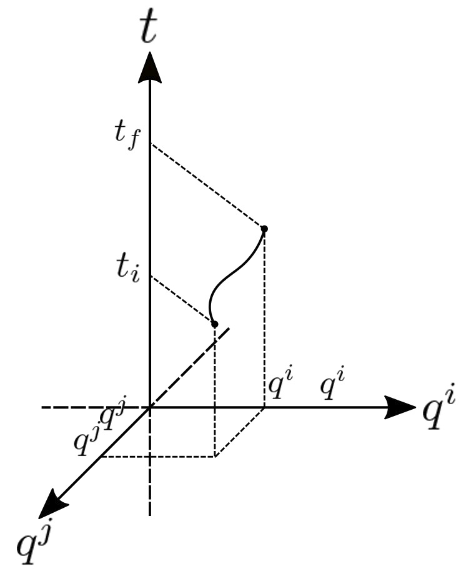
\includegraphics[width=7cm]{figura2411.png} 
	\caption{ Espacio de configuraciones.}
	\label{fig47}
	\end{center}
\end{figure}



\textbf{Ejemplo}: Pendulo simple \\ 

En este caso tenemos una particula ligada a un plano y una cuerda, por tanto el sistema tiene $f=1$ grado de libertad, esto indica que hay una coordenada generalizada. La transformacion de coordenadas esta dada por

\begin{eqnarray}
x=L \cos{\theta} \\
y=L \sin{\theta}
\end{eqnarray}

donde $\theta$ es la coordenada generalizada que conforma el espacio de configuraciones del sistema. 

\begin{figure}[H]
	\begin{center}
	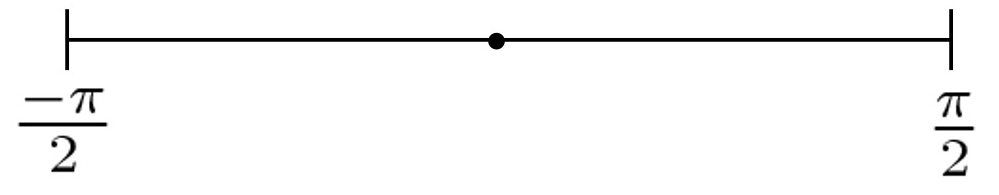
\includegraphics[width=8cm]{figura241.png} 
	\caption{ Espacio de configuración de un pendulo simple.}
	\label{fig.1}
	\end{center}
\end{figure}


\textbf{\underline{Observación}:} No existe necesariamente relación entre el espacio de configuraciones y el espacio físico tridimensional.









\subsection{Fuerza Generalizada}	


Consideremos un diferencial de $f_\alpha(\vec{x_i})$ como esta indicado  en la figura () 


\begin{figure}[h]
 \centering
  \subfloat[Representación de $f_{\alpha}$]{
   \label{fig49}
    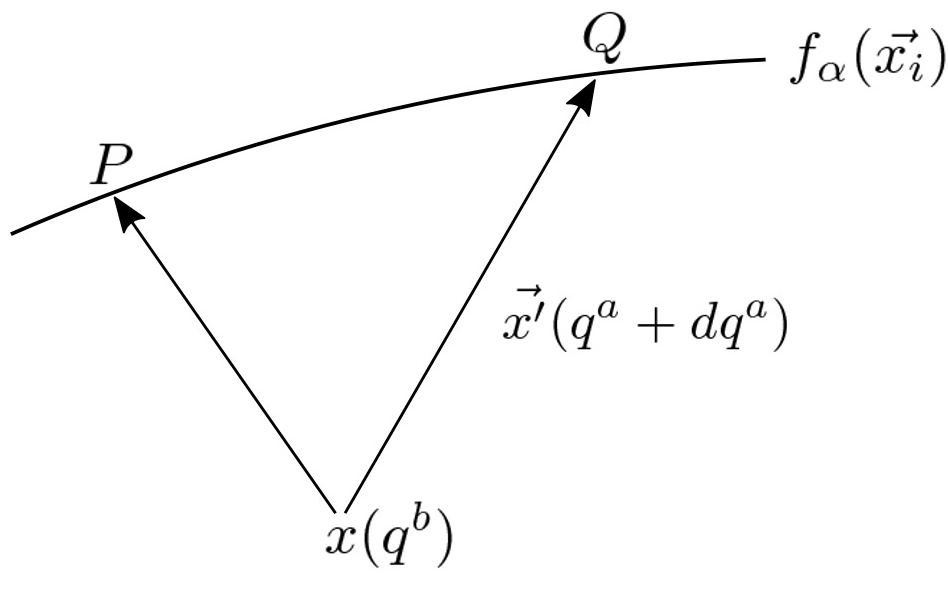
\includegraphics[width=0.5\textwidth]{figura25.png}}
  \subfloat[Relación entre $\nabla f$ y $\displaystyle \frac{\partial \vec{x}}{\partial q^a}$ ]{
   \label{fig491}
    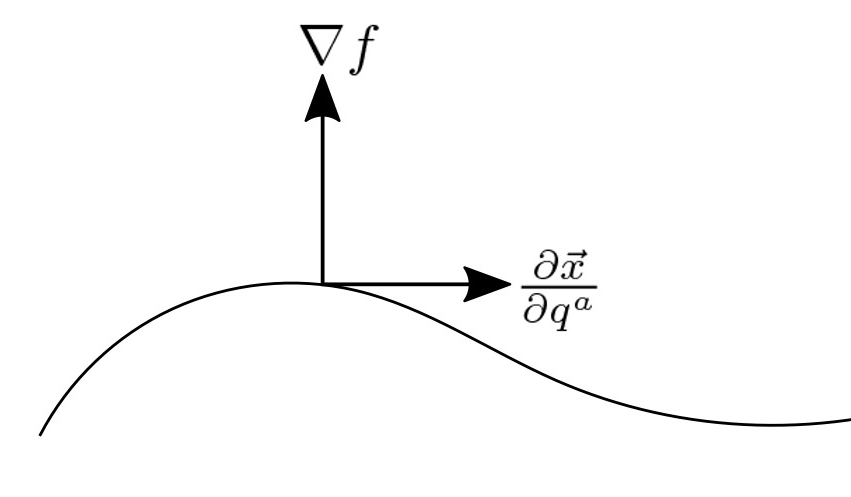
\includegraphics[width=0.5\textwidth]{figura26.png}}
 \label{f:animales}
\end{figure}

notemos que 

\begin{eqnarray}
df_{\alpha}&=&f_{\alpha}\left(\vec{x_i}\left(q^a+dq^a\right)\right)-f_{\alpha}(\vec{x}_i(q^a)) \\
&=& \sum_{i=1}^N \vec{\nabla}_{i} f_{\alpha} \frac{\partial \vec{x}_i }{\partial q^a}=0 \\
&&\Rightarrow \sum_{i=1}^N \vec{\nabla}_{i} f_{\alpha} \frac{\partial{\vec{x}_i}}{{\partial q^a}} = 0
\end{eqnarray}


Por tanto,  $\displaystyle\frac{\partial \vec{x}_i}{\partial q^a} \perp \vec{\nabla}_{i} f_{\alpha}$ \\

Por otra parte, retomemos la expresión (4.14)

\begin{equation}
\sum_{i=1}^N m\vec{a}_i = \sum_{i=1}^N \vec{F}_{ext \rightarrow i} + \sum_{\alpha=1}^N \lambda_{\alpha} \sum_{i=1}^N \vec{\nabla_{i}} f_{\alpha} 
\end{equation}

multiplicando la ecuación anterior por $\displaystyle \frac{\partial \vec{x}_i}{\partial q^a}$ obtenemos

\begin{eqnarray}
\sum_{i=1}^N m\vec{a}_i \frac{\partial \vec{x}_i}{\partial q^a} &=& \sum_{i=1}^N F_{ext \rightarrow i}\frac{\partial \vec{x}_i}{\partial q^a} + \sum_{\alpha=1}^N \lambda_{\alpha} \sum_{i=1}^N \cancelto{0}{\vec{\nabla_{i}} f_{\alpha} \frac{\partial \vec{x}_i}{\partial q^a}} \\
\sum_{i=1}^N m \vec{a}_i \frac{\partial \vec{x}_i}{\partial q^a} &=& \sum_{i=1}^N F_{ext \rightarrow i} \frac{\partial \vec{x}_i}{\partial q^a}
\end{eqnarray}

donde, la expresión $\displaystyle Q_a= \sum_{i=1}^N F_{ext \rightarrow i} \frac{\partial \vec{x}_i}{\partial q^a}$ es la \textit{fuerza generalizada} correspondiente a la coordenada generalizada $q^a$. Finalemnte,

\begin{equation}
Q_a =  \sum_{i=1}^N F_{ext \rightarrow i} \frac{\partial \vec{x}_i}{\partial q^a}.
\end{equation}

Esta ultima expresión tomara relevancia al momento de estudiar las ecuaciones de Euler-lagrange en el capitulo $6$






























\chapter{Principio de los Trabajos Virtuales}


\section{Desplazamiento Virtual}


Un \textit{desplazamiento virtual} es un movimiento puramente geométrico e imaginario consistente con las fuerzas y las ligaduras del sistema físico presentes en $t=t_0$. 


\begin{figure}[H]
	\begin{center}
	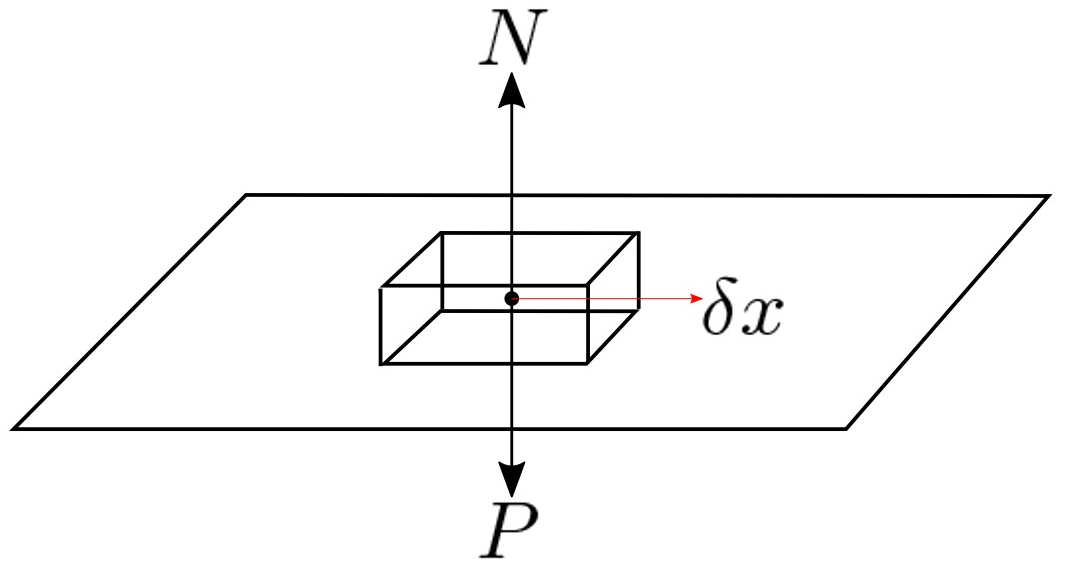
\includegraphics[width=8cm]{figura27.png} 
	\caption{ Desplazamiento virtual sobre un plano.}
	\label{fig.1}
	\end{center}
\end{figure}

Notación:

\begin{eqnarray}
d\vec{x} &:& \textrm{Desplazamiento fisico} \\
d\vec{\delta} &:& \textrm{Desplazamiento virtual}
\end{eqnarray}



\section{Trabajo Virtual}

El trabajo virtual $\delta W$ realizado por una fuerza $\vec{F}$ en un desplazamiento virtual $\delta \vec{x}$ se define como


\begin{equation}
\delta W=\vec{F} \cdot \delta\vec{x}
\end{equation}


\textbf{Ejemplo:} Consideremos una partícula libre en reposo sometida a fuerzas externas. Luego

\begin{equation}
\delta W = \sum_{i} \vec{F}_i \cdot \delta\vec{x}=0
\end{equation}


El trabajo virtual ejercido por las fuerzas externas sobre una partícula libre en equilibrio es cero, independiente  de cual sea el el desplazamiento virtual de la partícula. 









\section{Teorema de Torricelli}


Supongamos que todas las fuerzas activas son conservativas, es decir

\begin{equation}
\vec{F}= -\vec{\nabla} U
\end{equation}

Usando el principio de los trabajos virtuales

\begin{eqnarray}
\delta W = \vec{F} \cdot \delta\vec{x}= -\vec{\nabla} U \cdot \delta\vec{x}=-\delta U
\end{eqnarray}

por otra parte, $\displaystyle \delta W = \sum_{i} \vec{F}_i \cdot \delta \vec{x}_i$ es nulo para los desplazamientos virtuales. Por tanto, el principio de los trabajos virtuales para el caso donde $\vec{F}$ es una fuerza conservativa se puede expresar de la forma:

\begin{equation}
\delta U = 0
\end{equation}

\textbf{\textit{Teorema:}} La energía potencial de un sistema que esta en equilibrio asume un valor extremo. \\ \\


\textbf{Casos} : \\ 

\textbf{\underline{Equilibrio estable}:} La partícula retorna a su punto de equilibrio. 

\begin{figure}[H]
	\begin{center}
	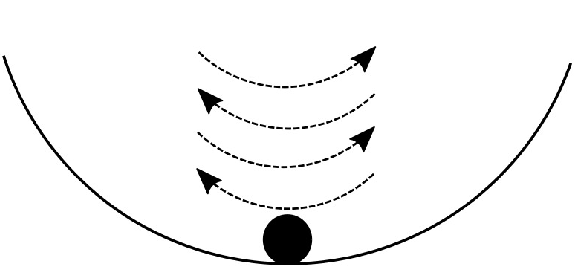
\includegraphics[width=8cm]{figura28.png} 
	\caption{ Equilibrio estable.}
	\label{fig.1}
	\end{center}
\end{figure}

\textbf{\underline{Equilibrio inestable}:} La partícula no retorna a su posición de equilibrio.

\begin{figure}[H]
	\begin{center}
	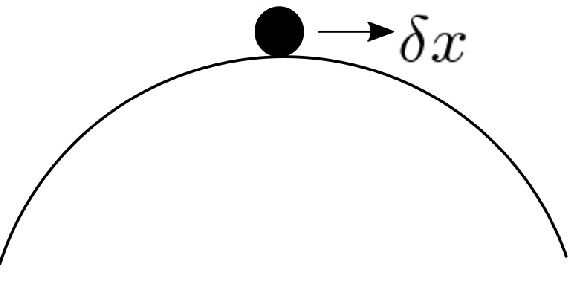
\includegraphics[width=8cm]{figura29.png} 
	\caption{Equilibrio inestable.}
	\label{fig.1}
	\end{center}
\end{figure}

\textbf{\underline{Equilibrio indiferente}:} La partícula permanece en equilibrio en su posición.


\begin{figure}[H]
	\begin{center}
	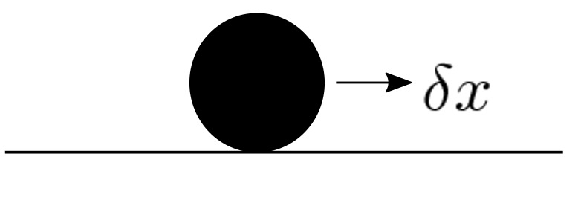
\includegraphics[width=8cm]{figura30.png} 
	\caption{ Equilibrio indiferente.}
	\label{fig.1}
	\end{center}
\end{figure} 






















\section{Principio de D’Alembert}


Consideremos un sistema de $N$ partículas sometidas a fuerzas externas, dicho sistema es descrito por la segunda ley de Newton.

\begin{equation}
m \ddot{x}_i = \vec{F}_{ext \rightarrow i}
\end{equation}

Una pregunta interesante que podemos formular es : ¿ Es posible aplicar el principio de los trabajos virtuales a un sistema como este el cual no se encuentra en equilibrio? \\	


La respuesta es si, y es suministrada por el \textit{principio de D’Alembert}, el cual reduce el problema dinámico  a un problema estático  mediante la definición de \textit{fuerzas inerciales} $\vec{\varphi}_i$

\begin{equation}
\vec{\varphi}= -m_i\ddot{x}_i
\end{equation}


Luego,

\begin{equation}
\vec{F}_{ext \rightarrow i} + \vec{\varphi}_i =0
\end{equation}

Aplicamos el principio de los trabajos virtuales:

\begin{equation}
\delta W=\sum_{i=1}^N \left( F_{ext \rightarrow i} + \vec{\varphi}_i  \right) \cdot \delta \vec{x}_i
\end{equation}

En el caso donde existan vínculos holonomos (compatibles con el desplazamiento virtual), la relación se modifica debido a la presencia de reacciones vinculares asociadas al sistema. Luego, la ecuación general resulta:

\begin{equation}
\vec{F}_{ext \rightarrow i} + \vec{\varphi}_i + \vec{\phi}_i =0
\end{equation} 


Entonces:


\begin{equation}
\delta W=\sum_{i=1}^N \left( F_{ext \rightarrow i} + \vec{\varphi}_i  + \vec{\phi}_i \right) \cdot \delta \vec{x}_i = 0
\end{equation}

Dado que el desplazamiento virtual es compatible con los vínculos, se tiene :

\begin{equation}
\phi_i \cdot \delta \vec{x}_i = 0 \ \ \forall i
\end{equation}


Por tanto, el principio de D’Alembert puede escribirse como 

\begin{equation}
\sum_{i=1}^N \left( F_{ext \rightarrow i} - m \ddot{\vec{x}}_i \right) \cdot \delta \vec{x}_i = 0.
\end{equation}

































\chapter{Formalismo Lagrangiano} 


\section{Ecuaciones de Euler-Lagrange}

Consideremos un sistema de $N$ partículas en movimiento descrito por (4.30). A partir de esta expresión hemos definido la fuerza generalizada como


\begin{equation}
Q_a = m \vec{a}_i \frac{\partial \vec{x}_i}{\partial q^a}.
\end{equation}

Es de nuestro interés expresar $Q_a$ en función de las coordenadas generalizadas 



\begin{eqnarray}
Q_a &=& m \vec{a}_i \frac{\partial \vec{x}_i}{\partial q^a} = m \frac{d\vec{v}_i}{dt} \frac{\partial \vec{x}_i}{\partial q^a} = \frac{d}{dt} \left( m \vec{v}_i \right) \frac{\partial \vec{x}_i}{\partial q^a} \\
&=&\frac{d}{dt} \left( m\vec{v}_i \frac{\partial \vec{x}_i}{\partial q^a}   \right) - m\vec{v}_i \frac{d}{dt} \left( \frac{\partial \vec{x}_i}{\partial q^a} \right)
\end{eqnarray}

Por otra parte, notemos que $\displaystyle \frac{\partial \vec{v}_i}{\partial \dot{q}^a} = \frac{\partial \vec{x}_i}{\partial q^a}$, en efecto



\begin{eqnarray}
\frac{\partial \vec{v}_i}{\partial \dot{q}^a} &=& \frac{\partial}{\partial \dot{q}^a} \left( \frac{\partial \vec{x}_i}{\partial q^b} \dot{q}^b \right) \\
&=& \cancelto{0 }{\frac{\partial}{\partial \dot{q}^a} \left( \frac{\partial \vec{x}_i}{\partial q^b}  \right)} \dot{q}^b + \frac{\partial \vec{x}_i}{\partial q^b} \frac{\partial \dot{q}^b}{\partial \dot{q}^a} \\
&=&\frac{\partial \vec{x}_i}{\partial q^b} \delta^b_{a} \\
&=& \frac{\partial \vec{x}_i}{\partial q^a}
\end{eqnarray} 

Reemplazando esta ultima expresión en (6.3) obtenemos:

\begin{eqnarray}
Q_a&=&\frac{d}{dt} \left( m\vec{v}_i \frac{\partial \vec{v}_i}{\partial \dot{q}^a}   \right) - m\vec{v}_i \frac{d}{dt} \left( \frac{\partial \vec{x}_i}{\partial q^a} \right) \\
&=& \frac{d}{dt} \left[ \frac{\partial}{\partial q^a} \left(\frac{1}{2} m\vec{v}_i \vec{v}_i \right)  \right] - m\vec{v}_i \frac{d}{dt} \left( \frac{\partial \vec{x}_i}{\partial q^a} \right)
\end{eqnarray}


Se define la \textbf{\textit{energía cinética}} del sistema como:

\begin{equation}
T(q,\dot{q}) = \frac{1}{2}m\vec{v}_i \vec{v}_i 
\end{equation}

Entonces (6.9) toma la forma:

\begin{eqnarray}
Q_a = \frac{d}{dt} \left( \frac{\partial T}{\partial \dot{q}^a} \right) -  m\vec{v}_i \underbrace{\frac{d}{dt} \left( \frac{\partial \vec{x}_i}{\partial q^a} \right)}_{(*)}
\end{eqnarray}

de la expresión (*) vemos que:

\begin{eqnarray}
\frac{d}{dt} \left( \frac{\partial \vec{x}_i}{\partial q^a} \right) &=& \frac{\partial}{\partial q^b} \left( \frac{\partial \vec{x}_i}{\partial q^a} \right) \dot{q}^b \\
&=& \frac{\partial}{\partial q^a} \left( \frac{\partial \vec{x}_i}{\partial q^b} \right) \dot{q}^b \\
&=&\frac{\partial}{ \partial q^a} \left( \frac{d\vec{x}_i}{dt} \right) \\
&=&\frac{\partial \vec{v}_i}{\partial q^a}
\end{eqnarray}


Reemplazando (6.15) en (6.11) obtenemos

\begin{eqnarray}
Q_a &=& \frac{d}{dt} \left( \frac{\partial T}{\partial \dot{q}^a} \right) -  m\vec{v}_i \frac{\partial \vec{v}_i}{\partial q^a} \\
&=& \frac{d}{dt} \left( \frac{\partial T}{\partial \dot{q}^a} \right) - \frac{\partial}{\partial q^a} \left(\frac{1}{2} m\vec{v}_i \vec{v}_i \right) \\
&=&\frac{d}{dt} \left( \frac{\partial T}{\partial \dot{q}^a} \right) - \frac{\partial T}{\partial q^a} 
\end{eqnarray}

Por tanto


\begin{equation}
Q_a=\frac{d}{dt} \left( \frac{\partial T}{\partial \dot{q}^a} \right) - \frac{\partial T}{\partial q^a}  \ \ \ \ \ \ a=1,2,...,f=3N-n
\end{equation}

Estas son las \textit{ecuaciones de Lagrange de segunda especie} \\ \\

\textbf{Ejemplo:} Péndulo simple  \\


\begin{figure}
	\begin{center}
	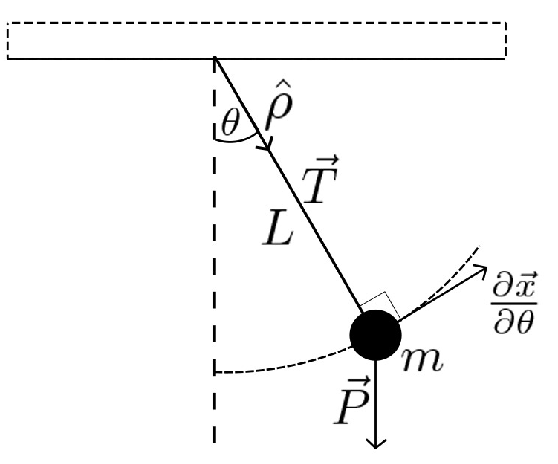
\includegraphics[width=8cm]{figura31.png} 
	\caption{ Pendulo simple.}
	\label{fig.1}
	\end{center}
\end{figure} 


En este caso tenemos una coordenadas generalizada $q^1=\theta$, luego 

\begin{eqnarray}
\vec{x}&=& L \sin{\theta} \ \hat{\imath} - L\cos{\theta} \ \hat{\jmath} \\
&\Rightarrow& \frac{d \vec{x}}{d\theta} = L \cos{\theta} \ \hat{\imath} + L\sin{\theta} \ \hat{\jmath} = L \hat{\phi}
\end{eqnarray}

la fuerza generalizada esta dada por


\begin{eqnarray}
Q&=&(\vec{P}+\vec{T}) \cdot L\hat{\phi} 
= L\vec{P} \cdot \hat{\phi} + L \cancelto{0}{\vec{T} \cdot \hat{\phi}} \\
Q&=&-Lmg \ \hat{\jmath} \cdot \hat{\phi} = -Lmg \ \hat{\jmath} \left( \cos{\theta} \ \hat{\imath} + \sin{\theta} \ \hat{\jmath} \right) \\
Q&=&-mgL \sin{\theta}
\end{eqnarray}


Por otra parte la energía cinética es:

\begin{eqnarray}
T=\frac{1}{2} m L^2 \dot{\theta}^2
\end{eqnarray}

Finalmente, la ecuación de movimiento resulta 

\begin{eqnarray}
\frac{d}{dt} \left[ \frac{\partial}{\partial \theta} \left( \frac{1}{2} mL^2 \dot{\theta}^2 \right) \right] - \frac{\partial}{\partial \theta} \left( \frac{1}{2}mL^2 \dot{\theta}^2 \right) &=& - mgL \sin{\theta} \\
\frac{d}{dt} \left( mL^2 \dot{\theta} \right) &=&-mgL\sin{\theta} \\
\ddot{\theta} &=& -\frac{g}{L} \sin{\theta}
\end{eqnarray} 


\section{Función Lagrangiana o Lagrangiano}


Consideremos la ecuaciones de Lagrange de segunda especie:

\begin{equation}
Q_a=\frac{d}{dt} \left( \frac{\partial T}{\partial \dot{q}^a} \right) - \frac{\partial T}{\partial q^a} 
\end{equation}

donde $Q_a= \displaystyle \vec{F}_i \frac{\partial \vec{x}_i}{\partial q^a} $

Si las fuerzas exteriores  son conservativas, entonces existe un campo escalar $U(x_j)$ tal que 

\begin{equation}
\vec{F}_i = - \vec{\nabla}_i U(\vec{x_j})
\end{equation}


luego,


\begin{equation}
Q_a=-\vec{\nabla}_i U(x_j)  \frac{\partial x_i}{\partial q^a} \equiv - \frac{\partial U}{\partial x_i} \frac{\partial x_i}{\partial q^a} = -\frac{\partial U(x_i(q^b))}{\partial q^a}
\end{equation}

Por tanto, la ecuacion (6.29) toma la forma

\begin{eqnarray}
\frac{d}{dt} \left[ \frac{\partial T}{\partial q^a} \right]- \frac{\partial T}{\partial q^a} =  - \frac{\partial U}{\partial q^a} && \\
 \Rightarrow \frac{d}{dt} \left[ \frac{\partial T}{\partial q^a} \right]- \frac{\partial T}{\partial q^a}  + \frac{\partial U}{\partial q^a}&=& 0 \\
\frac{d}{dt} \left[ \frac{\partial T}{\partial q^a} \right]- \frac{\partial}{\partial q^a} \left( T-U \right) &=&  0
\end{eqnarray}

notemos que $U=U(q^a)$, luego:

\begin{equation}
\frac{\partial U}{\partial \dot{q}^a}=0
\end{equation}

Esto nos permite escribir (6.34) como

\begin{eqnarray}
\frac{d}{dt} \left[ \frac{\partial}{\partial q^a} \left( T-U \right) \right]- \frac{\partial}{\partial q^a} \left( T-U \right) &=&  0
\end{eqnarray}



\textbf{Definición:} Se define la función Lagrangiana como:

\begin{equation}
L\left(q,\dot{q},t\right)= T\left( q,\dot{q},t \right) - U\left(q \right)
\end{equation}

tal que:

\begin{equation}
\frac{d}{dt} \left[ \frac{\partial L}{\partial q^a} \right]- \frac{\partial L}{\partial q^a} = 0.
\end{equation}


\underline{Nota}: La función Lagrangiana vive en el espacio de configuración.




\section{Energías cinética y potencial en coordenadas generalizadas}

Considerando el hecho de que las ecuaciones de Lagrange implican derivadas en las coordenadas generalizadas, es necesario conocer el valor de la energía cinética y potencial en términos de dichas coordenadas. La energía cinética en términos de las coordenadas generalizadas toma la forma:

\begin{eqnarray}
T&=&\frac{1}{2}mv_i v_i = \frac{1}{2}m \left( \frac{\partial x_i}{\partial q^a} \dot{q}^a +\frac{\partial x_i}{\partial t} \right)^2 \\
T&=&\frac{1}{2}m \left[ \left( \frac{\partial x_i}{\partial q^a}\dot{q}^a \right) \left( \frac{\partial x_i}{\partial q^b}\dot{q}^b\right) + 2\frac{\partial x_i}{\partial t} \left( \frac{\partial x_i}{\partial q^a} \dot{q}^a \right) + \left( \frac{\partial x_i}{\partial t} \right)^2 \right] \\
&=& \frac{1}{2}m\left( \frac{\partial x_i}{\partial t} \right)^2 + m\frac{\partial x_i}{\partial t}  \frac{\partial x_i}{\partial q^a} \dot{q}^a + \frac{1}{2}m  \frac{\partial x_i}{\partial q^a}  \frac{\partial x_i}{\partial q^b}\dot{q}^a\dot{q}^b .
\end{eqnarray}

Notemos que la energía cinética contiene un termino independiente de las velocidades generalizadas, así como otro lineal y otro cuadrático en dichas velocidades. Debido a esto, es conveniente escribir la energía cinética en la forma 






\begin{equation}
T=T_0 + T_1 +T_2 = M_0 + M_a \dot{q}^a + \frac{1}{2} M_{ab} \dot{q}^a\dot{q}^b
\end{equation}


donde:

\begin{equation}
M_0 \equiv \frac{1}{2}m\left( \frac{\partial x_i}{\partial t} \right)^2 \ \ \ ; \ \ \ M_a \equiv  m\frac{\partial x_i}{\partial t}  \frac{\partial x_i}{\partial q^a}  \ \ \ ; \ \ \ M_{ab}= \frac{1}{2}m  \frac{\partial x_i}{\partial q^a}  \frac{\partial x_i}{\partial q^b}
\end{equation}


Si las ecuaciones de transformación (4.17) no dependen explícitamente del tiempo (ligaduras holonomas y escleronomas), solo el termino cuadrático sobrevive.

Por otra parte, la forma explicita del potencial en coordenadas generalizadas depende de cada sistema físico en particular. 
 









\section{Potenciales generalizados}

Existen algunos casos en los que la fuerza no puede escribirse como el gradiente de una función potencial dependiente de las coordenadas generalizadas, sin embargo, existen varios tipos de fuerza que se pueden escribir en términos de una \textit{función potencial generalizada} . Consideremos una función dependiente de las velocidades $U(q,\dot{q},t)$, tal que las fuerzas del sistema puedan escribirse como :

\begin{equation}
Q_a= \frac{d}{dt} \left( \frac{\partial U}{\partial \dot{q}^a} \right) - \frac{\partial U}{\partial q^a} 
\end{equation}

Entonces:

\begin{eqnarray}
&&\frac{d}{dt} \left( \frac{\partial T}{\partial \dot{q}^a} \right) - \frac{\partial T}{\partial q^a} =\frac{d}{dt} \left( \frac{\partial U}{\partial \dot{q}^a} \right) - \frac{\partial U}{\partial q^a} 	\\
&\Rightarrow& \frac{d}{dt} \left[ \frac{\partial}{\partial \dot{q}^a} \left( T-U \right) \right]- \frac{\partial}{\partial q^a} \left( T-U \right) =  0 \\
&\Rightarrow& \frac{d}{dt} \left[ \frac{\partial L}{\partial \dot{q}^a} \right]- \frac{\partial L}{\partial q^a} = 0.
\end{eqnarray}

donde $L(q,\dot{q},t) = T(q,\dot{q},t)-U(q,\dot{q},t)$. \\

A la función $U$ se le llama potencial generalizado o potencial dependiente de la velocidad. 



\section{Principio de Hamilton}

El principio de D’Alembert permite eliminar las reacciones vinculares de un problema mecánico, escribiendo este principio en función de las coordenadas generalizadas encontramos las ecuaciones de movimiento de Lagrange, el cual es un principio diferencial. Hay también un principio integral llamado \textit{principio de Hamilton} o simplemente \textit{principio variacional}, el cual bajo condiciones generales es equivalente al principio de D’Alembert. Este principio también conduce a las ecuaciones de movimiento de Lagrange y tiene restricciones equivalentes a las del principio de D’Alembert. A continuación mostraremos que las ecuaciones de movimiento de Lagrange son condición para la validez del principio de Hamilton, el cual puede enunciarse de la siguiente forma: \\

\textbf{Enunciado:} El movimiento de un sistema mecánico entre los tiempos $t_i$ y $t_f$ es tal que la integral del Lagrangiano

\begin{equation}
I=\int_{t_i}^{t_f} L \left( q,\dot{q},t \right) dt
\end{equation}


es \textit{estacionaria}, es decir, la variación de los puntos extremos es nula $\displaystyle \delta q^a(t_i)=\delta q^a(t_f)=0$. \\

De forma equivalente, podemos escribir el principio de Hamilton como:

\begin{equation}
\delta I=0.
\end{equation}


Supongamos que en los instantes $t=t_i$ y y $t=t_f$ el sistema ocupa posiciones dadas, caracterizadas por las coordenadas y sus velocidades. Sea $q^a=q^a(t)$ la función para la cual $I$  es un mínimo. Esto significa que I crece cuando se sustituye por una función cualquiera

\begin{equation}
q^a(t)+\delta q^a(t)
\end{equation}

 \begin{figure}[H]
	\centering
	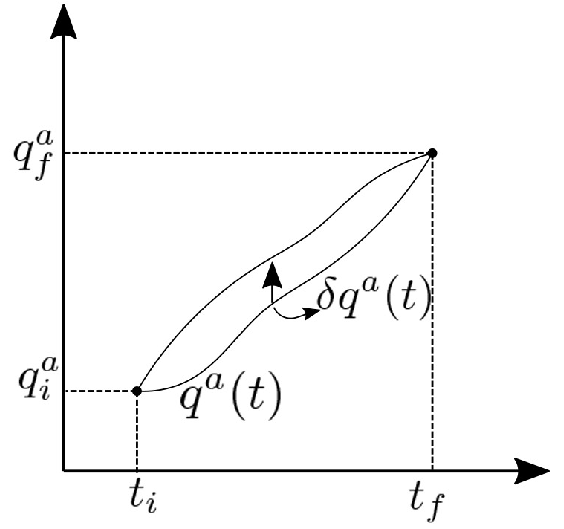
\includegraphics[width=8cm]{figura123.png}
	\caption{variación de la función $q(t)$.}
	\label{fig.1}
\end{figure}


donde $\delta q^a(t)$ es una \textit{variación} de la función $q^a(t)$ en el intervalo de $t_1$ a $t_2$. Puesto que para $t=t_i$ y $t=t_f$ todas las funciones (6.50) deben tomar el mismo valor 

\begin{equation}
\displaystyle \delta q^a(t_i)=\delta q^a(t_f)=0
\end{equation}

La variación de $I$ esta dada por:

\begin{eqnarray}
\delta I&=&\int_{t_i}^{t_f} \delta L \left( q,\dot{q},t \right) dt \\
&=& \int_{t_i}^{t_f} \left[ L \left( q + \delta q,\dot{q} + \delta \dot{q},t \right) - L \left( q,\dot{q},t \right) \right] dt \\
&=& \int_{t_i}^{t_f} \left[ L(q,\dot{q},t) + \frac{\partial L}{\partial q^a} \delta q^a + \frac{\partial L}{\partial \dot{q}^a} \delta \dot{q}^a - L(q.\dot{q},t) \right]dt \\
&=& \int_{t_i}^{t_f}  \left(\frac{\partial L}{\partial q^a} \delta q^a + \frac{\partial L}{\partial \dot{q}^a} \delta \dot{q}^a \right) dt 
\end{eqnarray}

considerando que $\delta \dot{q}^a = \displaystyle \frac{d}{dt} (\delta q^a)$

\begin{eqnarray}
\delta I &=& \int_{t_i}^{t_f} \left(\frac{\partial L}{\partial q^a} \delta q^a + \frac{\partial L}{\partial \dot{q}^a} \frac{d}{dt} (\delta q^a) \right) \\
&=& \int_{t_i}^{t_f} \left[ \frac{\partial L}{\partial q^a} \delta q^a + \frac{d}{dt} \left( \frac{\partial L}{\partial \dot{q}^a} \delta q^a \right)- \frac{d}{dt} \left( \frac{\partial L}{\partial \dot{q}^a} \right) \delta q^a   \right]dt \\
&=& \int_{t_i}^{t_f} \left\{ \left[  \frac{\partial L}{\partial q^a} - \frac{d}{dt} \left( \frac{\partial L}{\partial \dot{q}^a} \right) \right] \delta q^a + \frac{d}{dt} \left( \frac{\partial L}{\partial \dot{q}^a} \delta q^a \right) \right\} dt
\end{eqnarray}

Sea $\displaystyle \frac{\delta L}{\delta q^a}=\frac{\partial L}{\partial q^a}-\frac{d}{dt}\left( \frac{\partial L}{\partial \dot{q}^a} \right)$, luego:

\begin{eqnarray}
\delta I &=& \int_{t_i}^{t_f} \left[ \frac{\delta L}{\delta q^a} \delta q^a + \frac{d}{dt} \left( \frac{\partial L}{\partial \dot{q}^a}\delta q^a \right) \right] dt \\
&=&\int_{t_i}^{t_f}  \frac{\delta L}{\delta q^a} \delta q^a dt + \int_{t_1}^{t_2} \frac{d}{dt} \left( \frac{\partial L}{\partial \dot{q}^a}\delta q^a \right)  dt 
\end{eqnarray}

En virtud de las condiciones (6.51) y el enunciado anterior, tenemos que:

\begin{eqnarray}
\int_{t_i}^{t_f} \frac{\delta L}{\delta q^a} \delta q^a dt = 0 \\
\Rightarrow \frac{\delta L}{\delta q^a}\delta q^a =0
\end{eqnarray}

Pero el conjunto $\displaystyle\{ \delta q^a \}_{i=1}^f$ es linealmente independiente, por lo que obtenemos

\begin{equation}
\frac{\delta L}{\delta q^a}=0 \ \ \ \ a=1,...,f.
\end{equation}


Por tanto, las ecuaciones de movimiento de Euler-Lagrange son una condición para la validez del principio de Hamilton.













\section{No Unicidad de la función Lagrangiana}

Es importante señalar que el Lagrangiano no es unico. Pues para un sistema especifico existen muchas funciones Lagrangianas, las cuales arrojan el mismo conjunto de ecuaciones de movimiento, y que que representan igualmente la dinámica del sistema físico asociado. Consideremos la función $L$ definida por:

\begin{equation}
L\left(q,\dot{q},t\right)= \frac{d\Omega(q^a,t)}{dt}
\end{equation}

donde  $\Omega$ es una función arbitraria de las coordenadas y el el tiempo. Consideremos el siguiente conjunto de operadores diferenciales:

\begin{equation}
\frac{\delta}{\delta q^a} = \frac{d}{dt}\left( \frac{\partial}{\partial \dot{q}^a} \right) - \frac{\partial }{\partial q^a} \ \ \ ; \ \ \ a=1,...,f
\end{equation}

Aplicando el operador en el lagrangiano obtenemos:

\begin{eqnarray}
\frac{\delta}{\delta q^a} \left( \frac{d\Omega}{dt} \right) &=& \frac{d}{dt} \left[ \frac{\partial}{\partial \dot{q}^a} \left( \frac{d\Omega}{dt} \right) \right] -\frac{\partial}{\partial q^a} \left( \frac{d\Omega}{dt} \right) \\
&=& \frac{d}{dt} \left[ \frac{\partial}{\partial \dot{q}^a} \left( \frac{\partial \Omega}{\partial q^b} \dot{q^b} + \frac{\partial \Omega}{\partial t} \right)  \right] - \frac{\partial}{\partial q^a} \left( \frac{\partial \Omega}{\partial q^b}\dot{q^b} \right) - \frac{\partial}{\partial q^a} \left( \frac{d\Omega}{dt} \right) \\
&=& \frac{d}{dt} \left( \frac{\partial \Omega}{\partial q^b} \delta_{a}^b \right) - \frac{\partial^2\Omega}{\partial q^a \partial q^b} \dot{q}^b - \frac{\partial \Omega}{\partial q^b} \frac{\partial \dot{q}^b}{\partial q^a}-\frac{\partial^2 \Omega}{\partial q^a \partial t} \\
&=& \frac{d}{dt}\left(\frac{\partial \Omega}{\partial q^a} \right) - \left[ \frac{\partial }{\partial q^b} \left( \frac{\partial \Omega}{\partial q^a} \right)\dot{q}^b + \frac{\partial}{\partial t} \left( \frac{\partial \Omega}{\partial q^a} \right) \right] \\
&=& \frac{d}{dt}\left(\frac{\partial \Omega}{\partial q^a} \right) - \frac{d}{dt}\left(\frac{\partial \Omega}{\partial q^a} \right) \\
&=& 0
\end{eqnarray}


\textbf{Teorema:} Si dos lagrangianos $L_1$ y $L_2$ proporcionan las mismas ecuaciones del movimiento, entonces:
\begin{equation}
L_2 - L_1 = \frac{d\Omega(q^a,t)}{dt}.
\end{equation}


\textit{Demostración}: \\

Se tiene que 

\begin{eqnarray}
\frac{\delta}{\delta q^a} \left( L_2 - L_1 \right) = \frac{\delta}{\delta q^a} \left( \frac{d\Omega}{dt} \right) \equiv 0 \\
\Rightarrow \frac{\delta L_2}{\delta q^a} - \frac{\delta L_1}{\delta q^a} = 0
\end{eqnarray}

por tanto:

\begin{equation}
\frac{\delta L_2}{\delta q^a}=\frac{\delta L_1}{\delta q^a}.
\end{equation}


















\section{Curvas Geod\'esicas.}

\subsection{Ejemplo en $\mathbb{R}^{2}$.}


Ya vimos que podemos usar el calculo variacional para obtener las ecuaciones del movimiento. Pero esta no es la \'unica aplicaci\'on que 
tiene el calculo de variaciones. Como vimos, consiste en perturbar continuamente una curva (usando un parámetro) y encontrar la curva que 
extremize la acción. Así podemos usar el principio variacional para encontrar la curva de mínima distancia entre dos puntos. Veamos 
primero el siguiente ejemplo para entender la situación: \\

En el espacio Euclidiano $\mathbb{R}^{2}$ el elemento de linea esta dado por:
	\begin{equation*}
		ds^{2} = dx^{2} + dy^{2}
	\end{equation*}

Recordemeos que $s$ es la distancia entre dos puntos en el espacio. Sean $P$ y $Q$ dos puntos en $\mathbb{R}^{2}$, la distancia entre ellos está dada por:
	\begin{equation*}
		s = \int^{Q}_{P} ds = \int^{Q}_{P} \sqrt{dx^{2} + dy^{2}}
	\end{equation*}

Esta ser\'a nuestra acci\'on a extremar. \\

Ahora consideremos una curva cualquiera (con extremos en los puntos $P$ y $Q$) en el espacio, parametrizada con un parámetro 
$\lambda$, tal que:
	\begin{align*}
		x &= x \left( \lambda \right) \\
		y &= y \left( \lambda \right)
	\end{align*}

Luego, de la regla de la cadena tenemos que:
	\begin{align*}
		dx &= \frac{dx}{d\lambda} d\lambda \\
		dy &= \frac{dy}{d\lambda} d\lambda
	\end{align*}
	
definimos:
	\begin{align*}
		Q &= \left( x \left(\lambda_{f} \right) , y \left(\lambda_{f} \right) \right) \\
		P &= \left( x \left(\lambda_{i} \right) , y \left(\lambda_{i} \right) \right)
	\end{align*}
	
Usaremos la notaci\'on:
	\begin{align*}
		x' &= \frac{dx}{d\lambda} \\
		y' &= \frac{dy}{d\lambda}
	\end{align*}

Reemplazando esto en la acci\'on, tenemos:
	\begin{equation*}
		s = \int^{\lambda_{f}}_{\lambda_{i}} \sqrt{x'^{2} + y'^{2}}d\lambda
	\end{equation*}	
		
Ahora apliquemos la variaci\'on:
	\begin{align*}
		\delta s &= \delta \int^{\lambda_{f}}_{\lambda_{i}}  \sqrt{ x'^{2} + y'^{2} }d\lambda \\
				 &= \int^{\lambda_{f}}_{\lambda_{i}}  \delta \sqrt{ x'^{2} + y'^{2} }d\lambda \\
				 &= \int^{\lambda_{f}}_{\lambda_{i}}  \left( \frac{x' \delta x'}{\sqrt{ x'^{2} + y'^{2} }} + \frac{y' \delta y'}{\sqrt{ x'^{2} + y'^{2} }} \right) d\lambda \\
				 &= \int^{\lambda_{f}}_{\lambda_{i}}  \frac{x'}{\sqrt{ x'^{2} + y'^{2} }} \delta x' d\lambda 
				  + \int^{\lambda_{f}}_{\lambda_{i}}  \frac{y'}{\sqrt{ x'^{2} + y'^{2} }} \delta y' d\lambda
	\end{align*}

Trabajaremos con el termino:
	\begin{equation*}
		\int^{\lambda_{f}}_{\lambda_{i}}  \frac{x'}{\sqrt{ x'^{2} + y'^{2} }} \delta x' d\lambda  
	\end{equation*}

Recordemos que:
	\begin{equation*}
		\delta x'= \delta \frac{dx}{d\lambda} = \frac{d}{d\lambda} \left( \delta x \right) = \frac{d \delta x}{d\lambda}
	\end{equation*}

As\'i:
	\begin{equation*}
		\int^{\lambda_{f}}_{\lambda_{i}}  \frac{x'}{\sqrt{ x'^{2} + y'^{2} }} \delta x' d\lambda =  \int^{\lambda_{f}}_{\lambda_{i}}  \frac{x'}{\sqrt{ x'^{2} + y'^{2} }} \frac{d \delta x}{d\lambda} d\lambda 
	\end{equation*}

Veamos que:
	\begin{equation*}
		\frac{x'}{\sqrt{ x'^{2} + y'^{2} }} \frac{d \delta x}{d\lambda} = \frac{d}{d\lambda} \left( \frac{x'}{\sqrt{ x'^{2} + y'^{2} }} \delta x  \right) 
																		  - \frac{d}{d\lambda} \left( \frac{x'}{\sqrt{ x'^{2} + y'^{2} }}  \right) \delta x 
	\end{equation*}

Luego:
	\begin{align*}
		\int^{\lambda_{f}}_{\lambda_{i}}  \frac{x'}{\sqrt{ x'^{2} + y'^{2} }} \frac{d \delta x}{d\lambda} d\lambda 
		  &= \int^{\lambda_{f}}_{\lambda_{i}}  \frac{d}{d\lambda} \left( \frac{x'}{\sqrt{ x'^{2} + y'^{2} }} \delta x  \right) d\lambda
	   	  - \int^{\lambda_{f}}_{\lambda_{i}}  \frac{d}{d\lambda} \left( \frac{x'}{\sqrt{ x'^{2} + y'^{2} }}  \right) \delta x d\lambda \\
	   	  &= \left( \frac{x'}{\sqrt{ x'^{2} + y'^{2} }} \delta x \right) \Big|^{\lambda_{f}}_{\lambda_{i}} - \int^{\lambda_{f}}_{\lambda_{i}}  \frac{d}{d\lambda} \left( \frac{x'}{\sqrt{ x'^{2} + y'^{2} }}  \right) \delta x d\lambda \\
	\end{align*}

Y como:
	\begin{equation*}
		\delta x (\lambda_{f}) = \delta x (\lambda_{i}) = 0 
	\end{equation*}

Obtenemos:
	\begin{align*}
		\int^{\lambda_{f}}_{\lambda_{i}}  \frac{x'}{\sqrt{ x'^{2} + y'^{2} }} \frac{d \delta x}{d\lambda} d\lambda = - \int^{\lambda_{f}}_{\lambda_{i}}  \frac{d}{d\lambda} \left( \frac{x'}{\sqrt{ x'^{2} + y'^{2} }}  \right) \delta x d\lambda 
	\end{align*}

Por tanto:
	\begin{align*}
		\int^{\lambda_{f}}_{\lambda_{i}}  \frac{x'}{\sqrt{ x'^{2} + y'^{2} }} \delta x' d\lambda = - \int^{\lambda_{f}}_{\lambda_{i}}  \frac{d}{d\lambda} \left( \frac{x'}{\sqrt{ x'^{2} + y'^{2} }}  \right) \delta x d\lambda 
	\end{align*}
	
Analogamente:
	\begin{align*}
		\int^{\lambda_{f}}_{\lambda_{i}}  \frac{y'}{\sqrt{ x'^{2} + y'^{2} }} \delta y' d\lambda = - \int^{\lambda_{f}}_{\lambda_{i}}  \frac{d}{d\lambda} \left( \frac{y'}{\sqrt{ x'^{2} + y'^{2} }}  \right) \delta y d\lambda 
	\end{align*}

Por lo que:
	\begin{equation*}
		\delta s = - \int^{\lambda_{f}}_{\lambda_{i}}  \frac{d}{d\lambda} \left( \frac{x'}{\sqrt{ x'^{2} + y'^{2} }}  \right) \delta x d\lambda  - \int^{\lambda_{f}}_{\lambda_{i}}  \frac{d}{d\lambda} \left( \frac{y'}{\sqrt{ x'^{2} + y'^{2} }}  \right) \delta y d\lambda 
	\end{equation*}	

Si pedimos que $\delta s = 0$ (buscamos los extremos), tenemos que:
	\begin{align*}
		- \int^{\lambda_{f}}_{\lambda_{i}}  \frac{d}{d\lambda} \left( \frac{x'}{\sqrt{ x'^{2} + y'^{2} }}  \right) \delta x d\lambda  - \int^{\lambda_{f}}_{\lambda_{i}}  \frac{d}{d\lambda} \left( \frac{y'}{\sqrt{ x'^{2} + y'^{2} }}  \right) \delta y d\lambda = 0
	\end{align*}

Y como $\delta x$ y  $\delta y$ son linealmente independientes, tenemos que:
	\begin{align*}
		\frac{d}{d\lambda} \left( \frac{x'}{\sqrt{ x'^{2} + y'^{2} }}  \right) &= 0 \\
		\frac{d}{d\lambda} \left( \frac{y'}{\sqrt{ x'^{2} + y'^{2} }}  \right) &= 0
	\end{align*}

De donde:
	\begin{align*}
		 \frac{x'}{\sqrt{ x'^{2} + y'^{2} }}  &= A \\
		 \frac{y'}{\sqrt{ x'^{2} + y'^{2} }}  &= B
	\end{align*}

Con $A$ y $B$ constantes. Dividimos las expresiones y obtenemos:
	\begin{align*}
		\frac{y'}{x'} = C
	\end{align*}

Y como:
	\begin{equation*}
		\frac{y'}{x'} = \frac{dy/d\lambda}{dx/d\lambda} = \frac{dy}{d\lambda} \frac{d\lambda}{dx} = \frac{dy}{dx}
	\end{equation*}

Finalmente:
	\begin{align*}
		\frac{dy}{dx} &= C \\
		\Rightarrow y &= Cx + D
	\end{align*}
	
Lo que corresponde a una recta. \\

En resumen, perturbamos una curva en el espacio Euclidiano $\mathbb{R}^{2}$ y aplicamos el principio variacional para encontrar la curva de 
longitud mínima entre dos puntos, obteniendo as\'i una recta, lo cual era el resultado esperado. \\

\textbf{Nota:} El calculo fue realizado de la manera m\'as general posible, no necesariamente siendo esto la manera m\'as \'optima de 
aplicar la variaci\'on. Sugerimos rehacer el calculo, pero esta vez, usando el teorema de la funci\'on implicita, para obtener la ecuaci\'on 
de la curva de la forma $y=y(x)$, y luego hacer variar la acci\'on. Se dar\'a cuenta de que realizar el calculo de esta forma es mucho m\'as 
sencillo (pero no tan general). \\



\subsection{Curvas Geod\'esicas en cualquier espacio.}

Una vez entendido la manera de abordar este problema, nos gustar\'ia saber cual es la curva de mínima longitud que une dos puntos, 
esta vez no necesariamente en $\mathbb{R}^{2}$, sino que, en \textbf{cualquier espacio}, de \textbf{cualquier dimensi\'on}. \\

Empecemos considerando un espacio de $n$ dimensiones, con una m\'etrica $g_{ij}$, donde $i,j = 1,...,n$. El elemento de linea en este espacio 
esta dado por:
	\begin{equation*}
		ds^{2} = g_{ij}dx^{i}dx^{j}
	\end{equation*}

Como en el ejemplo, consideremos dos puntos ($P$ y $Q$) en el espacio, la distancia entre ellos esta dada por:
	\begin{equation*}
		s = \int^{Q}_{P} ds = \int^{Q}_{P} \sqrt{g_{ij}dx^{i}dx^{j}}
	\end{equation*}

Siguiendo con la metodolog\'ia usada en el ejemplo, consideremos una curva en el espacio, que tiene por extremos los puntos $P$ y $Q$, 
y que ademas esta parametrizada con un parámetro $\lambda$, tal que:
	\begin{equation*}
		x^{i} = x^{i} (\lambda)
	\end{equation*}

De donde:
	\begin{equation*}
		dx^{i} = \frac{dx^{i}}{d\lambda} d\lambda = x'^{i}d\lambda
	\end{equation*}
	
Y definimos:
	\begin{align*}
		Q &= \left( x^{1} \left(\lambda_{f} \right) ,...,  x^{n} \left(\lambda_{f} \right) \right) \\
		P &= \left( x^{1} \left(\lambda_{i} \right) ,...,  x^{n} \left(\lambda_{i} \right) \right)
	\end{align*}
	
Notemos que:
	\begin{equation*}
		\frac{ds}{d\lambda} = \sqrt{g_{ij}x'^{i}x'^{j}}
	\end{equation*}

Reemplazando en la acci\'on:
	\begin{equation*}
		s = \int^{\lambda_{f}}_{\lambda{i}} \sqrt{g_{ij}x'^{i}x'^{j}} d\lambda
	\end{equation*}

Aplicando la varici\'on:
	\begin{align*}
		\delta s &= \delta\int^{\lambda_{f}}_{\lambda{i}} \sqrt{g_{ij}x'^{i}x'^{j}} d\lambda \\
				 &= \int^{\lambda_{f}}_{\lambda{i}} \delta \sqrt{g_{ij}x'^{i}x'^{j}} d\lambda \\
				 &= \int^{\lambda_{f}}_{\lambda{i}} \frac{\delta\left( g_{ij}x'^{i}x'^{j} \right)}{2\sqrt{g_{ab}x'^{a}x'^{b}}} d\lambda \\
				 &= \int^{\lambda_{f}}_{\lambda{i}} \frac{\delta g_{ij}x'^{i}x'^{j} + 2g_{ij}x'^{i}\delta x'^{j}}{2\sqrt{g_{ab}x'^{a}x'^{b}}} d\lambda \\
	\end{align*}
	
Notemos que:
	\begin{equation*}
		\delta g_{ij} = \frac{\partial g_{ij}}{\partial x^{k}} \delta x^{k}
	\end{equation*}
	
As\'i: 
	\begin{align*}
		\delta s &= \int^{\lambda_{f}}_{\lambda{i}} \frac{1}{2\sqrt{g_{ab}x'^{a}x'^{b}}} \left(  \frac{\partial g_{ij}}{\partial x^{k}}x'^{i}x'^{j} \delta x^{k} + 2g_{ij}x'^{i}\delta x'^{j} \right) d\lambda \\
				 &= \int^{\lambda_{f}}_{\lambda{i}} \left( \frac{\frac{\partial g_{ij}}{\partial x^{k}}x'^{i}x'^{j}}{2\sqrt{g_{ab}x'^{a}x'^{b}}} \delta x^{k}
				                                        +  \frac{g_{ij}x'^{i}\delta x'^{j}}{\sqrt{g_{ab}x'^{a}x'^{b}}} \right) d\lambda 
	\end{align*}

Veamos el termino:
	\begin{equation*}
		\frac{g_{ij}x'^{i}\delta x'^{j}}{\sqrt{g_{ab}x'^{a}x'^{b}}}
	\end{equation*}

Recordemos que:
	\begin{equation*}
		\delta x'^{i} = \frac{d \delta x^{i}}{d\lambda}
	\end{equation*}

As\'i:
	\begin{align*}
		\frac{g_{ij}x'^{i}\delta x'^{j}}{\sqrt{g_{ab}x'^{a}x'^{b}}} &= \frac{g_{ij}x'^{i}}{\sqrt{g_{ab}x'^{a}x'^{b}}}\frac{d \delta x^{j}}{d\lambda} \\
																	&= \frac{d}{d\lambda} \left(\frac{g_{ij}x'^{i}}{\sqrt{g_{ab}x'^{a}x'^{b}}} \delta x^{j}\right) 
																	 - \frac{d}{d\lambda} \left( \frac{g_{ij}x'^{i}}{\sqrt{g_{ab}x'^{a}x'^{b}}} \right)\delta x^{j}
	\end{align*}
	
Luego:
	\begin{align*}
		\int^{\lambda_{f}}_{\lambda{i}} \frac{g_{ij}x'^{i}\delta x'^{j}}{\sqrt{g_{ab}x'^{a}x'^{b}}} d\lambda
			&= \int^{\lambda_{f}}_{\lambda{i}} \frac{d}{d\lambda} \left(\frac{g_{ij}x'^{i}}{\sqrt{g_{ab}x'^{a}x'^{b}}} \delta x^{j}\right) d\lambda
			 - \int^{\lambda_{f}}_{\lambda{i}} \frac{d}{d\lambda} \left( \frac{g_{ij}x'^{i}}{\sqrt{g_{ab}x'^{a}x'^{b}}} \right)\delta x^{j} d\lambda \\
			&= \left( \frac{g_{ij}x'^{i}}{\sqrt{g_{ab}x'^{a}x'^{b}}} \delta x^{j} \right) \Big|^{\lambda_{f}}_{\lambda_{i}} 
			- \int^{\lambda_{f}}_{\lambda{i}} \frac{d}{d\lambda} \left( \frac{g_{ij}x'^{i}}{\sqrt{g_{ab}x'^{a}x'^{b}}} \right) \delta x^{j} d\lambda
	\end{align*}
	
Y como:
	\begin{equation*}
		\delta x^{i} (\lambda_{i}) = \delta x^{i} = 0
	\end{equation*}

Tenemos que:
	\begin{equation*}
		\int^{\lambda_{f}}_{\lambda{i}} \frac{g_{ij}x'^{i}\delta x'^{j}}{\sqrt{g_{ab}x'^{a}x'^{b}}} d\lambda
			= - \int^{\lambda_{f}}_{\lambda{i}} \frac{d}{d\lambda} \left( \frac{g_{ij}x'^{i}}{\sqrt{g_{ab}x'^{a}x'^{b}}} \right) \delta x^{j} d\lambda
	\end{equation*}
		
Luego:
	\begin{align*}
		\delta s &= \int^{\lambda_{f}}_{\lambda{i}} \left( \frac{\frac{\partial g_{ij}}{\partial x^{k}}x'^{i}x'^{j}}{2\sqrt{g_{ab}x'^{a}x'^{b}}} \delta x^{k}
				                                        -  \frac{d}{d\lambda} \left( \frac{g_{ij}x'^{i}}{\sqrt{g_{ab}x'^{a}x'^{b}}} \right) \delta x^{j} \right) d\lambda \\ 
				 &= \int^{\lambda_{f}}_{\lambda{i}} \frac{1}{\sqrt{g_{ab}x'^{a}x'^{b}}} \left( \frac{1}{2}\frac{\partial g_{ij}}{\partial x^{k}} x'^{i}x'^{j} \delta x^{k}
				                                        -  \sqrt{g_{cd}x'^{c}x'^{d}}\frac{d}{d\lambda} \left( \frac{g_{ij}x'^{i}}{\sqrt{g_{ef}x'^{e}x'^{f}}} \right) \delta x^{j} \right) d\lambda \\ 
				 &= \int^{\lambda_{f}}_{\lambda{i}} \frac{1}{\sqrt{g_{ab}x'^{a}x'^{b}}} \left( \frac{1}{2}\frac{\partial g_{ij}}{\partial x^{k}} x'^{i}x'^{j} \delta x^{k}
				                                        - \frac{d}{d\lambda} \left( g_{ij}x'^{i} \right) \delta x^{j}  
				                                        + \frac{g_{ij}x'^{i}}{\sqrt{g_{ef}x'^{e}x'^{f}}} \frac{d}{d\lambda} \left( \sqrt{g_{cd}x'^{c}x'^{d}} \right) \delta x^{j} 
														\right) d\lambda\\
				&= 	\int^{\lambda_{f}}_{\lambda{i}} \frac{1}{\sqrt{g_{ab}x'^{a}x'^{b}}} \left( \frac{1}{2}\frac{\partial g_{ij}}{\partial x^{k}} x'^{i}x'^{j} \delta x^{k}
				                                        - \frac{\partial g_{ij}}{\partial x^{k}} x'^{i} x'^{k}\delta x^{j} - g_{ij}x''^{i}\delta x^{j}  
				                                        + \frac{g_{ij}x'^{i}}{\sqrt{g_{ef}x'^{e}x'^{f}}} \frac{d}{d\lambda} \left( \sqrt{g_{cd}x'^{c}x'^{d}} \right) \delta x^{j} 
														\right) d\lambda										
	\end{align*}
	
Notemos que:
	\begin{equation*}
		\frac{1}{\sqrt{g_{ef}x'^{e}x'^{f}}} \frac{d}{d\lambda} \left( \sqrt{g_{cd}x'^{c}x'^{d}} \right)
		=  \frac{d}{d\lambda} \left( \ln \left( \sqrt{g_{cd}x'^{c}x'^{d}} \right) \right)
	\end{equation*}

Definiendo:
	\begin{equation*}
		\alpha(s) = \frac{d}{d\lambda} \left( \ln \left( \sqrt{g_{cd}x'^{c}x'^{d}} \right) \right)
	\end{equation*}
	
Reemplazando en $\delta s$ y cambiando el indice de suma:
	\begin{equation*}
		\delta s =  \int^{\lambda_{f}}_{\lambda{i}} \frac{1}{\sqrt{g_{ab}x'^{a}x'^{b}}} \left( \frac{1}{2}\frac{\partial g_{ij}}{\partial x^{k}} x'^{i}x'^{j} 
			                                       - \frac{\partial g_{ik}}{\partial x^{j}} x'^{i} x'^{j} - g_{ik}x''^{i} 
				                                        + \alpha\left( s \right) g_{ik}x'^{i} 
														\right) \delta x^{k}  d\lambda	
	\end{equation*}
	

	
Notemos que (ejercicio):
	\begin{equation*}
		\frac{\partial g_{ik}}{\partial x^{j}} x'^{i} x'^{j} = \frac{1}{2} \left( \frac{\partial g_{ik}}{\partial x^{j}} + \frac{\partial g_{jk}}{\partial x^{i}} \right) x'^{i}x'^{j}
	\end{equation*}


Reemplazando lo anterior:
	\begin{align*}
		\delta s &=  \int^{\lambda_{f}}_{\lambda{i}} \frac{1}{\sqrt{g_{ab}x'^{a}x'^{b}}} \left( \frac{1}{2}\frac{\partial g_{ij}}{\partial x^{k}} x'^{i}x'^{j} 
				                                    - \frac{1}{2} \left( \frac{\partial g_{ik}}{\partial x^{j}} + \frac{\partial g_{jk}}{\partial x^{i}} \right) x'^{i}x'^{j} - g_{ik}x''^{i} 
				                                        + \alpha\left( s \right) g_{ik}x'^{i} 
														\right) \delta x^{k}  d\lambda\\	
				 &=  \int^{\lambda_{f}}_{\lambda{i}} \frac{1}{\sqrt{g_{ab}x'^{a}x'^{b}}} \left( 
													\frac{1}{2}\frac{\partial g_{ij}}{\partial x^{k}} x'^{i}x'^{j} 
				                                    - \frac{1}{2}\frac{\partial g_{ik}}{\partial x^{j}}x'^{i}x'^{j} - \frac{1}{2}\frac{\partial g_{jk}}{\partial x^{i}} x'^{i}x'^{j} - g_{ik}x''^{i} 
				                                        + \alpha\left( s \right) g_{ik}x'^{i} 
														\right) \delta x^{k}  d\lambda \\
				 &=  \int^{\lambda_{f}}_{\lambda{i}} \frac{1}{\sqrt{g_{ab}x'^{a}x'^{b}}} \left( - g_{ik}x''^{i}
													-\frac{1}{2}\left( \frac{\partial g_{ik}}{\partial x^{j}} + \frac{\partial g_{jk}}{\partial x^{i}}-\frac{\partial g_{ij}}{\partial x^{k}} \right)x'^{i}x'^{j}
				                                        + \alpha \left( s \right) g_{ik}x'^{i} 
														\right) \delta x^{k}  d\lambda \\
				 &=  \int^{\lambda_{f}}_{\lambda{i}} \frac{1}{\sqrt{g_{ab}x'^{a}x'^{b}}} \left( - g_{il}x''^{i}
													-\frac{1}{2}\left( \frac{\partial g_{kl}}{\partial x^{j}} + \frac{\partial g_{jl}}{\partial x^{k}}-\frac{\partial g_{kj}}{\partial x^{l}} \right)x'^{j}x'^{k}
				                                        + \alpha\left( s \right) g_{il}x'^{i} 
														\right) \delta x^{l}  d\lambda \\	
				 &=  \int^{\lambda_{f}}_{\lambda{i}} \frac{1}{\sqrt{g_{ab}x'^{a}x'^{b}}} \left( - g_{il}x''^{i}
													-\frac{1}{2}\delta^{m}_{l}\left( \frac{\partial g_{km}}{\partial x^{j}} + \frac{\partial g_{jm}}{\partial x^{k}}-\frac{\partial g_{kj}}{\partial x^{m}} \right)x'^{j}x'^{k}
				                                        + \alpha\left( s \right) g_{il}x'^{i} 
														\right) \delta x^{l}  d\lambda \\																																												
	\end{align*}

Pero:
	\begin{equation*}
		\delta^{m}_{l} = g_{il}g^{im}
	\end{equation*}

Tenemos que:
	\begin{align*}
		\delta s &=  \int^{\lambda_{f}}_{\lambda{i}} \frac{1}{\sqrt{g_{ab}x'^{a}x'^{b}}} \left( - g_{il}x''^{i}
													-\frac{1}{2}g_{il}g^{im}\left( \frac{\partial g_{km}}{\partial x^{j}} + \frac{\partial g_{jm}}{\partial x^{k}}-\frac{\partial g_{kj}}{\partial x^{m}} \right)x'^{j}x'^{k}
				                                        + \alpha\left( s \right) g_{il}x'^{i} 
														\right) \delta x^{l}  d\lambda \\
			     &=  \int^{\lambda_{f}}_{\lambda{i}} \frac{g_{il}}{\sqrt{g_{ab}x'^{a}x'^{b}}} \left( - x''^{i}
													-\frac{1}{2}g^{im}\left( \frac{\partial g_{km}}{\partial x^{j}} + \frac{\partial g_{jm}}{\partial x^{k}}-\frac{\partial g_{kj}}{\partial x^{m}} \right)x'^{j}x'^{k}
				                                        + \alpha\left( s \right) x'^{i} 
														\right) \delta x^{l}  d\lambda \\																																												
	\end{align*}
	
Recordando que el simbolo de Christofell se define como:
	\begin{equation*}
		\Gamma^{i}_{jk} = \frac{1}{2} g^{im} \left( \frac{\partial g_{km}}{\partial x^{j}} + \frac{\partial g_{jm}}{\partial x^{k}}-\frac{\partial g_{kj}}{\partial x^{m}}    \right)
	\end{equation*}
	
Finalmente obtenemos que:
	\begin{equation*}
		\delta s =  \int^{\lambda_{f}}_{\lambda{i}} \frac{g_{il}}{\sqrt{g_{ab}x'^{a}x'^{b}}} \left( - x''^{i}
													-\Gamma^{i}_{jk} x'^{j}x'^{k} + \alpha\left( s \right) x'^{i} 
														\right) \delta x^{l}  d\lambda 																																											
	\end{equation*}
	
Pidiendo que $\delta s = 0$ y considerando que los $\delta x^{i}$ son linealmente independiente, obtenemos que:
	\begin{equation*}
		x''^{i} + \Gamma^{i}_{jk} x'^{j}x'^{k} = \alpha\left( s \right) x'^{i}
	\end{equation*}

Esta es llamada \textbf{Ecuaci\'on de la Geod\'esica}, esta es la curva de mínima longitud entre dos puntos, que esta parametrizada 
con un parámetro cualquiera $\lambda$. Pero esta ecuaci\'on puede ser bastante dif\'icil de resolver debido a la funci\'on $\alpha(s)$. 
Debido a esto, ser\'ia bastante cómodo que esta funci\'on fuera igual a cero. Veamos que pasa si pedimos esa condici\'on:
	\begin{align*}
		\alpha(s) &= 0 \\
		\Rightarrow \frac{d}{d\lambda} \left( \ln \left( g_{ab} x'^{a}x'^{b}\right) \right) &= 0 \\
		\Rightarrow \frac{d}{d\lambda} \left( \ln \left( \frac{ds}{d\lambda }\right) \right) &= 0 \\
		\Rightarrow \frac{d\lambda}{ds}\frac{d^{2}s}{d\lambda^{2}} &= 0 \\
		\Rightarrow \frac{d^{2}s}{d\lambda^{2}} &= 0 \\
		\Rightarrow s &= a \lambda + b \\  
		\Rightarrow \lambda &= \frac{s}{a} - b \\
	\end{align*}

La longitud de arco $s$ puede ser usada como par\'ametro a lo largo de la curva. A $s$ se le llama par\'ametro natural, y a $x^{i} = x^{i}(s)$ 
se le llama parametrizaci\'on natural. Para el par\'ametro natural usaremos la siguiente notaci\'on:
	\begin{equation*}
		\dot{x}^{i} = \frac{dx^{i}}{ds}
	\end{equation*}

Si una curva esta parametrizada con el par\'ametro natural se cumple que:
	\begin{equation*}
		 \sqrt{g_{ij}\dot{x}^{i} \dot{x}^{j}} = 1
	\end{equation*}

Notemos que:
	\begin{align*}
		\frac{d}{d\lambda} &= \frac{d}{ds}\frac{ds}{d\lambda} \\ 
						   &= a\frac{d}{ds} \\
		\Rightarrow x'^{i} &= a \dot{x}^{i} \\
		\Rightarrow x''^{i} &= a^{2} \ddot{x}^{i} \\
 	\end{align*}
	
Reemplazando en la ecuaci\'on de la geod\'esica	obtenemos:
	\begin{equation*}
		\ddot{x}^{i} + \Gamma^{i}_{jk} \dot{x}^{j}\dot{x}^{k} = 0
	\end{equation*}

Que corresponde a la \textbf{ Ecuaci\'on de la Geod\'esica Af\'in}.







































\section{Caso Electromagnetico}  
 


Un caso de interes es la obtención del lagrangiano de una particula sometida a un campo electromagnetico. \\

La fuerza sobre una carga q es dada por:

\begin{equation}
\vec{F} = q\vec{E} + q\vec{v} \times \vec{B}
\end{equation}

Consideremos las siguientes ecuaciones:

\begin{eqnarray}
\vec{\nabla} \cdot \vec{B} = 0 \\
\frac{\partial \vec{B}}{\partial t} + \vec{\nabla} \times \vec{E} = 0
\end{eqnarray}


de la ecuación (6.77) podemos ver que existe un potencial $\vec{A}$ tal que 

\begin{equation}
\vec{B} = \vec{\nabla} \times \vec{A}
\end{equation}
 
 introduciendo (6.79) en (6.78) obtenemos
 
\begin{eqnarray}
\frac{\partial }{\partial t} \left( \vec{\nabla} \times \vec{A} \right) + \vec{\nabla} \times \vec{E} =0 \\
\vec{\nabla} \times \frac{\partial \vec{A}}{\partial t} + \vec{\nabla} \times \vec{E} =0 \\
\vec{\nabla} \left( \frac{\partial \vec{A}}{\partial t} + \vec{E} \right) = 0 \\
\Rightarrow \frac{\partial \vec{A}}{\partial t} + \vec{E} = - \vec{\nabla} \phi \\
\vec{E} = -\vec{\nabla}\phi - \frac{\partial \vec{A}}{\partial t}
\end{eqnarray}


Reemplazando (6.84) en (6.76) obtenemos

\begin{eqnarray}
\vec{F}= -q \left( \vec{\nabla} \phi + \frac{\partial \vec{A}}{\partial t} \right) + q\vec{v} \times \vec{\nabla} \times \vec{A}
\end{eqnarray}


considerando que $\vec{A}=\vec{A}(\vec{x},t)$, tenemos:

\begin{eqnarray}
\frac{d\vec{A}}{dt}&=& \frac{\partial \vec{A}}{\partial x}\frac{dx}{dt} + \frac{\partial \vec{A}}{\partial y}\frac{dy}{dt} + \frac{\partial \vec{A}}{\partial z}\frac{dz}{dt} + \frac{\partial A}{\partial t} \\
 \frac{d\vec{A}}{dt}&=& \left( \frac{d\vec{x}}{dt} \cdot \vec{\nabla} \right) \vec{A} + \frac{\partial \vec{A}}{\partial t}
\end{eqnarray}



por otra parte, del calculo vectorial sabemos que 

\begin{eqnarray}
\vec{v} \times \vec{\nabla} \times \vec{A} &=& \vec{\nabla} \left(\vec{v} \cdot \vec{A} \right)- \left(\vec{v} \cdot \vec{\nabla}\right) \vec{A} \\
&=& \vec{\nabla} \left(\vec{v} \cdot \vec{A}\right) - \left( \frac{d\vec{A}}{dt}-\frac{\partial \vec{A}}{\partial t} \right)
\end{eqnarray}

reemplzando (6.89) en (6.85) obtenemos

\begin{eqnarray}
\vec{F} &=&= -q\vec{\nabla}\phi - \cancel{q\frac{\partial A}{\partial t}} + q\vec{\nabla} \left( \vec{v} \cdot \vec{A} \right) - q\frac{d\vec{A}}{dt} + \cancel{q\frac{\partial \vec{A}}{\partial t}} \\
&=&  -q\vec{\nabla}\phi  + q\vec{\nabla} \left(\vec{v} \cdot \vec{A} \right) - q\frac{d\vec{A}}{dt} 
\end{eqnarray}


dado que $ \vec{A}=\displaystyle \vec{\nabla}_{\vec{v}} \left( \vec{v} \cdot \vec{A} \right) \equiv \frac{\partial}{\partial v_i} \left( \vec{v} \cdot \vec{A} \right)$


\begin{eqnarray}
\vec{F}&=&q\left(- \vec{\nabla}\phi +\vec{\nabla} \left( \vec{A} \cdot \vec{v} \right) - \frac{d}{dt} \left[ \vec{\nabla}_{\vec{v}} \left( \vec{v} \cdot \vec{A} \right)  \right] \right) \\
&=& q \left( -\nabla \left( \phi-\vec{v} \cdot \vec{A} \right) - \frac{d}{dt} \left[ \vec{\nabla}_{\vec{v}} \left( \vec{v} \cdot \vec{A} \right) \right] \right) \\
&=& -\vec{\nabla} \left[ q\left( \phi - \vec{v} \cdot \vec{A}  \right) \right] - \frac{d}{dt} \left[ \vec{\nabla}_{\vec{v}} \left( q\vec{v} \cdot \vec{A} \right) \right]
\end{eqnarray}


notemos que $\phi=\phi(\vec{x}) \Rightarrow \vec{\nabla}_{\vec{v}}\left(\phi\right)=0$, luego

\begin{eqnarray}
\vec{F}&=&-\vec{\nabla} \left[ q\left( \phi - \vec{v} \cdot \vec{A}  \right) \right] +\frac{d}{dt} \left[\vec{\nabla}_{\vec{v}}\left( q\phi \right) \right] - \frac{d}{dt} \left[ \vec{\nabla}_{\vec{v}} \left( q\vec{v} \cdot \vec{A} \right) \right] \\
&=& \frac{d}{dt}\left[ \vec{\nabla}_{\vec{v}} \left( q \left[ \phi - \vec{v} \cdot \vec{A} \right] \right) \right] - \vec{\nabla} \left[ q \left( \phi - \vec{v} \cdot \vec{A} \right) \right]
\end{eqnarray}

por tanto, el lagrangiano para una particula con carga sometida a un campo electromagnetico esta dado por:

\begin{equation}
L=\frac{1}{2}mv^2 - q\phi + q\vec{A} \cdot \vec{v}
\end{equation}













\section{Teoremas de Conservación}

Hasta el momento los métodos que hemos estudiado nos permiten encontrar las ecuaciones diferenciales que determinan la dinámica de un sistema físico con $f$ grados de libertad. Como estas ecuaciones son de segundo orden se requieren $2f$ constantes de integración (o constates de movimiento) que usualmente se determinan con las condiciones iniciales del problema. \\


La solución completa de una ecuación de segundo orden requiere formalmente de dos procesos de integración, con frecuencia el primer proceso de integración es mas fácil, pero el ultimo proceso no se puede llevar a cabo tan fácilmente. En otras palabras, podemos obtener una ecuación de la forma

\begin{equation}
f(q,\dot{q},t) = cte
\end{equation}

las cuales son ecuaciones diferenciales de primer orden. Mucha información se puede obtener a partir de estas, en particular las leyes de conservación.\\

Consideremos un sistema de partículas puntuales bajo la acción de fuerzas que se derivan de potenciales que solo dependen de la posición. En este caso se tiene que

\begin{eqnarray}
\frac{\partial L}{\partial \dot{x}_i}&=&\frac{\partial T}{\partial \dot{x}_i} - \frac{\partial U}{\partial \dot{x}_i} = \frac{\partial T}{\partial \dot{x}_i} \\
 \frac{\partial L}{\partial \dot{x}_i}&=& \frac{\partial }{\partial \dot{x}_i} \sum_{k} \frac{1}{2} m_k \left( \dot{x}_k^2 + \dot{y}_k^2  + \dot{z}_k^2  \right)  \\
 \frac{\partial L}{\partial \dot{x}_i} &=& m_i \dot{x}_i = p_{x_i}
\end{eqnarray} 


corresponde a la componente $x$ del momento lineal de la partícula i-ésima.
De manera análoga podemos definir el \textit{momento generalizado} $p_a$ asociado a la coordenada generalizada $q^a$ como

\begin{equation}
p_a  \equiv \frac{\partial L}{\partial \dot{q}^a}
\end{equation}

\underline{Nota}: toda variable que involucre cambio tiene un momento canonico conjugado. \\

\textbf{Ejemplo:} Consideremos el Lagrangiano $L=\displaystyle\frac{1}{2}m \left( \dot{r}^2 + r^2\dot{\phi}^2 \right)$. Podemos ver que 


\begin{eqnarray}
p_{r} &=& \frac{\partial L}{\partial \dot{r}} = m \dot{r} \\
\\
p_{\phi} &=&\frac{\partial L}{\partial \dot{\phi}} = mr^2 \dot{\phi}.
\end{eqnarray}

Notemos que $p_a$ no tiene necesariamente dimensiones  de momento lineal. Cuando tenemos potenciales dependientes de la velocidad el momento generalizada difiere del momento mecánico. Un ejemplo claro de esto es el de una partícula en un campo electromagnético, cuyo Lagrangiano fue obtenido en la sección anterior.

\begin{equation}
L=\frac{1}{2}mv^2 - q\phi + q \vec{A} \cdot \vec{v} 
\end{equation}

donde en este caso $q$ denota carga eléctrica. El momento generalizado es 

\begin{equation}
\vec{p}=m \vec{x} + q\vec{A}
\end{equation}


que es el momento mecánico asociado a la partícula mas un termino adicional que depende del campo. \\ 

En algunas ocasiones el Lagrangiano no depende de alguna coordenada $q^a$, pero si depende de su velocidad generalizada asociada $\dot{q}^a$. En este caso se dice que $q^a$ es una coordenada \textbf{cíclica} o \textbf{ignorable}, luego la ecuación asociada a esta coordenada se reduce a 

\begin{equation}
\frac{d}{dt} \left( \frac{\partial L}{\partial \dot{q}^a} \right) = 0
\end{equation}

se puede observar que 

\begin{equation}
\frac{dp_a}{dt} = 0 \Rightarrow p_a = cte
\end{equation}

de lo cual resulta el siguiente teorema de conservación: \textbf{ el momento canónico $p_{a}$ conjugado en la coordenada $q^a$ se conserva si $q^a$ es ciclica }. \\


Los momentos generalizados conservados constituyen primeras integrales de movimiento, pues al pasar de (6.108) a (6.109) hemos pasado de una ecuación diferencial de primer orden a una de primer orden, lo cual equivale a hacer una integración. \\




\subsection{Función Energía y Conservación de la Energía}


Una interrogante esperable en nuestro estudio es si el teorema de conservación de la energía se pueda obtener a partir del formalismo Lagrangiano. Ya hemos visto que la ausencia de una coordenada generalizada en el Lagrangiano conduce a la conservación de un momento generalizado, en efecto, es natural entonces preguntarse si la ausencia de la  variable tiempo conduce a algún teorema de conservación. La analogía no es tan directa ya que no hemos asociado un momento generalizado con la variable tiempo ni tiene sentido tampoco una variable $\dot{t}$, en ese sentido no podemos hablar del tiempo como una coordenada generalizada. Más bien, el tiempo se considera como un parámetro que ademas de aparecer explícitamente, regula la evolución de las coordenadas. 


Al igual que en el caso de los momentos, veremos que del formalismo Lagrangiano sale un  teorema de conservación mas general que incluye a la conservación de la energía como caso particular.   
 

Consideremos la derivada total  del Lagrangiano $L(q,\dot{q},t)$  con respecto al tiempo

\begin{eqnarray}
\frac{dL}{dt} &=& \frac{\partial L}{\partial q^a} \frac{dq^a}{dt} + \frac{\partial L}{\partial \dot{q}^a}\frac{d \dot{q}^a}{dt} + \frac{\partial L}{\partial t} \\
&=& \frac{\partial L}{\partial q^a} \dot{q}^a + \frac{\partial L}{\partial \dot{q}^a} \ddot{q}^a + \frac{\partial L}{\partial t} \\
&=& \left[ \frac{\partial L}{\partial q^a}-\frac{d}{dt} \left( \frac{\partial L}{\partial \dot{q}^a} + \right) + \frac{d}{dt} \left( \frac{\partial L}{\partial \dot{q}^a} + \right) \right] \dot{q}^a + \frac{\partial L}{\partial \dot{q}^a} \ddot{q}^a + \frac{\partial L}{\partial t} \\
&=& \left[ \frac{\delta L}{\delta q^a} + \frac{d}{dt} \left( \frac{\partial L}{\partial \dot{q}^a} \right) \right] \dot{q}^a + \frac{\partial L}{\partial \dot{q}^a} \ddot{q}^a + \frac{\partial L}{\partial t} \\
&=&\frac{\delta L}{\delta q^a} \dot{q}^a + \frac{d}{dt} \left( \frac{\partial L}{\partial \dot{q}^a} \right) + \frac{\partial L}{\partial \dot{q}^a} \frac{d \dot{q}^a}{dt} + \frac{\partial L}{\partial t} \\
&=& \frac{\delta L}{\delta q^a} \dot{q}^a + \frac{d}{dt} \left( \frac{\partial L}{\partial \dot{q}^a} \dot{q}^a \right) + \frac{\partial L}{\partial t} 
\end{eqnarray}

\begin{eqnarray}
\Rightarrow \frac{dL}{dt} - \frac{d}{dt} \left( \frac{\partial L}{\partial \dot{q}^a} \dot{q}^a \right) = \frac{\delta L}{\delta q^a} \dot{q}^a + \frac{\partial L}{\partial t} \\
\frac{d}{dt} \left[ L - \dot{q}^a \frac{\partial L}{\partial \dot{q}^a} \right]= \frac{\delta L}{\delta q^a} \dot{q}^a + \frac{\partial L}{\partial dt}
\end{eqnarray}


supongamos que $\displaystyle\frac{\delta L}{\delta q^a}=0$, la ecuación anterior resulta

\begin{eqnarray}
\frac{d}{dt} \left[ L - \dot{q}^a \frac{\partial L}{\partial \dot{q}^a} \right]= \frac{\partial L}{\partial t} 
\end{eqnarray}

La cantidad entre paréntesis se denomina \textbf{función energía}, y se denota por $h$

\begin{equation}
h(q,\dot{q},t)= L - \dot{q}^a \frac{\partial L}{\partial \dot{q}^a}
\end{equation}

la función energía es idéntica en valor al Hamiltoniano, cuya formulación veremos en el siguiente capitulo. Sin embargo se denota con una letra diferente (el Hamiltoniano se denota con $H$) ya que la dos funciones difieren en los argumentos que utilizan, $h$ es función de $q^a$, $\dot{q}^a$, $t$; en tanto $H$ es función de $q^a$, $p_a$, $t$.


Si la función Lagrangiana no depende explícitamente del tiempo, es decir $\displaystyle\frac{\partial L}{\partial t}=0$, entonces la nueva función

\begin{equation}
h(q,\dot{q},t)= L - \dot{q}^a \frac{\partial L}{\partial \dot{q}^a}=cte
\end{equation}

En este caso la función $h$ es una primera integral de movimiento y se le denomina integral de Jacobi. \\ 

\textbf{Teorema:} Si la función lagrangiana no contiene al parametro tiempo explicitamente, entonces el tiempo es ignorable y $h$ es una constante del movimiento. 

\subsection{Relación entre energía y función energía }

En ocasiones, bajo ciertas condiciones la función $h$ es la energía del sistema. Para determinar estas circunstancias recordemos que la energía cinética se puede escribir de la forma

\begin{equation}
T=T_0(q) + T_1(q,\dot{q}) + T_2(q,\dot{q})
\end{equation}

donde $T_0$ es independiente de las velocidades generalizadas, $T_1$ es lineal en las velocidades generalizadas, y $T_2$ es una función cuadrática de estas. Para un gran numero de sistemas, una descomposición similar es posible con el Lagrangiano, es decir



\begin{equation}
L\left( q,\dot{q},t \right) =L_0(q,t) + L_1(q,\dot{q},t) + L_2(q,\dot{q},t)
\end{equation}


donde $L_0$ es independiente de $\dot{q}$, $L_1$ es homogénea de primer grado en $\dot{q}$, y $L_2$ es una función homogénea de segundo grado en $\dot{q}$. En principio no hay razón alguna para asumir que el Lagrangiano tenga esta forma, pero esta estructura aparece en una gran cantidad de problemas. Por ejemplo, el Lagrangiano adquiere esta forma cuando el potencial no depende en forma explicita de la velocidad. Sin embargo, aun para cierto potenciales dependientes de la velocidad esta separación es posible. Por ejemplo, el potencial de una carga en un campo electromagnético, el cual estudiamos en la sección $6.7$. \\

Antes de continuar, es importante enunciar el teorema de Euler sobre funciones homogéneas:
\\

\textbf{Teorema:} si $f(x^1,x^2,...,x^f)$ es una función homogénea de grado n en las variables $x^i$, entonces:

\begin{equation}
x^i \frac{\partial f}{\partial x^i} = nf
\end{equation} 

Luego, expresando $h$ considerando Lagrangianos de la forma (6.122) obtenemos:

\begin{equation}
h= \dot{q}^a \frac{\partial L}{\partial \dot{q}^a} - L = \dot{q}^a \frac{\partial L_0}{\partial \dot{q}^a} - L_0 + \dot{q}^a \frac{\partial L_1}{\partial \dot{q}^a} - L_1 + \dot{q}^a \frac{\partial L_2}{\partial \dot{q}^a} - L_2
\end{equation} 

aplicando el teorema de Euler para funciones homogéneas obtenemos:

\begin{eqnarray}
h&=&0-L_0+L_1-L_1+2L_2-L_2 \\
h&=&L_2-L_0
\end{eqnarray}

Si las transformaciones de coordenadas no dependen explícitamente del tiempo, la estructura de la energía cinética descrita en (6.121), resulta $T=T_2$. Si adicionalmente, el potencial no depende de las velocidades generalizadas, se tendrá que $L_2=T$ y $L_0=-U$, de manera que 

\begin{equation}
h=T+U=E
\end{equation}

por tanto, la función energía corresponde en este caso a la energía total del sistema. \\

\textit{Nota:} Esta energía no necesariamente se conserva puesto que el potencial puede depender explícitamente del tiempo. 













\chapter{Formalismo Hamiltoniano}



La formulación Hamiltoniana no contiene un contenido físico nuevo, tampoco es particularmente superior a los métodos utilizados en el formalismo Lagrangiano. El poder de este formalismo es que se puede extender a otras áreas de la física. En mecánica clásica este formalismo permite desarrollos que estudiaremos posteriormente como la teoría de Hamilton-Jacobi. \\


Como hemos estudiado anteriormente, las ecuaciones de Lagrange constituyen un conjunto de $f$ ecuaciones de segundo orden donde la evolución dinamica del sistema se puede describir en el espacio de configuraciones f-dimensional asociado al sistema físico. En este formalismo hay una ecuación asociada a cada una de las $f$ coordenadas y sus correspondientes velocidades generalizadas.

La idea fundamental del formalismo Hamiltoniano es la de convertir las $f$ ecuaciones de segundo orden, en $2f$ ecuaciones de primer orden manteniendo el numero de condiciones iniciales. De esta forma las $2f$ ecuaciones diferenciales de primer orden deben escribirse en términos de $2f$ variables independientes. En esta nueva formulación la descripción dinámica del sistema físico se proyectara en un sistema $2f$-dimensional el cual denotaremos como \textbf{espacio de fase}, cuyas coordenadas serán las $2f$ variables independientes. Parece lógico pensar que las primeras $f$ coordenadas sean las coordenadas generalizadas $q^a$, por otra parte veremos que las ecuaciones de movimiento presentan un alto grado de simetría cuando se escogen los momentos conjugados como las otras $f$ coordenadas restantes. Recordemos que los momentos conjugados fueron definidos en (6.102)  como:

\begin{equation}
p_a \equiv \frac{\partial L(q,\dot{q},t)}{\partial \dot{q}^a}
\end{equation}

donde las cantidades $(q^a,p_a)$ se les conoce como \textit{variables canónicas.} \\


El formalismo Hamiltoniano se expresa en función de las variables $\left(q^a,p_a,t\right)$, por tanto, es necesario realizar un cambio de variable del conjunto $(q^a,\dot{q}^a,t)$ al conjunto $(q^a,p_a,t)$. El procedimiento para este cambio de variable es proporcionado por las \textit{transformaciones de Legendre}. 



\section{Transformaciones de Legendre}

En general, en ciertos problemas de física o matemática se requiere expresar una función $f$ mediante otra función $g$, la cual tiene como argumentos las derivadas de $f$ con respecto a las antiguas variables, y es precisamente la transformación de Legendre la que permite la construcción anterior. \\

Consideremos una función $f=f(x,y)$, de modo que el diferencial de $f$ esta dado por:

\begin{equation}
df=udx+vdy \ \ \ ; \ \ \ u=\frac{\partial f}{\partial x}  \ \ \ ; \ \ \ v=\frac{\partial f}{\partial y}
\end{equation}

el objetivo es cambiar la base de variables de $(x,y)$ a $(u,y)$. Por lo que un diferencial de $g(u,y)$ se va a escribir en función de los diferenciales $du$ y $dy$. Sea $g$ una función dada por

\begin{equation}
g=f-ux
\end{equation}


luego, el diferencial de $g$ resulta:

\begin{equation}
dg=vdy-xdu \ \ \ ; \ \ \ x=\displaystyle-\frac{\partial g}{\partial u} \ \ \ ; \ \ \ \displaystyle v=\frac{\partial g}{\partial y}
\end{equation}
 


por tanto, la ecuación (7.3) define una transformación de Legendre.






















\section{Ecuaciones de Hamilton}


Consideremos el diferencial de un Lagrangiano como función de las coordenadas, las velocidades y el tiempo

\begin{equation}
dL= \frac{\partial L}{\partial q^a} dq^a + \frac{\partial L}{\partial \dot{q^a}} d\dot{q}^a + \frac{\partial L}{\partial t}
\end{equation} 

de las ecuaciones de Lagrange y la definición de momento conjugado se tiene

\begin{equation}
\dot{p}_a= \frac{d}{d}\left( \frac{\partial L}{\partial \dot{q}^a}  \right)= \frac{\partial L}{\partial q^a}
\end{equation}

de modo que (7.5) toma la forma  

\begin{equation}
dL=\dot{p}_a dq^a + p_a d\dot{q}^a + \frac{\partial L}{\partial t}
\end{equation}

Por otra parte, el Hamiltoniano esta dado por la siguiente transformación de Legendre:

\begin{equation}
H(q,p,t) \equiv \dot{q}^a p_a -L (q,\dot{q},t)
\end{equation}

luego, el diferencial de $H$ se puede escribir como

\begin{eqnarray}
dH&=&p_a d\dot{q}^a + \dot{q}^a dp_a - dL \\
&=&\cancel{p_a d\dot{q}^a} + \dot{q}^a dp_a - \dot{p}_a dq^a - \cancel{p_a d\dot{q}^a} - \frac{\partial L}{\partial t} \\
&=& \dot{q}^a dp_a - \dot{p}_a dq^a - \frac{\partial L}{\partial t}
\end{eqnarray}

Puesto que $H$ es función de de $(q^a,p_a,t)$, el diferencial de $H$ se puede escribir de la forma:

\begin{equation}
dH=\frac{\partial H}{\partial q^a}dq^a + \frac{\partial H}{\partial p_a}dp_a + \frac{\partial H}{\partial t}dt
\end{equation}

comparando (7.11) y (7.12), y teniendo en consideración que las variables $q^a$ y $p_a$ son independientes entre si, obtenemos un conjunto de $2f+1$ ecuaciones.

\begin{eqnarray} \nonumber
\dot{q}^a = \frac{\partial H}{\partial p_a}  &,&  a= 1,...,f \\
\dot{p}_a = -\frac{\partial H}{\partial q^a}  &,&  a=1,...,f \\ \nonumber
\frac{\partial H}{\partial t} = - \frac{\partial L}{\partial t}
\end{eqnarray} 


\textbf{Observación:} El Hamiltoniano representa la energía mecánica del sistema solo si se cumplen las siguientes condiciones 

\begin{itemize}
\item Las fuerzas activas son estrictamente conservativas 
\item El Hamiltoniano no depende explícitamente del tiempo
\item La energía cinética es una función homogénea de los $q^a$ y de grado dos
\end{itemize}
















\section{Corchetes de Poisson}

	
Sean $F(q,p,t)$ y $G(q,p,t)$ dos funciones en el espacio de fase. Se definen los paréntesis o corchetes de Poisson con respecto a las variables canónicas como:

\begin{equation}
\{F,G\}=\frac{\partial F}{\partial q^a} \frac{\partial G}{\partial p_a}-\frac{\partial F}{\partial p_a}\frac{\partial G}{\partial q^a}
\end{equation}


Los corchetes de Poisson poseen las siguientes propiedades algebraicas:

\begin{itemize}
\item $\{F,G\} = -\{G,F\}$ \ \ \  \ \ \   (Antisimetría)

\item $\{F,G+W \}= \{F,G\} + \{F,W\}$ \ \ \  \ \ \  (Linealidad)

\item $\{F,GW\}= G\{F,W\} + \{F,G\}W$ \ \ \   \ \ \ (Regla de Leibnitz)

\item $\{ F,F \}= 0$
\end{itemize}


\textbf{\textit{Teorema}}: Sean $F$,$G$ y $W$ tres funciones en el espacio de fase. El paréntesis de Poisson satisface la identidad.

\begin{equation}
\{F,\{G,W\}\}+ \{W,\{F,G\}\} + \{G,\{W,F\}\}=0 
\end{equation}

esta propiedad es conocida como la \textbf{identidad de Jacobi}. \\ 

Consideremos la ecuación de movimiento asociada a una función $F=F(q,p,t)$ en el espacio de fase. La derivada temporal total de esta función se puede escribir como


\begin{equation}
\frac{dF}{dt} = \frac{\partial F}{\partial q^a}\dot{q}^a+ \frac{\partial F}{\partial p_a}\dot{p}_a + \frac{\partial F}{\partial t}
\end{equation}

de las ecuaciones de Hamilton: 

\begin{eqnarray}
\frac{dF}{dt} &=& \frac{\partial F}{\partial q^a}\frac{\partial H}{\partial p_a}- \frac{\partial F}{\partial p_a}\frac{\partial H}{\partial q^a} + \frac{\partial F}{\partial t} \\
\frac{dF}{dt}&=& \{ F,H \} + \frac{\partial F}{\partial t}
\end{eqnarray}

La ecuación (7.18) se puede ver como una ecuación de movimiento generalizada para una función cualquiera $F(q,p,t)$ en la formulación de los corchetes de Poisson. \\

De este resultado, es importante destacar que el Hamiltoniano forma parte de la evolución de la función en el espacio de fase. \\



\textbf{Ejercicio :} Demostrar que 

\begin{eqnarray}
\dot{q}^a = \{ q^a,H\} \\
\dot{p}_a=\{p_a,H\}
\end{eqnarray}


\subsection{Constantes del movimiento con corchetes de Poisson }


Un caso de gran interés surge cuando $F$ es una constante del movimiento, es decir $\displaystyle \frac{dF}{dt}=0$, con lo cual (7.18) se reduce a 



\begin{equation}
\{H,F\}=\frac{\partial F}{\partial t}
\end{equation}

Si la constante del movimiento no depende explícitamente del tiempo, la condición sobre $F$ se reduce a

\begin{equation}
\{H,F\} = 0
\end{equation} 

Por otra parte, si conocemos dos constantes del movimiento, la identidad de Jacobi nos da la posibilidad de obtener mas constantes del movimiento. \\


\textbf{\textit{Teorema:}}  Sean $F(q,p)$ y $G(q,p)$ dos constantes del movimiento, entonces $\{F,G\}$ es una constante del movimiento. \\

\textbf{Demostración:} \\

Utilizando la identidad de Jacobi podemos ver que 

\begin{eqnarray}
\{F,\{G,H\}\}+ \{H,\{F,G\}\} + \{G,\{H,F\}\}=0 \\
\Rightarrow \{H,\{F,G\}\} = 0
\end{eqnarray}

Por tanto, $\{ F,G \}$ es una constante del movimiento.





















\section{Forma Simpléctica de las Ecuaciones de Hamilton}












Consideremos las ecuaciones de  Hamilton

\begin{eqnarray}
\dot{q}^a = \frac{\partial H}{\partial p_a}  &,&  a= 1,...,f \\
\dot{p}_a = -\frac{\partial H}{\partial q^a}  &,&  a=1,...,f 
\end{eqnarray} 

las cuales son muy simétricas al intercambiar las variables canónicas $q^a\leftrightarrow p_a$ (excepto por un cambio de signo).Una forma de hacer que esto se vea mas simétrico, es utilizando la formulación simpléctica de las ecuaciones de Hamilton. Para un sistema de $f$ grados de libertad, vamos a construir una matriz columna $\psi$ la cual contiene $2f$ elementos.

\begin{equation}
\chi^a = q^a \ \ \ ; \ \ \ \chi^{a+f}=p_a  \ \ ; \ \ a<f  
\end{equation}


De forma similar la matriz columna $\displaystyle\frac{\partial H}{\partial 
\chi}$ esta conformada por los elementos 

\begin{eqnarray}
\left( \frac{\partial H}{\partial \chi} \right)_a = \frac{\partial H}{\partial q^a} \ \ \ ; \ \ \  \left( \frac{\partial H}{\partial \chi} \right)_{a+f} =  \frac{\partial H}{\partial p_a}  \ \ \ ;  \ \ \ a<f
\end{eqnarray}


finalmente definimos la matriz $J$ de dimensión $2f \times 2f$ como:


\begin{eqnarray} 
\textbf{J}=
\left( 
\begin{array}{cc} 
\textbf{0} & \textbf{1}  \\
\textbf{-1} & \textbf{0}   \\
\end{array}
\right) \ \ \ \ \ \
\textbf{J}^T=\left( 
\begin{array}{cc} 
\textbf{0} & \textbf{-1}  \\
\textbf{1} & \textbf{0}   \\
\end{array}
\right)
\end{eqnarray}

donde cada elemento representa una submatriz de $n \times n$. Notemos que para $\textbf{J}$ se cumplen las siguientes propiedades:


\begin{eqnarray}
\textbf{J}\textbf{J}^T&=&\textbf{J}^T\textbf{J}=\textbf{1} \\
\textbf{J}^T&=&\textbf{J}^{-1} \ \ \  \ \ \ (matriz \ antisimetrica) \\
\det(\textbf{J})&=&1
\end{eqnarray}


finalmente, las ecuaciones de Hamilton se pueden escribir de forma compacta como:

\begin{equation}
\dot{\psi}  = \textbf{J} \frac{\partial H}{\partial \psi}
\end{equation} 


Esta es la forma simpléctica de las ecuaciones de Hamilton, donde $\textbf{J}$ es conocida como la \textit{matriz simpléctica}. La palabra simpléctico significa ''entrelazado'', lo cual tiene sentido ya que las ecuaciones de Hamilton entrelazan a $q$ y $p$ mediante los elementos fuera de la diagonal de la matriz $\textbf{J}$ en (7.29). Notemos que la matriz $\textbf{J}$ absorbe el cambio de signo que se produce en las ecuaciones de Hamilton al intercambiar $q^a \leftrightarrow p_a$. Esto se produce gracias a la diferencia de signo presente en las submatrices de $\textbf{J}$, lo que le da un aspecto mas simétrico a las formulación simpléctica de las ecuaciones de Hamilton, en comparación con las ecuaciones en (7.13). \\

\textbf{Ejemplo:} Caso particular f=2. \\

En este caso las ecuaciones de Hamilton están dadas por:

\begin{eqnarray}
\dot{q}^1&=&\frac{\partial H}{\partial p_1} \ \ \ \ \ \ \ -\dot{p}_1 =\frac{\partial H}{\partial q^1}   \\
\dot{q}^2&=&\frac{\partial H}{\partial p_2}  \ \ \ \ \ \ \
-\dot{p}_2 =\frac{\partial H}{\partial q^2} 
\end{eqnarray}

por otra parte las matrices $\chi$ y $\textbf{J}$ toman la forma


\begin{eqnarray} 
\chi=\left( 
\begin{array}{c} \nonumber
q^1    \\
q^2    \\ 
p_1 \\
p_2
\end{array}
\right) \ \ \ \ \ \
\textbf{J}=\left( 
\begin{array}{cccc} \nonumber
0 & 0 & 1 & 0  \\
0 & 0 & 0 & 1  \\
-1 & 0 & 0 & 0 \\
0 & -1 & 0 & 0
\end{array}
\right)
\end{eqnarray}

luego


\begin{eqnarray} 
\left( 
\begin{array}{c} \nonumber
\dot{q}^1    \\
\dot{q}^2    \\ 
\dot{p}_1 \\
\dot{p}_2
\end{array}
\right) 
=
\left( 
\begin{array}{cccc} \nonumber
0 & 0 & 1 & 0  \\
0 & 0 & 0 & 1  \\
-1 & 0 & 0 & 0 \\
0 & -1 & 0 & 0
\end{array}
\right)
\left( 
\begin{array}{c} \nonumber
-\dot{p}_1    \\
-\dot{p}_2    \\ 
\dot{q}^1 \\
\dot{q}^2
\end{array}
\right) 
\end{eqnarray}


reemplazando las ecuaciones de Hamilton en la matriz anterior obtenemos


\begin{eqnarray} 
\left( 
\begin{array}{c} \nonumber
\dot{q}^1    \\
\dot{q}^2    \\ 
\dot{p}_1 \\
\dot{p}_2
\end{array}
\right) 
=
\left( 
\begin{array}{cccc} \nonumber
0 & 0 & 1 & 0  \\
0 & 0 & 0 & 1  \\
-1 & 0 & 0 & 0 \\
0 & -1 & 0 & 0
\end{array}
\right)
\left( 
\begin{array}{c} \nonumber
\partial H / \partial q^1   \\
\partial H / \partial q^2     \\ 
\partial H / \partial p_1   \\
\partial H / \partial p_2  
\end{array}
\right) 
\end{eqnarray}



que son las ecuaciones de Hamilton en su estructura simplectica para dos coordenadas generalizadas.













\chapter{Transformaciones Canonicas}



\section{Transformaciones Can\'onicas}

Corresponden a transformaci\'ones de coordenadas $(q^{a},p_{b}) \rightarrow (Q^{a},P_{b})$ que dejan invariante en 
forma las ecuaciones del movimiento, es decir, si las ecuaciones en el sistema $(q^{a},p_{b}) $ son:
	\begin{align*}
		\dot{q}^{a} &= \frac{\partial H}{\partial p_{a}} \\
		 \dot{p}_{a} &= -\frac{\partial H}{\partial q^{a}}
	\end{align*}

Entonces las ecuaciones en el sistema $(Q^{a},P_{b})$, ser\'an:
	\begin{align*}
		\dot{Q}^{a} &= \frac{\partial K}{\partial P_{a}} \\
	    \dot{P}_{a} &= -\frac{\partial K}{\partial Q^{a}}
	\end{align*}

donde $K(Q,P,t)$ corresponde al Hamiltoniano en el nuevo sistema.\\

Las coordenadas antiguas satisfacen un principio de Hamilton (modificiado) de la forma
	\begin{equation*}
		\delta\int^{t_{2}}_{t_{1}} \dot{q}^{a}p_{a} - H(q,p,t) dt = 0
	\end{equation*}
	
Analogamente, las coordenadas nuevas satisfacen:
	\begin{equation*}
		\delta\int^{t_{2}}_{t_{1}} \dot{Q}^{a}P_{a} - K(q,p,t) dt = 0
	\end{equation*}

Para que estos integrandos sean iguales se debe cumplir que:
	\begin{equation*}
		\dot{q}^{a}p_{a} - H(q,p,t) =  \dot{Q}^{a}P_{a} - K(Q,P,t)  + \frac{d\Omega}{dt}
	\end{equation*}

donde a $\Omega$ se le llama funci\'on generatriz.\\

De aqui, tenemos dos casos, uno en el que el hamiltoniano no cambia de forma funcional, y otro en que si lo hace.

\section{El hamiltoniano no cambia de forma funcional}

Esto es:
	\begin{equation*}
		H(q,p) = H(Q,P) = K(Q,P)
	\end{equation*}

Usando la forma simplectica de las ecuaciones de Hamilton para las coordenadas antiguas:
	\begin{equation*}
		\dot{\chi}^{A} = J^{AB}\frac{\partial H}{\partial \chi^{B}}
	\end{equation*}

Y analogamente para las coordenadas nuevas:
	\begin{equation*}
		\dot{\chi'}^{A} = J^{AB}\frac{\partial K}{\partial \chi'^{B}}
	\end{equation*}
	
Y como usamos un cambio de variable $ \chi^{A} = \chi^{A} (\chi'^{B}) $, tenemos que:
	\begin{align*}
		\dot{\chi}^{A} &= \frac{\partial \chi^{A}}{\partial \chi'^{B}} \dot{\chi'}^{B} \\
		\frac{\partial }{\partial \chi^{B}} &= \frac{\partial \chi'^{C}}{\partial \chi^{B}} \frac{\partial }{\partial \chi'^{C}}
	\end{align*}
	
Luego:
	\begin{align*}
		\dot{\chi}^{A} &= J^{AB}\frac{\partial H}{\partial \chi^{B}}  \\
\Rightarrow \frac{\partial \chi^{A}}{\partial \chi'^{C}} \dot{\chi'}^{C} &= 
             J^{AB}\frac{\partial \chi'^{D}}{\partial \chi^{B}} \frac{\partial H}{\partial \chi'^{D}} \\
\Rightarrow  \dot{\chi'}^{C} &=  
             \frac{\partial \chi'^{C}}{\partial \chi^{A}}J^{AB}\frac{\partial \chi'^{D}}{\partial \chi^{B}} \frac{\partial H}{\partial \chi'^{D}} \\   
\Rightarrow J^{CD}\frac{\partial H}{\partial \chi'^{D}} &=  
             \frac{\partial \chi'^{C}}{\partial \chi^{A}}J^{AB}\frac{\partial \chi'^{D}}{\partial \chi^{B}} \frac{\partial H}{\partial \chi'^{D}} \\   
	\end{align*}
	
Por lo que:
	\begin{equation*}
\Rightarrow \left(J^{CD} - J^{AB}\frac{\partial \chi'^{C}}{\partial \chi^{A}}\frac{\partial \chi'^{D}}{\partial \chi^{B}}\right)\frac{\partial H}{\partial \chi'^{D}} = 0
	\end{equation*}

Y como $\frac{\partial H}{\partial \chi'^{D}}  \neq 0$ tenemos que:
	\begin{equation*}
		J^{CD} = J^{AB}\frac{\partial \chi'^{C}}{\partial \chi^{A}}\frac{\partial \chi'^{D}}{\partial \chi^{B}} 
	\end{equation*}

Es decir, la matriz simplectica es invariante bajo transformaciones canonicas. \\

Veamos que:
	\begin{align*}
		J^{AB}\frac{\partial \chi'^{C}}{\partial \chi^{A}}\frac{\partial \chi'^{D}}{\partial \chi^{B}} 
	 &= J^{aB}\frac{\partial \chi'^{C}}{\partial \chi^{a}}\frac{\partial \chi'^{D}}{\partial \chi^{B}} 
	   +J^{\left(a+f\right)B}\frac{\partial \chi'^{C}}{\partial \chi^{a+f}}\frac{\partial \chi'^{D}}{\partial \chi^{B}} \\
	 &= J^{ab}\frac{\partial \chi'^{C}}{\partial \chi^{a}}\frac{\partial \chi'^{D}}{\partial \chi^{b}} 
	   +J^{a\left(b+f\right)}\frac{\partial \chi'^{C}}{\partial \chi^{a}}\frac{\partial \chi'^{D}}{\partial \chi^{b+f}} 
	   +J^{\left(a+f\right)b}\frac{\partial \chi'^{C}}{\partial \chi^{a+f}}\frac{\partial \chi'^{D}}{\partial \chi^{b}} 
	   +J^{\left(a+f\right)\left(b+f\right)}\frac{\partial \chi'^{C}}{\partial \chi^{a+f}}\frac{\partial \chi'^{D}}{\partial \chi^{b+f}} \\
	\end{align*}
	
Recordando que la forma de la matriz simplectica:
	\begin{equation*}
		J^{CD} = \begin{pmatrix} J^{cd} & J^{c\left(d+f\right)} \\
								 J^{\left(c+f\right) d} & J^{\left(c+f\right) \left(d+f\right)} \end{pmatrix}
		= \begin{pmatrix} 0 & \delta^{cd} \\
								 -\delta^{cd} & 0 \end{pmatrix}
	\end{equation*}

Tenemos que:
	\begin{align*}
		J^{AB}\frac{\partial \chi'^{C}}{\partial \chi^{A}}\frac{\partial \chi'^{D}}{\partial \chi^{B}} 
	 &= J^{a\left(b+f\right)}\frac{\partial \chi'^{C}}{\partial \chi^{a}}\frac{\partial \chi'^{D}}{\partial \chi^{b+f}} 
	   +J^{\left(a+f\right)b}\frac{\partial \chi'^{C}}{\partial \chi^{a+f}}\frac{\partial \chi'^{D}}{\partial \chi^{b}} \\
	 &= \delta^{ab}\frac{\partial \chi'^{C}}{\partial q^{a}}\frac{\partial \chi'^{D}}{\partial p_{b}}
	   -\delta^{ab}\frac{\partial \chi'^{C}}{\partial p_{a}}\frac{\partial \chi'^{D}}{\partial q^{b}} \\
	 &= \frac{\partial \chi'^{C}}{\partial q^{a}}\frac{\partial \chi'^{D}}{\partial p_{a}}
	   -\frac{\partial \chi'^{C}}{\partial p_{a}}\frac{\partial \chi'^{D}}{\partial q^{a}} \\	   
	 &= \left\{ \chi'^{C}, \chi'^{D}  \right\}	 
	\end{align*}	 

Por lo tanto:
	\begin{equation*}
		\left\{ \chi'^{C}, \chi'^{D}  \right\}	 = J^{CD}
	\end{equation*}

Pero:
	\begin{align*}
	 \left\{ \chi'^{C}, \chi'^{D}  \right\}	 &=
\begin{pmatrix}  \left\{ \chi'^{c}, \chi'^{d}  \right\} & \left\{ \chi'^{c}, \chi'^{d+f}  \right\} \\
				 \left\{ \chi'^{c+f}, \chi'^{d}  \right\} & \left\{ \chi'^{c+f}, \chi'^{d+f}  \right\} \\
\end{pmatrix} \\  &=
\begin{pmatrix}  \left\{ Q^{c}, Q^{d}  \right\} & \left\{ Q^{c}, P_{d}  \right\} \\
				 \left\{ P_{c}, Q^{d}  \right\} & \left\{ P_{c}, P_{d}  \right\} \\
\end{pmatrix}
	\end{align*}

Y como esto debe ser igual a la matrix simplectica, tenemos que:
	\begin{align*}
		\left\{ Q^{c}, Q^{d}  \right\} &= 0 \\
		\left\{ Q^{c}, P_{d}  \right\} &= \delta^{c}_{d} \\
		\left\{ P_{c}, P_{d}  \right\} &= 0
	\end{align*}

Por lo que, para que una transformacion sea canonica, debe cumplir esas 3 condiciones.

\section{El Hamiltoniano cambia de forma funcional}

Esto es:
	\begin{equation*}
		H\left(q(Q,P),p(Q,P) \right) \neq K(Q,P)
	\end{equation*}

Tenemos que:
	\begin{equation*}
		\dot{q}^{a}p_{a} - H(q,p,t) =  \dot{Q}^{a}P_{a} - K(Q,P,t)  + \frac{d\Omega}{dt}
	\end{equation*}

Para efectuar la transformaci\'on entre los dos conjuntos de variables can\'onicas ${p_{i},q^{i}}$ y ${P_{i},Q^{i}}$ la
funci\'on $\Omega$ debe ser funci\'on tanto de las nuevas como de las antiguas coordenadas. Por lo tanto, aparte del
tiempo $t$, la funci\'on generatriz ser\'a funci\'on de $4f$ variables $(fq^{i},fp_{i},fQ^{i},fP_{i})$. Sin embargo del total de $4f$
variables solo $2f$ son independientes, debido a que los dos conjuntos ${p_{i},q^{i}}$ y ${P_{i},Q^{i}}$ estan relacionados
por las ecuaciones de transformacion:
	\begin{align*}
		q^{i} &= q^{i}(Q,P) \\
		p_{i} &= p_{i}(Q,P) \\
	\end{align*}
	
Por lo tanto, la funci\'on generatriz puede ser expresada de una de las cuatro formas siguientes, como
funci\'on de las variables independientes:
	\begin{align*}
		\Omega(q,Q,t) &= F_{1}(q,Q,t) \\
		\Omega(q,P,t) &= F_{2}(q,P,t) \\
		\Omega(p,Q,t) &= F_{3}(p,Q,t) \\
		\Omega(p,P,t) &= F_{4}(p,P,t) \\
	\end{align*}

\subsection{$\Omega(q,Q,t) = F_{1}(q,Q,t)$}

Tenemos que:
	\begin{align}
		\dot{q}^{a}p_{a} - H(q,p,t) &=  \dot{Q}^{a}P_{a} - K(Q,P,t)  + \frac{dF_{1}}{dt} \\ \label{eqF1}
\Rightarrow \dot{q}^{a}p_{a} - H(q,p,t) &=  \dot{Q}^{a}P_{a} - K(Q,P,t)  + \frac{\partial F_{1}}{\partial q^{a}}\dot{q}^{a} 
										   +\frac{\partial F_{1}}{\partial Q^{a}}\dot{Q}^{a} + \frac{\partial F_{1}}{\partial t}\\
	\end{align}

De donde:
	\begin{equation*}
		\left(p_{a} - \frac{\partial F_{1}}{\partial q^{a}} \right)\dot{q}^{a}
	   -\left( P_{a} +\frac{\partial F_{1}}{\partial Q^{a}} \right)\dot{Q}^{a}
	   - \left(H - K + \frac{\partial F_{1}}{\partial t}\right)  = 0
	\end{equation*}
	
Y como los $\{ \dot{q}^{a} \}$ y $\{ \dot{Q}^{a} \}$ son l.i, entonces:
	\begin{align*}
		p_{a} &= \frac{\partial F_{1}}{\partial q^{a}}\\
		P_{a} &= -\frac{\partial F_{1}}{\partial Q^{a}} \\
		K &= H + \frac{\partial F_{1}}{\partial t}
	\end{align*}

\subsection{$\Omega(q,P,t) = F_{2}(q,P,t)$}

El paso de $(q^{a},Q^{a})$  a $(q^{a},P_{a})$ como coordenadas independientes debe hacerte mediante una transformaci\'on de Legrendre.
As\'i:
	\begin{equation*}
		F_{2}(q,P,t) = -P_{a}Q^{a} - F_{1}
	\end{equation*}

Absorviendo el signo menos, en $F_{2}$ tenemos:
	\begin{align*}
		F_{2} &= P_{a}Q^{a} + F_{1} \\
		F_{1} &= -P_{a}Q^{a} + F_{2} 
	\end{align*}

Por lo que, reemplazando en \eqref{eqF1} tenemos que:
	\begin{align*}
		\dot{q}^{a}p_{a} - H(q,p,t) &=  \dot{Q}^{a}P_{a} - K(Q,P,t)  + \frac{d}{dt} \left( -P_{a}Q^{a} + F_{2} \right) \\ \label{eqF1}
\Rightarrow \dot{q}^{a}p_{a} - H(q,p,t) &=  \dot{Q}^{a}P_{a} - K(Q,P,t)  - \dot{P}_{a}Q^{a} - P_{a}\dot{Q}^{a}
										   +\frac{\partial F_{2}}{\partial q^{a}}\dot{q}^{a} 
										   +\frac{\partial F_{2}}{\partial P_{a}}\dot{P}_{a} + \frac{\partial F_{2}}{\partial t}\\
	\end{align*}
	
De donde:
	\begin{equation*}
		\left(p_{a} - \frac{\partial F_{2}}{\partial q^{a}} \right)\dot{q}^{a}
	   -\left( Q^{a} -\frac{\partial F_{2}}{\partial P_{a}} \right)\dot{P}_{a}
	   - \left(H - K + \frac{\partial F_{2}}{\partial t}\right)  = 0
	\end{equation*}

Y como son las derivadas son linealmente independientes:
	\begin{align*}
		p_{a} &= \frac{\partial F_{2}}{\partial q^{a}}\\
		Q^{a} &= \frac{\partial F_{2}}{\partial P_{a}} \\
		K &= H + \frac{\partial F_{2}}{\partial t}
	\end{align*}

\subsection{$\Omega(p,Q,t) = F_{3}(p,Q,t)$}

Analogamente, haciendo una transformacion de Legendre (y absorviendo un signo menos) obtenemos que:
	\begin{align*}
		F_{3}(p,Q,t) &= -p_{a}Q^{a} + F_{1} \\
		\Rightarrow F_{1} &= p_{a}Q^{a} + F_{1}
	\end{align*}
	
Por lo que, reemplazando en \eqref{eqF1} tenemos que:
	\begin{align*}
		\dot{q}^{a}p_{a} - H(q,p,t) &=  \dot{Q}^{a}P_{a} - K(Q,P,t)  + \frac{d}{dt} \left( p_{a}Q^{a} + F_{1} \right) \\ \label{eqF1}
\Rightarrow \dot{q}^{a}p_{a} - H(q,p,t) &=  \dot{Q}^{a}P_{a} - K(Q,P,t)  + \dot{p}_{a}Q^{a} + p_{a}\dot{Q}^{a}
										   +\frac{\partial F_{3}}{\partial Q^{a}}\dot{Q}^{a} 
										   -\frac{\partial F_{3}}{\partial p_{a}}\dot{p}_{a} + \frac{\partial F_{3}}{\partial t}\\
	\end{align*}
	
De donde:
	\begin{equation*}
		\left(q^{a} + \frac{\partial F_{3}}{\partial p_{a}} \right)\dot{p}_{a}
	   -\left( P_{a} +\frac{\partial F_{3}}{\partial Q^{a}} \right)\dot{Q}^{a}
	   - \left(H - K + \frac{\partial F_{3}}{\partial t}\right)  = 0
	\end{equation*}

Y como son las derivadas son linealmente independientes:
	\begin{align*}
		q^{a} &= -\frac{\partial F_{3}}{\partial p_{a}}\\
		P_{a} &= -\frac{\partial F_{3}}{\partial Q^{a}} \\
		K &= H + \frac{\partial F_{3}}{\partial t}
	\end{align*}

\subsection{$\Omega(p,P,t) = F_{4}(p,P,t)$}

Analogamente, haciendo una transformacion de Legendre (y absorviendo un signo menos) obtenemos que:
	\begin{align*}
		F_{4}(p,Q,t) &= -p_{a}q^{a}+P_{a}Q^{a} + F_{1} \\
		\Rightarrow F_{1} &= p_{a}q^{a} - P_{a}Q^{a} + F_{4}
	\end{align*}
	
Por lo que, reemplazando en \eqref{eqF1} tenemos que:
	\begin{align*}
		\dot{q}^{a}p_{a} - H(q,p,t) &=  \dot{Q}^{a}P_{a} - K(Q,P,t)  + \frac{d}{dt} \left( p_{a}q^{a} - P_{a}Q^{a} + F_{4} \right) \\ \label{eqF1}
\Rightarrow \dot{q}^{a}p_{a} - H(q,p,t) &=  \dot{Q}^{a}P_{a} - K(Q,P,t)  + \dot{p}_{a}q^{a} + p_{a}\dot{q}^{a}
										   - \dot{P}_{a}Q^{a} - P_{a}\dot{Q}^{a}
										   +\frac{\partial F_{4}}{\partial Q^{a}}\dot{Q}^{a} 
										   -\frac{\partial F_{4}}{\partial P_{a}}\dot{P}_{a} + \frac{\partial F_{3}}{\partial t}\\
	\end{align*}
	
De donde:
	\begin{equation*}
		\left(q^{a} + \frac{\partial F_{4}}{\partial p_{a}} \right)\dot{p}_{a}
	   -\left( Q_{a} -\frac{\partial F_{4}}{\partial P_{a}} \right)\dot{P}_{a}
	   - \left(H - K + \frac{\partial F_{3}}{\partial t}\right)  = 0
	\end{equation*}

Y como son las derivadas son linealmente independientes:
	\begin{align*}
		q^{a} &= -\frac{\partial F_{4}}{\partial p_{a}}\\
		Q^{a} &= \frac{\partial F_{4}}{\partial P_{a}} \\
		K &= H + \frac{\partial F_{4}}{\partial t}
	\end{align*}












\chapter{Teoria de Hamilton-Jacobi}

\section{Ecuación de Hamilton-Jacobi}
La teoría de Hamilton-Jacobi se fundamenta en la idea de usar transformaciones canónicas para resolver problemas de la mecánica. Particularmente, existen dos métodos: el primero indica que conservándose el Hamiltoniano se puede obtener una solución pasando a nuevas coordenadas canónicas que son todas cíclicas, por lo que integrar las ecuaciones de movimiento para las nuevas coordenadas resulta trivial. El otro método es más general, consiste en encontrar una transformación canónica que nos lleve a coordenadas y momentos constantes de manera que estos queden determinados por los valores iniciales del problema, esto es, en $t=0$.

 Cabe destacar que este último método puede ser usado incluso si el Hamiltoniano depende del tiempo.\par
Entonces, para desarrollar esta teoría comenzamos buscando una transformación canónica en la que las nuevas variables son constantes y donde el Hamiltoniano sea idénticamente igual a cero. De las ecuaciones canónicas podemos obtener las ecuaciones de movimiento, esto es,

\begin{equation}
 \frac{\partial K}{\partial P_i}=\dot{Q}_i=0 \ \ \ \ \ \ -\frac{\partial K}{\partial Q_i}=\dot{P}_i=0
\end{equation}

Por otro lado, de lo visto en la sección anterior tenemos que el Hamiltoniano antiguo se relaciona con el nuevo como sigue:


\begin{equation}
K=H+\frac{\partial F}{\partial t}\Rightarrow H(q,p,t)+\frac{\partial F}{\partial t}=0
\end{equation}

Pues impusimos que el nuevo Hamiltoniano sea nulo, $K=0$. \\

En la teoría de Hamilton-Jacobi conviene elegir la función generatriz de manera que $F=F_2(q,P,t)$. De la ecuaciones para $F_2$ recordamos que $p_i=\frac{\partial F_2}{\partial q_i}$, luego la relación final (de Numero de ecuación que relaciona el Hamiltoniano con la función generatriz) queda de la forma,

\begin{equation}
 H\left(q_1,.\ .\ .,q_n,\frac{\partial F_2}{\partial q_1},.\ .\ .,\frac{\partial F_2}{\partial q_n},t\right)+\frac{\partial F_2}{\partial t}=0
\end{equation}

que es una ecuación en derivadas parciales con $n+1$ variables.\par
Ésta corresponde a la \textit{ecuación de Hamilton-Jacobi}. Por lo general, su solución se denota por $S$ y se denomina \textit{función principal de Hamilton}.\par


Como la ecuación de Hamilton-Jacobi tiene $n$ derivadas parciales, la solución arrojará $n$ constantes de integración a las que llamaremos $\alpha_i$. De aquí, es fácil ver que $S$ sera una función que depende de $n$ coordenadas $q_i$, del tiempo $t$ y de $n$ constantes de integración $\alpha_i$. \\
Por otro parte, de $(9.1)$ se puede ver que los momentos $P_i$ son constantes, por lo que podemos tomarnos la libertad de hacer que éstos sean iguales a las constantes de integración obtenidas en la integración de la ecuación de Hamilton-Jacobi, esto es

\begin{equation}
 P_i=\alpha_i
\end{equation}

Con esto, de (el numero de la ecuación para $F_2$ $p_i=\displaystyle\frac{\partial F_2}{\partial q_i}$) podemos ver ahora que:

\begin{equation}
 p_i=\frac{\partial S(q_i,\alpha_i,t)}{\partial q_i}
\end{equation}

Así, se tienen $n$ ecuaciones que relacionan los $n$ $\alpha_i$ con los correspondientes $q_i$ y $p_i$.\par
Por tanto, para el tiempo inicial $t=t_0$ por medio de $(9.5)$ podremos calcular los valores iniciales de $q_i$ y $p_i$, con ello, obtener las constantes de integración en función de estos valores iniciales.\\

Ademas, la nueva coordenada generalizada es constante la definimos $Q_i:=\beta_i$, luego de (el numero de la ecuación para $F_2$ $p_i=\frac{\partial F_2}{\partial q_i}$)

\begin{equation}
 \beta_i=\frac{\partial S(q_i,\alpha_i,t)}{\partial \alpha_i}
\end{equation}

De modo análogo se pueden obtener estas constantes $\beta_i$ a partir de las condiciones iniciales ($t=t_0$), así se obtendría una ecuación de la forma $q=q(\alpha_i,\beta_i,t)$ que corresponden a las ecuaciones de movimientos que solucionan el problema, pues son las coordenadas generalizadas en función de las condiciones iniciales del problema. \\

Así, al resolver la ecuación de Hamilton-Jacobi se resuelve el problema mecánico. Teniendo presente que la función principal de Hamilton es la generatriz de la transformación que conduce a coordenadas y momentos constantes, que nos permiten usar esta técnica.

\section{Interpretación de la función principal de Hamilton}

Para entender el significado de la función principal de Hamilton la derivamos totalmente respecto al tiempo. Debemos tener presente sus dependencias, esto es, $S=S(q_i,P_i,t)$. Pero, como $\dot{P}_i=0$ se tiene que:

\begin{equation}
\frac{dS}{dt}= \sum_i \frac{\partial S}{\partial q_i}\dot{q}_i + \frac{\partial S}{\partial t}
\end{equation}

Usando $(9.5)$ y la ecuación principal de Hamilton se obtiene:

\begin{equation}
\frac{dS}{dt}= \sum_i p_i\dot{q}_i - H
\end{equation}

Pero sabemos que el Lagrangiano es dado por $L=\displaystyle\sum p_i\dot{q}_i - H$, por lo que se deduce que:

\begin{equation}
 \frac{dS}{dt}=L \Rightarrow S=\int Ldt + C
\end{equation}

De aquí se puede observar que la función principal de Hamilton difiere a lo más en una constante de integración de la acción del sistema. Por tanto, la función principal de Hamilton se ve como la acción que depende de $q(t)$ y $q(t=t_0)=Q$. \par
Así, se puede considerar a la acción como una función generatriz de una transformación canónica que lleva las variables del sistema desde un tiempo a otro. 

\section{Ejemplos de aplicación del Método de Hamilton-Jacobi}
\subsection{Oscilador Armónico}
Sabemos que el Hamiltoniano del oscilador armónico es de la forma
\begin{eqnarray}
H(q,p)=\frac{p^2}{2m}+\frac{1}{2}kq^2\text{, pero $\omega=\sqrt{\frac{k}{m}}$} \\
\Leftrightarrow H=\frac{1}{2m}(p_x^2+m^2\omega^2x^2)
\end{eqnarray}
Notamos que
\begin{equation}
\frac{dH}{dt}=\frac{\partial H}{\partial t}=0\ \Rightarrow H=\text{Cte.}=E
\end{equation}
Entoncces, el mecanismo de Hamilton-Jacobi nos dice
\begin{eqnarray}
&p_x=\displaystyle\frac{\partial S}{\partial x}&\\ &\beta=\displaystyle\frac{\partial S}{\partial \alpha}&\\  &H(x,\frac{\partial S}{\partial x},t)+\displaystyle\frac{\partial S}{\partial t}=0&
\end{eqnarray}
Luego
\begin{equation}
\Rightarrow \frac{1}{2m}\left( \left(\frac{\partial S}{\partial x}\right)^2+m^2\omega^2x^2\right)+\frac{\partial S}{\partial t}=0
\end{equation}
Proponemos a $S=S(x,t)=W(x)-\alpha t$
\begin{equation}
\frac{1}{2m}\left(\left(\frac{dW}{dx}\right)^2+m^2\omega^2x^2\right)=\alpha
\end{equation}
Integrando la ecuación se obtiene
\begin{eqnarray}
W=\int\sqrt{2\alpha m-m^2x^2\omega^2}dx\ \\ \Rightarrow S(x,\alpha,t)=\int\sqrt{2\alpha m-m^2\omega^2x^2}dx-\alpha t
\end{eqnarray}
Luego, recurrimos a (numero de la ecuacion $\beta=\frac{\partial S}{\partial \alpha}$) para lo que tenemos
\begin{eqnarray}
\beta=\frac{\partial S}{\partial \alpha}&=&\int\frac{2mdx}{2\sqrt{2m\alpha-m^2\omega^2x^2}}-t \\ &=& \sqrt{\frac{m}{2\alpha}}\int\frac{dx}{\sqrt{1-\frac{m\omega^2}{2\alpha}x^2}}-t
\end{eqnarray}
se propone el cambio de variables $x=\sqrt{\frac{2\alpha}{m\omega^2}}\sin\gamma,\ dx=\sqrt{\frac{2\alpha}{m\omega^2}}\cos\gamma d\gamma$, luego
\begin{eqnarray}
\sqrt{\frac{m}{2\alpha}}\sqrt{\frac{2\alpha}{m\omega^2}}\int\frac{\cos\gamma d\gamma}{\sqrt{1-\sin^2\gamma}}&=&t+\beta \\
\frac{1}{\omega}\int d\gamma&=&t+\beta \\
\Leftrightarrow \gamma=\omega(t+\beta)&=&\omega t+\hat{\beta},\ \hat{\beta}=\beta\omega
\end{eqnarray}
Finalmente, la solución al problema
\begin{eqnarray}
&x=\sqrt{\displaystyle\frac{2\alpha}{m\omega^2}}\sin(\omega t+\hat{\beta})& \\&
\alpha=H=E &\\&
p_x=\displaystyle\frac{\partial S}{\partial x}=\sqrt{2m\alpha}\cos(\omega t+\beta)&
\end{eqnarray}
donde (se puede comprobar)
\begin{equation}
\frac{p_x^2}{2m}+\frac{1}{2}m\omega^2x^2=\alpha
\end{equation}

\newpage

\appendix


\chapter{ Principio  Variacional}

\section{Principio Variacional}
El principio variacional se funda en la suposición de que las ecuaciones diferenciales del movimiento son derivables de la aplicación del metodo variacional a una integral (funcional) de la forma
\begin{equation}
S=\int_I L(q^\mu,\dot{q}^\nu)dt
\end{equation}
donde $q^\mu$ corresponde al arreglo de coordenadas generalizadas, $S$ es la acción del sistema y $\dot{q}^\nu=\frac{\partial q^\nu}{\partial t}$.
\subsection{Cálculo Funcional}
El cálculo de variaciones no puede ser bien definido sin la previa noción de qué es un funcional. Para nuestros intereses, los funcionales asgnan un número real a cada función de una clase bien definida (usualmente $C^\infty$). Sea $\mathbb{A}$ un conjunto de funciones, el funcional $S$ asigna a cada elemento $f\in\mathit{A}$ un número real definido por $S[f]$
\begin{eqnarray}
S:\ \ \mathit{A}\longrightarrow\mathbb{R} \\
f\longmapsto S[f] \nonumber
\end{eqnarray}
Luego, el cálculo funcional nos permitirá examinar los valores extremos para la funcional $S[f]$, ésta vez una función $f_0$. En física, lo vincularemos a aquella trayectoria en el espacio de configuración que logra extremizar la acción (El principio de mínima acción).
\begin{itemize}
\item Ejemplo de funcional: \\
Sea la siguiente funcional
\begin{equation}
S[y]=\int_{[x_1,y_1]}^{[x_2,y_2]}ds=\int_{x_1}^{x_2}\sqrt{1+y'(x)^2}dx
\end{equation}
al cual podemos reconocer con la función distancia entre los puntos $[x_1,y_1]$ y $[x_2,y_2]$ para cierta curva $y(x)$. Sabemos intuitivamente que la trayectoria que logra que la distancia entre dichos puntos sea mínima es una linea recta que los una. Ésta corresponde a una función que extremiza el funcional distancia.
\end{itemize}

\subsubsection{Cálculo diferencial funcional}
En el cálculo usualmente estamos interesados en los valores extremos en un intervalo de alguna función. Sea, por ejemplo, el mínimo local de una funcion $f(x)$, si existe un $\delta >0$ tal que
\begin{equation}
f(x_0)\leq f(x),\ \forall x\ |x-x_0|<\delta
\end{equation}
Lo cual para funciones diferenciables se traduce hacia
\begin{equation}
\frac{df(x_0)}{dx}=\lim_{\Delta x\rightarrow 0} \frac{f(x_0+\Delta x)-f(x_0)}{\Delta x}=0
\end{equation}
lo cual es condición para ser un mínimo, además del siempre clásico
\begin{equation}
\frac{d^2f(x_0)}{dx^2}>0
\end{equation}
Como bien sabrá, para más dimensiones (sea $\mathbb{R}^n$ por ejemplo), y una función $f: \mathbb{R}^n\rightarrow\mathbb{R}$, ésto tiene un extremo en $\vec{x_0}$ si
\begin{equation}
\lim_{|\vec{y}|\rightarrow 0}\frac{f(\vec{x_0}+\vec{y})-f(\vec{x_0})}{|\vec{y}|}=0
\end{equation}
y la condición para que sea un valor extremo se convierte en $\vec{\nabla}f(\vec{x_0})=0$.\\
Podemos formular un análogo aplicable a los funcionales, para lo cual es necesario definir la derivada funcional primero
\subsubsection{Derivada funcional}
Se define la derivada funcional del funcional
\begin{equation}
S[f]=\int_{a}^{b}L(x,f,f')dx
\end{equation} 
con $f\in\mathit{A}$ en la dirección de $h\in\mathit{A}$ (notar la analogía con la derivada direccional del cálculo multivariable) como
\begin{equation}
\delta S(f,h)=\lim_{\varepsilon\rightarrow 0}\frac{S(f+\varepsilon h)-S(f)}{\varepsilon}=\frac{d S(f+\varepsilon h)}{d\varepsilon}
\end{equation}
Supongamos que todas las condiciones de continuidad y diferenciabilidad son cumplidas por $f$ y $h$. Si la función $f_0\in\mathit{A}$ es un extremo, entonces
\begin{equation}
\delta S(f_0,h)=0,\ \forall h\in\mathbb{A}
\end{equation}
En general, pediremos que $h(a)=h(b)=0$, ya que buscamos, mediante deformaciones, la curva que satisface la condición y buscamos que cuando $\varepsilon=0$, la función $f_0$ siga cumpliendo las condiciones de borde para los puntos $a$ y $b$. (\textbf{PONER IMAGEN DE LAS CURVAS F y F+EH})
\begin{itemize}
\item Ejemplo \\
Sea el funcional
\begin{equation}
S[f]=\int_0^1\sqrt{1+f'(x)^2}dx,\ f(0)=0,\ f(1)=1
\end{equation}
Sabemos que la solución deberá ser $f_0(x)=x$ (una recta que une los puntos). Calculemos el valor del funcional para la familia $f(x,\varepsilon)=f_0(x)+\varepsilon h(x)$ (es decir, una variación en la dirección $h(x)$) con $f_0=x$ y $h=x(1-x)$. Notar que $h(0)=h(1)=0$. Obtenemos que
\begin{equation}
S[f(x,\varepsilon)]=\int_0^1\sqrt{1+f'(x)^2}dx\simeq\sqrt{2}+\frac{\varepsilon^2}{12\sqrt{2}}+\mathit{O}(\varepsilon^4)
\end{equation}
Es fácil verificar (se deja como tarea al lector) que el límite para $\delta S(f_0,h)=0$ por lo que $f_0=x$ es una función que para la dirección $h(x)=x(1-x)$ extremiza el funcional $S$. Pero sólo se ha verificado en la dirección $h(x)$, por lo que no se verificó que $\forall h\in\mathit{A}$ tal que $h(0)=h(1)=0$, $f_0$ es la función que la extremiza (debe ser una perturbación arbitraria).
\end{itemize}
La necesidad de volver arbitraria la perturbación alrededor de $f$ lleva a recurrir al cálculo funcional para encontrar una relación que me permita satisfacer la ecuación
\begin{equation}
\delta S(f,h)=0,\ h,f\in\mathit{A},\ \forall(f+\varepsilon h)\in\mathit{A}\text{ con }h(a)=h(b)=0
\end{equation}
\subsection{Ecuaciones de Euler-Lagrange}
Buscamos encontrar los valores extremos de $f$ para los funcionales $S$ del tipo
\begin{equation}
S[f]=\int_{x_1}^{x_2}L(x,f,f')dx,\ f(x_1)=f_1,\ f(x_2)=f_2
\end{equation}
usuales en la Mecánica Clásica. Emplearemos la noción de que $f,h,(f+\varepsilon h)\in\mathit{C}^\infty$, y que $h(x_1)=h(x_2)=0$.\\
Consideremos que $f+\varepsilon h=f+\delta h$, y por lo tanto $f'+\varepsilon h'=f'+\delta h'$, donde $\delta f$ y $\delta f'$ son perturbaciones en las variables $f$ y $f'$ respectivamente. Expandiendo a primer orden la diferencia $S[f+\varepsilon h]-S[f]$ obtenemos
\begin{eqnarray}
S[f+\delta f]-S[f]=\int_{x_1}^{x_2}(L(x,f+\delta f, f'+\delta f')-L(x,f,f'))dx \\
\simeq\int_{x_1}^{x_2}(L(x,f,f')+\frac{\partial L}{\partial f}\delta f+\frac{\partial L}{\partial f'}\delta f'-L(x,f,f'))dx\\
=\int_{x_1}^{x_2}(L_f h+L_{f'}h')\varepsilon dx
\end{eqnarray}
Luego
\begin{equation}
\lim_{\varepsilon\rightarrow 0}\left(\frac{S[f+\varepsilon h)-S[f]}{\varepsilon}\right)=\int_{x_1}^{x_2}(L_f(x,f,f')h+L_{f'}(x,f,f')h')dx=0
\end{equation}
Pero, sabemos que
\begin{equation}
\frac{d(L_{f'}h)}{dx}=\frac{dL_{f'}}{dx}h+L_{f'}h'\ \Rightarrow L_{f'}h'=\frac{d(L_{f'}h}{dx}-\frac{dL_{f'}}{dx}h
\end{equation}
\begin{eqnarray}
\Rightarrow \int_{x_1}^{x_2}\left(L_f(x,f,f')h-\frac{dL_{f'}}{dx}h\right)dx+\int_{x_1}^{x_2}\frac{d(L_{f'}h}{dx}dx=0 \\
\int_{x_1}^{x_2}\left(L_f(x,f,f')-\frac{dL_{f'}}{dx}\right)hdx+L_{f'}\cdot h\vert_{x_1}^{x_2}=0
\end{eqnarray}
donde el segundo término es cero, ya que $h(x_1)=h(x_2)=0$. Luego obtenemos
\begin{equation}
\int_{x_1}^{x_2}\left(L_f(x,f,f')-\frac{dL_{f'}}{dx}\right)hdx=0,\ \forall h\in\mathit{C}^2
\end{equation}
Para finalmente encontrarnos que para una función $h$ arbitraria, $f$ debe satisfacer la ecuación
\begin{equation}
\frac{\partial L}{\partial f}-\frac{d}{dx}\left(\frac{\partial L}{\partial f'}\right)=0
\end{equation}
tambien conocida como la ecuación de Euler-Lagrange.
\begin{itemize}
\item Ejercicio para el lector \\
Sea el funcional
\begin{equation}
S[f]=\int_{x_1}^{x_2}\sqrt{1+f'(x)^2}dx
\end{equation}
Resolviendo la ecuación de Euler-Lagrange, demostrar que la distancia más corta entre dos puntos es una recta que para por los puntos $[x_1,f(x_1)]$ y $[x_2,f(x_2)]$.
\end{itemize}
\subsubsection{Caso: Mecánica Clásica}
Sea una acción de la forma:
\begin{equation}
S[q^i]=\int_{t_i}^{t_f}L(t,q^i,\dot{q}^j)dt
\end{equation}
Es fácil demostrar que las ecuaciones de Euler-Lagrange son
\begin{equation}
\frac{d}{dt}\frac{\partial L}{\partial \dot{q}^i}-\frac{\partial L}{\partial q^i}=0
\end{equation}
para las coordenadas generalizadas $q^i$. La demostración queda para el lector (\textit{Tip: considerar perturbaciones de la forma $\delta q^i$ y $\delta \dot{q}^i$})


\chapter{Tensores}

\newpage

\begin{thebibliography}{99}


\bibitem{} Enrique Yépez Mulia y Miztli Yépez Martínez  ``Mecánica Analítica'' \url{http://www.fciencias.unam.mx/comunicacion/publicaciones/detalle/16}.

\bibitem{} Landau y Lifshitz ``Mecánica '' 

\bibitem{} Patricio Salgado ``Apuntes de mecánica clásica I ''


\bibitem{} Goldstein, Poole and Safko ``Classical Mechanics '' 

\bibitem{} Rodolfo Alexander Diaz Sanchez, Universidad Nacional de colombia  ``Mecanica Analitica : Notas de clase ''

\bibitem{} Carlos S.Chinea, `` Los símbolos de Christoffel ''


\end{thebibliography}.


\end{document}




